\documentclass[a4paper,twoside,openright,11pt,oldfontcommands]{memoir}

%
% UNSW margin guidelines:
%
%   Top >= 30mm
%   Bottom >= 20mm
%   Left >= 40mm (do they mean inner?)
%   Right >= 20mm (do they mean outer?)
%
%\usepackage[
%        inner=36mm, % NOPRINT
%        outer=36mm, % NOPRINT
%        top=30mm,
%        bottom=35mm,
%        headsep=10mm,
%        headheight=20pt,
%        footskip=12mm,
%        includehead=false,
%        includefoot=false,
%        marginparwidth=30mm,
%        heightrounded=true
%        ]{geometry}
\usepackage[T1]{fontenc}

\usepackage{microtype}
\OnehalfSpacing

\usepackage{algorithm}
\usepackage{algpseudocode}
\renewcommand{\algorithmicrequire}{\textbf{Input:}}
\renewcommand{\algorithmicensure}{\textbf{Output:}}

% From the TSL2 spec
% New definitions
\algnewcommand\algorithmicswitch{\textbf{case}}
\algnewcommand\algorithmiccase{\textbf{}}
% New "environments"
\algdef{SE}[SWITCH]{Switch}{EndSwitch}[1]{\algorithmicswitch\ #1\ {\bf of}}{\algorithmicend\ \algorithmicswitch}%
\algdef{SE}[CASE]{Case}{EndCase}[1]{\algorithmiccase\ #1 :}{\algorithmicend\ \algorithmiccase}%
\algtext*{EndSwitch}%
\algtext*{EndCase}%

\usepackage{graphicx}
\usepackage{amsmath}
\usepackage{amssymb}
\usepackage{mathtools}
\usepackage{listings}
\usepackage{amsthm}
\usepackage{subcaption}
\usepackage{xspace}
\usepackage{url}
\usepackage{multirow}
\usepackage[pdftex,hyperindex,bookmarks]{hyperref}
\hypersetup{
    pdfborder = {0 0 0.75 [1.5 3]},
    allbordercolors = {0.122 0.471 0.706},
}
\usepackage{datetime}
\newdateformat{monthyear}{\monthname[\THEMONTH] \THEYEAR}
\usepackage{booktabs}
\usepackage{centernot}

% Author-year citation, and inline bib entries
\usepackage[authoryear,square]{natbib}
\usepackage{bibentry}

\usepackage{tikz}

\newcommand{\buchi}{B\"uchi}
\newcommand{\cpre}{CPre}
\newcommand{\reach}[0]{\textsc{Reach}}
\newcommand{\safe}[0]{\textsc{Safe}}
\newcommand{\concrete}[1]{#1\mathord{\downarrow}}
\newcommand{\abstractm}[1]{#1\mathord{\uparrow^m}}
\newcommand{\abstractM}[1]{#1\mathord{\uparrow^M}}
\newcommand{\forms}[0]{\mathcal{F}}
\newcommand{\vect}[1]{\vec{#1}}

\newcommand{\termite}{Termite\xspace}
\newcommand{\tsl}{TSL\xspace}

\renewcommand{\footnotesize}{\fontsize{9}{10}\selectfont}

\theoremstyle{definition}
\newtheorem*{ex}{Example}
\newcommand{\src}[1]{\texttt{\small #1}}

\lstdefinestyle{tsl2}{%
    escapeinside={(*@}{@*)},
    basicstyle=\footnotesize\ttfamily,
    keywordstyle=\bfseries,
    keywordstyle=\bfseries,
    sensitive=false,
    morekeywords={template, endtemplate, process, controllable, forever, wait, return, assert, goal, instance},
    identifierstyle=, 
    commentstyle=\slshape, 
    stringstyle=, showstringspaces=false,
    sensitive=false,
    morecomment=[s]{/*}{*/},
    numberstyle=\tiny,
    stepnumber=1,
    numbersep=1pt,
    emphstyle=\bfseries,
    belowskip=0pt,
    aboveskip=0pt,
}

\lstnewenvironment{tsllisting}[1][]
{\lstset{
    escapeinside={(*@}{@*)},
    basicstyle=\footnotesize\ttfamily,
    keywordstyle=\bfseries,
    keywordstyle=\bfseries,
    sensitive=false,
    morekeywords={template, endtemplate, process, controllable, forever, wait, return, assert, goal, instance},
    identifierstyle=, 
    commentstyle=\slshape, 
    stringstyle=, showstringspaces=false,
    sensitive=false,
    morecomment=[s]{/*}{*/},
    numberstyle=\tiny,
    stepnumber=1,
    numbersep=1pt,
    emphstyle=\bfseries,
    belowskip=0pt,
    aboveskip=0pt,
    #1
}}{}

\usepackage{color}
\definecolor{lgray}{gray}{0.9}

\lstnewenvironment{bnflisting}[1][]
{   \vspace{3mm}
    \lstset{
    backgroundcolor=\color{lgray},
    basicstyle=\small\ttfamily,
    keywordstyle=\underbar,
    identifierstyle=,
    commentstyle=\slshape,
    stringstyle=,
    showstringspaces=false,
    keywords=,
    sensitive=false,
    morecomment=[l]{//},
    morecomment=[s]{/*}{*/},
    numberstyle=\tiny,
    stepnumber=1,
    numbersep=1pt,
    emphstyle=\bfseries,
    belowskip=0pt,
    aboveskip=0pt,
    #1
}}{\vspace{3mm}}

\lstnewenvironment{asllisting}[1][]
{\lstset{
    escapeinside={(*@}{@*)},
    basicstyle=\footnotesize\ttfamily,
    keywordstyle=\bfseries,
    sensitive=false,
    morekeywords={State, Label, Init, Transitions, case, define},
    identifierstyle=, 
    commentstyle=\slshape, 
    stringstyle=, showstringspaces=false,
    sensitive=false,
    morecomment=[s]{/*}{*/},
    numberstyle=\tiny,
    stepnumber=1,
    numbersep=1pt,
    emphstyle=\bfseries,
    belowskip=0pt,
    aboveskip=0pt,
    #1
}}{}

%%% Formatting setup
% 11pt Palatino (URW Palladio) for text
\renewcommand{\rmdefault}{ppl}
% Optima (URW Classico) for headings
%\renewcommand{\sfdefault}{uop}

% Make our pretty chapter headings
% Copied from DaveC
\usepackage[bf,sf]{titlesec}
\newcommand{\chapformat}[1]{\parbox[c]{0.8\textwidth}{\Huge #1}}
\titleformat{\chapter}[hang]
    {\sffamily\bfseries}
    {\parbox[c]{0.2\textwidth}{\rmfamily\fontsize{72}{72}
     \selectfont\thechapter\hspace{10pt}\rule[-12pt]{2pt}{72pt}}}
    {0pt}
    {\chapformat}

\newcommand{\safeobj}{\mathit{SAFE}}
\newcommand{\reachobj}{\mathit{REACH}}
\newcommand{\buchiobj}{\mathit{BUCHI}}
\newcommand{\genbuchiobj}{\mathit{BUCHIS}}
\newcommand{\fairobj}{\mathit{FAIR}}
\newcommand{\genfairobj}{\mathit{FAIRS}}

\newcommand{\todo}[1]{\textit{\textbf{TODO: #1}}}
\newcommand{\lr}[1]{\textit{\textbf{LR: #1}}}
\newcommand{\aw}[1]{\textit{\textbf{AW: #1}}}

\newcommand{\pone}{player~1}
\newcommand{\Pone}{Player~1}
\newcommand{\ptwo}{player~2}
\newcommand{\Ptwo}{Player~2}

\newtheorem{thm}{}

\newcommand{\code}[1]{\texttt{#1}}

\begin{document}

% Bibentry needs this, so that it can see the bibitems
\nobibliography*

\frontmatter

% Title page
\thispagestyle{empty}
\mbox{}
\vfill
\begin{center}
{\Huge\sffamily\textbf{Automatic Device Driver Synthesis}}\\[2cm]
{\Large\sffamily\bfseries Adam Walker}\\[2cm]
Submitted in fulfilment of the requirements for the degree of \\
Doctor of Philosophy\\[1cm]

\includegraphics{imgs/unsw} \\[1cm]
School of Computer Science and Engineering \\[0.5cm]
Faculty of Engineering \\[2cm]
\monthyear\today
\end{center}
\par
\vfill
\clearpage

% Originality statement
\thispagestyle{plain}
\section*{Originality Statement}
\addcontentsline{toc}{chapter}{Originality Statement}

`I hereby declare that this submission is my own work and to the best of my
knowledge it contains no materials previously published or written by another
person, or substantial proportions of material which have been accepted for
the award of any other degree or diploma at UNSW or any other educational
institution, except where due acknowledgement is made in the thesis. Any
contribution made to the research by others, with whom I have worked at UNSW
or elsewhere, is explicitly acknowledged in the thesis.  I also declare that
the intellectual content of this thesis is the product of my own work, except
to the extent that assistance from others in the project's design and
conception or in style, presentation and linguistic expression is
acknowledged.'\\[0.5cm]
Signed\hspace{0.5cm}\dotfill\hfill\\[0.5cm]
Date\hspace{0.5cm}\dotfill\hfill\\
\vfil\newpage

%% Copyright statement
%\thispagestyle{plain}
%\section*{Copyright Statement}
%\addcontentsline{toc}{chapter}{Copyright Statement}
%
%`I hereby grant the University of New South Wales or its agents the right to
%archive and to make available my thesis or dissertation in whole or part in
%the University libraries in all forms of media, now or here after known,
%subject to the provisions of the Copyright Act 1968. I retain all proprietary
%rights, such as patent rights. I also retain the right to use in future works
%(such as articles or books) all or part of this thesis or dissertation.  I
%also authorise University Microfilms to use the 350 word abstract of my thesis
%in Dissertation Abstract International (this is applicable to doctoral theses
%only).  I have either used no substantial portions of copyright material in my
%thesis or I have obtained permission to use copyright material; where
%permission has not been granted I have applied/will apply for a partial
%restriction of the digital copy of my thesis or dissertation.'\\[0.5cm]
%Signed\hspace{0.5cm}\dotfill\hfill\\[0.5cm]
%Date\hspace{0.5cm}\dotfill\hfill\\
%
%\section*{Authenticity Statement}
%\addcontentsline{toc}{chapter}{Authenticity Statement}
%
%`I certify that the Library deposit digital copy is a direct equivalent of the
%final officially approved version of my thesis. No emendation of content has
%occurred and if there are any minor variations in formatting, they are the
%result of the conversion to digital format.'\\[0.5cm]
%Signed\hspace{0.5cm}\dotfill\hfill\\[0.5cm]
%Date\hspace{0.5cm}\dotfill\hfill\\
%\vfil\newpage

\begin{abstract}
This is the abstract
\end{abstract}
\clearpage

\mbox{}
\vspace{4cm}
\begin{center}
\textit{
For Lord Xenu, ruler of the Galactic Confederacy.
}
\end{center}
\par
\vfill
\clearpage

\tableofcontents
\clearpage

\listoffigures

\listoftables

\chapter{Publications}
\begin{itemize}
    \item \bibentry{Ryzhyk_WKLRSV_14}
    \item \bibentry{Walker_Ryzhyk_14}
\end{itemize}

\mainmatter

\chapter{Introduction}

Device driver synthesis has been proposed as a radical alternative to traditional driver development that offers the promise of creating drivers faster and with far fewer defects~\cite{Ryzhyk_CKSH_09}. The idea is to automatically generate the driver code responsible for controlling device operations from a behavioural model of the device and a specification of the driver-OS interface.

The primary motivations for device driver synthesis are the fact that device drivers are hard and tedious to write, and they are notorious for being unreliable~\cite{Chou_YCHE_01,Ganapathi_GP_06}. Drivers generally take a long time to bring to production---given the speed at which new devices can be brought to market today, it is not uncommon for a device release to be delayed by driver rather than by silicon issues~\cite{Yavatkar_12}. 

Automatic driver synthesis was proposed in earlier work on the Termite-1 project~\cite{Ryzhyk_CKSH_09}, which formulated the key principles behind the approach and demonstrated its feasibility by synthesising drivers for several real-world devices.  The next logical step was to develop driver synthesis into a practical methodology, capable of replacing the conventional driver development process.  To this end we have addressed the key problems left open by Termite-1:

\begin{itemize}
    \item The scalability of the Termite-1 synthesis algorithm was severely limited, which made synthesis of drivers for real-world devices intractable. Termite-1 got around the problem by using carefully crafted simplified device specifications, which is acceptable in a proof-of-concept prototype, but not in a practical tool. Addressing this issue is the major contribution of this dissertation.
    \item Termite-1 produced poor quality synthesised code.  While functionally correct, Termite-1 drivers were bloated and poorly structured.  This made it impossible for a programmer to maintain and improve the generated code and prevented synthesised drivers from being adopted by Linux and other major operating systems.  Furthermore, it was impossible to enforce non-functional properties such as CPU and power efficiency.
\end{itemize}

\section{Scalable Synthesis Algorithm}

To address the scalability problem, we created a new scalable synthesis algorithm, which mitigates the computational bottleneck in driver synthesis.  Following the approach proposed in Termite-1, we treat the driver synthesis problem as a two-player game between the driver and its environment, comprised of the device and the OS\@.  In this work, we develop this approach into the first precise mathematical formulation of the driver synthesis problem based on game theory.  This enables us to apply theoretical results and algorithmic techniques from game theory to driver synthesis.  

Our game-based synthesis algorithm relies on abstraction and symbolic reasoning to achieve orders of magnitude speed up compared to the current state-of-the-art synthesis techniques.  The algorithm is described in Chapter~\ref{ch:solving}.

Game solving involves exploring potentially large state spaces. \emph{Abstraction} offers an effective approach to mitigating the state space explosion problem.  For example, in the model checking domain abstraction proved instrumental in enabling automatic verification of complex hardware and software systems~\cite{Clarke_GJLV_00,Clarke_KSY_04,Henzinger_JMS_02}.  The reactive synthesis community has also identified the key role of abstraction in tackling real-world synthesis problems; however most research in this area has so far been of theoretical nature~\cite{Alfaro_Roy_07,Henzinger_JM_03}.  

In this dissertation I present the first practical abstraction-refinement algorithm for solving games.  Our algorithm is based on \emph{predicate abstraction}, which proved to be particularly successful in model checking~\cite{Graf_Saidi_97}.  Predicate abstraction partitions the state space of the game based on a set of predicates, which capture essential properties of the system.  States inside a partition are indistinguishable to the abstraction, which limits the maximal precision of solving the game achievable within the given abstraction.  The abstraction is iteratively refined by introducing new predicates.

The key difficulty in applying predicate abstraction to games is to efficiently solve the abstract game arising at every iteration of the abstraction refinement loop.  This requires computing the abstract \emph{controllable predecessor} operator, which maps a set of abstract states, winning for one of the players, into the set of states from which the player can force the game into the winning set in one round of the game.  This involves enumerating concrete moves available to both players in each abstract state, which can be prohibitively expensive.  

We address the problem by further approximating the expensive controllable predecessor computation and refining the approximation when necessary. To this end, we introduce additional predicates that partition the set of actions available to the players into \emph{abstract actions}.  The controllable predecessor computation then consists of two steps: (1) computing abstract actions available in each abstract state, and (2) evaluating controllable predecessor over abstract states and actions.  

The first step involves potentially expensive analysis of concrete transitions of the system and is therefore computed approximately.  More specifically, solving the abstract game requires overapproximating moves available to one of the players, while underapproximating moves available to the other~\cite{Henzinger_JM_03}.  The former is achieved by allowing an abstract action in an abstract state if it is available in at least one corresponding concrete state, the latter allows an action only if it is available in all corresponding concrete states.  We compute the overapproximation by initially allowing all actions in all states and gradually refining the abstraction by eliminating spurious actions.  Conversely, we start with an empty underapproximation and add available actions as necessary.

This dissertation makes three contributions in the field of reactive synthesis:
\begin{enumerate}
    \item We propose the first practical predicate-based abstraction refinement algorithm for two-player games.

    \item We introduce a new type of refinement, which increases the precision of controllable predecessor computation without refining the abstract state space of the game.  This approach avoids costly operations involved in solving the abstract game, approximating them with a sequence of light-weight operations performed on demand, leading to dramatically improved scalability.

    \item We evaluate the algorithm by implementing it as part of the Termite driver synthesis toolkit~\cite{Ryzhyk_WKLRSV_14} and using it to synthesise drivers for complex real-world devices.  Our algorithm efficiently solves games with very large state spaces, which is impossible without using abstraction or using simpler forms of abstraction.
\end{enumerate}

\section{User Guided Synthesis}

Despite substantially improving the scalability of the synthesis algorithm during this work, we came to the conclusion that the approach taken by Termite-1 was \emph{critically flawed}.  The fundamental problem, in our view, was that the synthesis was viewed as a ``push-button'' technology that generated a specification-compliant implementation without any user involvement.  As a result, the user had to rely on the synthesis tool to produce a good implementation.  Unfortunately, even the most intelligent algorithm cannot fully capture the user-perceived notion of high-quality code.  While in theory one might be able to enforce some of the desired properties by adding appropriate constraints to the input specification, in our experience creating such specifications is extremely hard and seldom yields satisfactory results.

A radically different approach was needed---one that combines the power of automation with the flexibility of conventional development, and that involves the developer from the start, guiding the generation of the driver.  In many ways, synthesis and conventional development are conflicting.  Hence, a key challenge was to conceive of a way that allowed the two to be combined so that the developer could do their job more efficiently and with fewer errors without having the synthesis tool get in the way.

This dissertation presents a novel \emph{user-guided} approach to driver synthesis implemented in our new tool called \termite-2 (further referred to as \termite).  In \termite, the user has full control over the synthesis process, while the tool acts as an assistant that suggests, but does not enforce, implementation options and ensures correctness of the resulting code.  At any point during synthesis the user can modify or extend previously synthesised code.  The tool automatically analyses user-provided code and, on user's request, suggests possible ways to extend it to a complete implementation.  If such an extension is not possible due to an error in the user code, the tool generates an explanation of the failure that helps the user to identify and correct the error.

In an extreme scenario, \termite can be used to synthesise the complete implementation fully automatically.  At the other extreme, the user can build the complete implementation by hand, in which case \termite acts as a static verifier for the driver.  In practice, we found the intermediate approach, where most of the code is auto-generated, but manual involvement is used when needed to improve the implementation, to be the most practical.

From the developer's perspective, user-guided synthesis appears as an enhancement of the conventional development process with very powerful autocomplete functionality, rather than a completely new development methodology.  This vision is implemented in all aspects of the design of \termite.  In particular, input specifications for driver synthesis are written as imperative programs that model the behaviour of the device and the OS\@.  The driver itself is modelled as a source code template where parts to be synthesised are omitted.  This approach enables the use of familiar programming techniques in building input specifications.  In contrast, previous synthesis tools, including Termite-1, require specifications to be written in formal languages based on state machines and temporal logic, which proved difficult and error-prone to use even for formal methods experts, not to mention software development practitioners.

Most previous research on automatic synthesis, including Termite-1, considered input specifications to be ``correct by definition''.  In contrast, we recognise that input specifications produced by human developers are likely to contain defects, which can prevent the synthesis algorithm from finding a correct driver implementation.  Therefore \termite incorporates powerful debugging tools that help the developer identify and fix specification defects through well-defined steps, similar to how conventional debuggers help troubleshoot implementation errors.

We evaluate \termite by synthesising drivers for several I/O devices.  Our experience demonstrates that our methodology meets our design goals, and indeed makes automatic driver synthesis practical.

This dissertation makes two contributions in the field of practical device driver synthesis:
\begin{enumerate}
    \item A practical synthesis tool that allows the user to work anywhere on the spectrum from full automation to verified manual development.
    \item A counterexample guided debugging environment that the developer may use to interactively eliminate defects in the input specifications.
\end{enumerate}

\section{Chapter outline}

The rest of this dissertation is structured as follows. Chapter~\ref{ch:background} provides the necessary background information on game solving. Chapter~\ref{ch:userguided} presents our user guided device driver synthesis tool and methodology and, finally, Chapter~\ref{ch:solving} presents our scalable synthesis algorithm.


\chapter{Background}
\label{ch:background}

\section{Device Drivers}

A device driver provides an interface for the operating system (OS) to use a hardware device that is attached to the computer. It translates requests between the OS and the hardware. It allows the operating system to use the device without knowing the exact details of the hardware. As an example, a network interface driver may provide functions to send and receive packets from the network. It performs the low-level device register and memory writes necessary to perform these operations while presenting a high level interface to the OS.

Writing a device driver requires in depth knowledge of both the device to be controlled and the interface to the OS. This makes writing a device driver a tedious and error prone process. Additionally, device drivers usually operate in a privileged part of the OS so that it can access the hardware. As a result, errors often lead to failures of the system.

Device drivers are usually developed by the hardware vendor as they have the best access to information about the design of the hardware. This includes hardware documentation as well as the actual description of the hardware in a hardware description language. If is common for the documentation to never be released to the public.

\subsection{Device driver functions}

The key functions of a device driver are:
\begin{itemize}
    \item \emph{Abstraction.} As discussed, the driver abstracts away the low-level details of the device and presents the functionality through a high level set of operations.
    \item \emph{Unification.} The driver provides a unified interface to similar devices. For example, another network interface may have present a completely different hardware interface to the first but its driver presents the same send and receive functionality to the OS as before. 
    \item \emph{Multiplexing.} The driver and OS cooperate to make sure that the services that the hardware provides are available to all users of the system with sufficient permissions to access the hardware.
\end{itemize}

\subsection{Device driver organisation}
\subsubsection{I/O buses}

Device drivers communicate with devices over an I/O bus such as the \emph{Peripheral Component Interconnect} (PCI) or \emph{Universal Serial Bus} (USB). Modern operating systems contain drivers that operate these buses and provide low-level access to devices over them. In this thesis we assume that these-bus level drivers already exist. 

\subsubsection{Memory Mapped I/O}

Device registers and data buffers are mapped into the system's memory space by the bus controller. When the CPU initiates a load or store transaction which falls in the range of memory mapped to the device the PCI controller translates this to a transaction with the device. This transaction reads and writes the device's internal registers.

\subsubsection{Direct Memory Access}

It is also possible for the device to initiate a transaction to transfer data to or from main memory. This is known as \emph{Direct Memory Access} or DMA. The CPU is not involved at all. DMA is necessary for efficient I/O with devices that transfer large amounts of data as otherwise the CPU would be required to copy all of the data to and from the device word by word.

\subsubsection{Interrupts}

\emph{Interrupts} are asynchronous transactions initiated by the device to signal to the CPU that an event has happened that requires the driver's attention. For example, a network interface may raise an interrupt when a packet has arrived or when a packet has been successfully been sent. Interrupts are also often raised on error conditions within the device.

On a Linux system, when an interrupt is raised, the currently executing task is temporarily suspended and control is transferred to the kernel's interrupt handler routine. This determines which driver is responsible for handling the interrupt and invokes the driver's interrupt handler.

\subsubsection{Concurrency}

Most operating systems are multithreaded, including the device drivers. Driver entry points and interrupt handlers may be invoked concurrently and recursively. Careful use of synchronisation primitives are required to avoid race conditions and deadlock. In this work, we assume that only one driver entry point is invoked at a time, removing all concurrency. This can be achieved by using an event based framework such as Dingo \cite{Ryzhyk_CKH_09}, writing a wrapper to translate the concurrent interface required by the operating system to the single threaded interface of the generated drivers, or by post processing the generated driver as described by \cite{Cerny_HRRT_13}

\subsubsection{Operating system services}

In addition to bus-level drivers, the OS provides various services to device drivers. These include memory management, timing and synchronisation. Memory management includes allocating memory and support for memory mapped IO and DMA. Timer functionality includes both synchronous (thread delays) and asynchronous (callback) timers. Various synchronization primitives are also provided, but, given that Termite does not make any use of them, we do not discuss them further.

\section{Formal intro}

Termite's game formalism and synthesis algorithm build on considerable pre-existing work in the field of reactive synthesis which we present in the following sections. We begin, in Section~\ref{sec:omega_regular}, with the definition of the $\omega$-regular languages and $\omega$-regular expressions which describe sets of infinite length sequences. Termite must respond to the environment continuously so we use certain subsets of the $\omega$-regular languages to specify game objectives.

Next, in Section~\ref{sec:fixed_points}, we introduce a logic for describing fixed points. Evaluation of a fixed point formula returns a set of states. The winning set of states in a game with $\omega$-regular objectives can be described with a fixed point formula. Furthermore, there is a mechanical translation from a fixed point formula to an algorithm that evaluates it. Fixed-point formulas are thus a useful tool for defining $\omega$-regular objectives and describing the algorithms to compute winning regions and are used extensively throughout this chapter.

Section~\ref{sec:two_player} defines two player games and strategies - the central formalisms of Termite. It then defines several types of objectives (which are themselves $\omega$-regular languages), eventually building up to GR(1) games - the kind of objective used by Termite.

Section~\ref{sec:intro_solving} presents the controllable predecessor, the must fundamental unit of game solving. It then uses this to present translations of the objectives to $\mu$-calculus formulas which, in turn, gives us algorithms to solve them.

In addition to deciding whether there exists a correct driver for a set of specifications, Termite must synthesize a strategy which will be turned into driver code. In Section~\ref{sec:strat_and_cex} we modify the algorithms given in the previous section to return a strategy if the game is winnable. We also show how to generate a strategy for the opponent, called a counterexample, when the game is not winnable. Counterexamples are used extensively in Termite to aid in debugging faulty specifications.

Finally, Section~\ref{sec:symbolic_games} borrows symbolic techniques from model checking and applies them to games. Symbolic techniques, particularly the binary decision diagram data structure, revolutionised model checking. Instead of representing states explicitly, they are represented by a characteristic equation over state variables. This technique allowed model checkers and game solvers to scale well beyond what was possible previously.

\section{$\omega$-regular languages}
\label{sec:omega_regular}

\todo{wrong}

The $\omega$-regular languages extend the regular languages to infinite length sequences. An $\omega$-regular language is a set of sequences of symbols of infinite length. An $\omega$-regular language has the form:
\begin{itemize}
    \item $A^\omega$ where $A$ is a nonempty regular language not containing the empty string.
    \item $AB$, the concatenation of a regular language $A$ and an $\omega$-regular language $B$. Note that $B$ must not be a regular language as this would imply that the sequence is finite.
    \item $A \cup B$ where $A$ and $B$ are $\omega$-regular languages.
\end{itemize}

Elements of $A^\omega$ are obtained by concatenating words from $A$ infinitely many times. Intuitively, $\omega$-regular languages are similar to regular languages but with an additional $\omega$ operator that concatenates words from the regular language infinitely many times.

\section{Fixed points}
\label{sec:fixed_points}

\subsection{Syntax}

We define a logic with fixed points capable of expressing greatest and least solutions of fixed point equations $X = f(X)$ where $f$ is a monotone function. The set of formulas in this logic is defined as follows:

Let $P$ be a set of propositions and $V$ be a set of variables. Then

\begin{itemize}
    \item each proposition $p \in P$ is a formula
    \item if $\phi$ and $\psi$ are formulas then $\phi \wedge \psi$ is a formula
    \item if $\phi$ is a formula then $\neg \phi$ is a formula
    \item if $\phi$ is a formula and $Z$ a variable then $\nu Z.\phi$ is a formula provided that every free occurrence of $Z$ in $\phi$ occurs under an even number of negations
    \item if $\phi$ is a formula and $Z$ is a variable then $\forall Z. \phi$ is a formula
\end{itemize}

\noindent Given these definitions, we also have:
\begin{itemize}
    \item $\phi \vee \psi$ meaning $\neg (\phi \wedge \psi)$
    \item $\mu Z. \phi$ meaning $\neg \nu Z. \neg \phi [Z := \neg Z]$ where $\phi[Z := \neg Z]$ means substituting $\neg Z$ for all free occurrences of $Z$ in $\phi$
    \item $\exists Z. \phi$ meaning $\neg \forall Z. \neg \phi$
\end{itemize}

\subsection{Semantics}

Given the tuple $\langle S, F \rangle$ where
\begin{itemize}
    \item S is the set of states
    \item $F : P \rightarrow 2^S$ maps each proposition to the set of states where the proposition is true
\end{itemize}

\noindent A \mucalc formula is interpreted as follows:
\begin{itemize}
    \item $p$ holds in the set of states $F(p)$
    \item $\phi \wedge \psi$ holds in the set of states where both $\phi$ and $\psi$ hold
    \item $\neg \phi$ holds in every state where $\phi$ does not hold 
    \item $\nu Z. \phi$ holds in any set of states $T$ such that when the variable $Z$ is set to $T$ in $\phi$ then $\phi$ holds for all of $T$. It is the greatest fixpoint of $\phi$.
    \item $\forall X. \phi$ holds when $\phi$ holds for all possible values of $X$.
\end{itemize}

\subsection{From \mucalc formulas to algorithms}

It is straightforward to convert a \mucalc formula into an algorithm that returns the set of states for which the formula holds.

Greatest and least fixed points are computed by iteration. To compute the greatest fixed point of a function $f(x)$ i.e. $\nu X. f(X)$ we iterate $f$ starting with the universal set. As $f$ is monotonic, the result is guaranteed to shrink or stay the same on each iteration. Furthermore, if the set of states, $S$ is finite, this iteration must eventually converge to some set as $S$ being finite prevents the result from shrinking forever. 

We give the algorithm for computing the set of states for which a \mucalc formula holds in Algorithm~\ref{a:mu_semantics}. It assumes the existence of an abstract set datatype that supports set union, complementation and equality checking.

\begin{algorithm}
\begin{algorithmic}

\Function{MuSemantics}{$\phi$}
    \If {$\phi = p$} 
        \State\Return $F(p)$
    \ElsIf {$\phi = \psi \vee \rho$}
        \State\Return $\Call{MuSemantics}{\psi} \cup \Call{MuSemantics}{\rho}$
    \ElsIf {$\phi = \neg \psi$}
        \State\Return $S - \Call{MuSemantics}{\psi}$
    \ElsIf {$\phi = \forall X. \psi$}
    \State\Return $\{ s \in S \; | \; \forall x. \; s \in \Call{MuSemantics}{\psi[X:=x]} \}$
    \ElsIf {$\phi = \nu X. \psi$}
        \State $Z \gets S$
        \Loop
            \State $Z' \gets \Call{MuSemantics}{\psi[X:=Z]}$
            \If {$Z' = Z$}
                \State\Return $Z$
            \EndIf
            \State $Z \gets Z'$
        \EndLoop
    \EndIf
\EndFunction

\end{algorithmic}
\caption{MuSemantics, given a \mucalc formula, returns the set of states that satisfy the formula.}
\label{a:mu_semantics}
\end{algorithm}

\section{Two player games}
\label{sec:two_player}

Two-player games are a useful formalism for reactive synthesis. Many problems in electronic design automation, industrial automation and robotics can be formalised as a game. In particular, the driver synthesis problem can be formalised as a game, and, this is the formalism around which Termite is built. Here, we present the fundamentals of two player games. 

\subsection{Formalism}

A two player game is played by player~1 against its opponent, player~2. It consists of a possibly infinite state space $S$ on which the game is played. The game is always in some state $s \in S$ called the \emph{current state}. The game progresses from state to state according to a transition relation, $\delta \subseteq S \times L \times S$ where $S$ is the set of states and $L$ is a set of label variables. A transition $t \in S \times L \times S$ is allowed in the game iff $t \in \delta$. 

The meaning of the label $l \in L$ depends on the type of game, but for now we will consider turn based games. In a turn based game, $S$ is partitioned into two sets: the player~1 set $\tau_1$ and the player~2 set $\tau_2$, where $\tau_1 \cap \tau_2 = \emptyset$ and $ \tau_1 \cup \tau_2 = S$. When $s \in \tau_1$ player 1 gets to pick $l$ and when $s \in \tau_2$ player 2 gets to pick $l$. We refer to the opponent of player $i$ as $\overline{i}$ ($\overline{1} = 2$, $\overline{2} = 1$).

Lastly, each game has an associated set of initial states $I \in 2^S$ where execution of the game begins.

Putting this all together, we can identify a \emph{turn based game structure} $G = \langle S,L,I,\tau_1,\tau_2,\delta \rangle$ with a turn based game.

A game proceeds in an infinite sequence of rounds, starting from some initial state. The infinite sequence of states visited $(s_0, s_1,\ldots) \in S^\omega$ is called a path. An \emph{objective} $\Phi \subseteq S^\omega$ is a subset of state sequences of $G$. We are concerned with $\omega$-regular objectives, i.e., objectives characterised by $\omega$-regular languages (Section~\ref{sec:omega_regular}). 

A \emph{strategy} for player~$i$ is a function $\pi_i : S^* \times \tau_i \rightarrow L$ that, in any player~$i$ state, associates the history of the game with a label to play. The set of initial states $I$ and a player~$i$ strategy $\pi_i$ determines a set $Outcomes_i(I, \pi_i)$ of paths $s_0, s_1, s_2, \ldots $ such that $s_0 \in I$ and $s_{k+1} = \delta(s_k, \pi_i(s_0,\ldots,s_k))$ when $s_k \in \tau_i$ and $s_{k+1} = \delta(s_k, l)$ for some $l$ when $s_k \in \tau_{\overline{i}}$.  Given an objective $\Phi \subseteq S^\omega$ we say that state $s \in S$ is winning for player $i$ if there is a strategy $\pi_i$ such that $Outcomes_i({s}, \pi_i) \subseteq \Phi$. That is, if, by picking suitable labels, they can force the path to be within the set of winning sequences. An arbitrary set of infinite sequences is an extremely general, but not practically useful, way of defining an objective. In the following sections we will consider some more restricted objectives that have practical uses.

\subsection{Safety and reachability}

The two simplest objectives are safety and reachability. A safety objective is defined by a set $\safeobj \subseteq S$ that player 1 must force the game to stay within, regardless of the labels that player 2 picks. Formally, a run is safe if 

\begin{equation}
\label{eqn:safeobj}
\forall i.\ s_i \in \safeobj
\end{equation}

The dual of a safety objective is a reachability objective. A reachability objective is defined by a set $\reachobj \subseteq S$ that player 1 must force the game to visit at least once, regardless of the labels that player 2 picks. Formally, a reachability run is winning if 

\begin{equation}
\label{eqn:reachobj}
\exists i.\ s_i \in \reachobj
\end{equation}

\paragraph{\buchi}
A \buchi\ objective is defined by a set $\buchiobj \subseteq S$ that player~1 must always be able to force execution of the game into. This differs from a reachability game in that the region must always be reachable, not just once. When it has been reached once, it must be reachable again, and so on. So, it must be reachable infinitely many times. Formally, a run is \buchi\ winning if 

\begin{equation}
\forall i.\ \exists j>i.\ s_j \in \buchiobj
\end{equation}

\paragraph{Generalised \buchi}
A Generalised \buchi\ objective is defined by a finite set of sets $\genbuchiobj \subseteq 2^S$. Player~1 must always be able to force execution into each set $\buchiobj \in \genbuchiobj$. Formally, a run satisfies a generalised \buchi\ objective if 

\begin{equation}
\forall i.\ \forall \buchiobj \in \genbuchiobj.\ \exists j>i.\ s_j \in \buchiobj
\end{equation}

\paragraph{Fairness}
\label{sec:fairness}
Sometimes it is necessary to rule out invalid plays that are not easily ruled out by changing the state machine. As an example, consider a progress assumption that guarantees that the game will eventually leave a set of `pending' states. For this we use fairness conditions. A fairness condition is a set of states, the \emph{fair} set, which we may assume that all valid runs of the game eventually enter. Or, equivalently, a set of states, called the \emph{unfair} set which we may assume that all valid runs of the game eventually leave. If a spoiling strategy exists that results in an unfair run, i.e.\ it does not always, at some point in the future, enter the fair set, then it does not count. Formally, a run satisfies a fair reachability objective if 

\begin{equation}
\forall i.\ \exists j>i.\ s_j \in \fairobj \rightarrow \exists i.\ s_i \in \reachobj
\end{equation}

\paragraph{GR(1)}
\label{sec:gr1}
A Generalised Reactive 1, or GR(1) \cite{Piterman_PS_06} objective, is a generalised \buchi\ objective with multiple fairness conditions. In practice, this turns out to be a very useful type of objective with specifying the requirements of device drivers. This is because it captures the notion that the driver must satisfy requestes indefinitly while at the same time relying on guarantees provided by the environment in order to satisfy those requests. Formally, given a set $FAIRS$ of fair sets of states, a run satisfies a GR(1) objective if 

\begin{multline}
\forall i.\ \forall \fairobj \in \genfairobj.\ \exists j>i.\ s_j \in \fairobj \rightarrow \\ \forall i.\ \forall \buchiobj \in \genbuchiobj.\ \exists j>i.\ s_j \in \buchiobj
\end{multline}

Informally, a run is winning in a GR(1) game if for all fair runs the generalised \buchi\ condition holds.

\subsection{Perfect information games}

Perfect information games are two player games where both players know the current state of the transition system at all times. We will assume that all games are perfect information games.

\subsection{Strategies and counterexamples}
\label{sec:strat_and_cex}

If a game is winnable for player~1 then there exists (by definition) a strategy that tells player~1, in any state, which label it must play and ensures that if player~1 adheres to the strategy then the objective will be satisfied.

It is known that for perfect information safety, reachability and \buchi\ games, if there exists a strategy, then there also exists one that only depends on the current state \cite{Gradel}. Thus, we can simplify the definition of a strategy in this case for player~1 to be a function $\pi_1 : \tau_1 \rightarrow L$ that only depends on the current state.

Furthermore, for the case of generalised \buchi\ and GR(1) games, if there exists a strategy, then there also exists one that only depends on the current state and some finite additional state. We can simplify the definition of a strategy in this case for player~1 to be a function $\pi_1 : \tau_1 \times \sigma \rightarrow L \times \sigma$ that only depends on the current state and the finite additional state ($\sigma$), and, in addition to returning the label to play, returns the updated additional state.

Perfect information $\omega$-regular games are \emph{determined}. That is, the winning regions for player~1 and player~2 partition the set of game states \cite{Gradel}. This means that if a state is not winning for player~1, then it is winning for player~2 and there exists a strategy for player 2 to violate the objective.

This is known as a \emph{counterexample strategy}. It is a strategy for player~2 which ensure that player~1 cannot satisfy their objective. Again, in the case of perfect information safety, reachability and \buchi\ games, if there exists a counterexample strategy (or, equivalently if the game is not winnable for player~1) then there exists a counterexample strategy that only depends on the current state. This is a function $\pi_2 : \tau_2 \rightarrow L$ that associates any player~2 state with a label for player~2 to play. 

Again, in the case of generalised \buchi\ and GR(1) games, the counterexample strategy may depend on an additional finite state: $\pi_1 : \tau_2 \times \sigma \rightarrow L \times \sigma$.

\section{Solving games}
\label{sec:intro_solving}

Given a game and an objective there are two questions we can ask:
\begin{itemize}
    \item can player~1 win?
    \item if so, what is the strategy for player~1 and, if not, what is the counterexample strategy for player~2
\end{itemize}

We present algorithms to answer these questions in this section. We begin with the simplest game, the reachability game, and progress to GR(1) games as are used in Termite.

\subsection{Controllable predecessor}

All of the algorithms for games I will be describing use a function called the \emph{controllable predecessor} (abbreviated \cpre). \cpre\ is a function from a target set of game states ($2^S$) called the \emph{target set} to another set of game states. Given a set $T$, $CPre(T)$ returns the set of states from which player 1 can force execution into $T$ in one step. 

The exact details of \cpre\ depend on the type of game being solved. Here we consider it to be a parameter to the game solving algorithms. The only property of $CPre$ that the game solving algorithms require is that it is monotonic, i.e.\ if $X \subseteq Y$ then $CPre(X) \subseteq CPre(Y)$. Clearly, any reasonable \cpre\ function will have this property.

In the following sections we describe the controllable predecessor for turn based games as well as Termite's games.

\subsubsection{Turn based controllable predecessor}

\begin{multline}
CPre(X) = \tau_1 \cap \{x | \exists l. \langle x, l, x' \rangle \in \delta \rightarrow x' \in X\} \\ \cup \tau_2 \cap \{x | \forall l. \langle x, l, x' \rangle \in \delta \rightarrow x' \in X \}
\label{eqn:turn_cpre}
\end{multline}

The controllable predecessor for turn based games, given by Equation~\ref{eqn:turn_cpre}, returns the subset of $\tau_1$ where there exists a label which player~1 can choose to take execution into $X$ together with the subset of $\tau_2$ where all labels which player~2 can choose take execution into $X$. 

\begin{figure}[t]
\centering
\includegraphics[width=0.2\linewidth]{diagrams/turnCpre.pdf}
\caption{Turn based controllable predecessor}
\label{fig:turn_cpre}
\end{figure}

This is illustrated in Figure~\ref{fig:turn_cpre}. The two dark states are winning and they form the set $X$ passed to $CPre$. $CPre$ returns state $s1$ in the winning set because it is a controllable state and there exists a transition into a winning state. State $s2$ is also winning because it is an uncontrollable state and all outgoing transitions go to winning states. Lastly, $s3$ is \emph{not} winning because it is uncontrollable and one of its outgoing transitions does not lead to a winning state.

\subsubsection{Termite's controllable predecessor}
\label{sec:termite_cpre}

\paragraph{Concurrent Games}

Games where there are states in which both player~1 and player~2 have moves are called \emph{concurrent games}. Concurrent games differ from simpler turn based games in that in each state both players get to pick a label and the next state that the game transitions to is some (possibly non-deterministic) function, $\lambda$, of both of those labels. Turn based games are a special case of concurrent games where in player~i states (a concept that does not generally exist in concurrent games) $\lambda$ only depends on the label played by player~i and the other player's label is ignored. 

\paragraph{Termite's controllable predecessor}

In Termite, however, the concurrent game is almost as simple as a turn based game. Labels, not states, are classified as controllable or uncontrollable. $\lambda$ chooses the effective label non-deterministically. This means that while player~1 may choose a label in any state, there is no guarantee that it will be played. There is, however, a fairness guarantee that each player eventually gets a turn that will be dealt with later.

We simulate this non-determinism with the input variable \code{controllable}. This variable is always chosen non-deterministically. Our (now deterministic) $\lambda$ function picks the player~1 chosen label if \code{controllable} is $True$ and it picks the player~2 chosen label otherwise.

Disregarding fairness for now, given a target state $X$, we define a state $s$ to be winning if both:
\begin{enumerate}
    \item there exists a controllable label originating from $S$ such that all transitions with this label lead to $X$, and
    \item all uncontrollable transitions with any label originating from $S$ lead to $X$
\end{enumerate}
\noindent are simultaneously true. 

Condition~1 is captured by the function $CpreC$ given in Equation~\ref{eqn:termite_cpre_c}. It returns the set of states from which there exists a controllable label such that all transitions with this label lead to a state in the target set $X$.

\begin{equation}
    CpreC(X) =  \exists L. controllable \land \forall N. Trans(S, L, N) \rightarrow X(N)
    \label{eqn:termite_cpre_c}
\end{equation}

Condition~2 is captured by the function $CpreU$ given in Equation~\ref{eqn:termite_cpre_u}. It returns the set of states from which all transitions with uncontrollable labels lead to a state in $X$.

\begin{equation}
    CpreU(X) =  \forall L. \neg controllable \rightarrow \forall N. Trans(S, L, N) \rightarrow X(N)
    \label{eqn:termite_cpre_u}
\end{equation}

The final controllable predecessor, $Cpre$, given in Equation~\ref{eqn:termite_cpre} returns the set of states for which both conditions are satisfied.

\begin{equation}
    Cpre(X) =  CpreC(X) \land CpreU(X)
    \label{eqn:termite_cpre}
\end{equation}

\begin{figure}[t]
\centering
\includegraphics[width=0.4\linewidth]{diagrams/concurrentCpre.pdf}
\caption{Concurrent controllable predecessor}
\label{fig:concurrent_cpre}
\end{figure}

This is illustrated in Figure~\ref{fig:concurrent_cpre}. Again, the two dark states are winning and they form the set $X$ passed to $CPre$. $CPre$ returns state $s1$ in the winning set because there exists a controllable transition into the winning set and all uncontrollable transitions also lead to the winning set. State $s2$ is \emph{not} winning because it does not have a controllable transition into the winning set. Lastly, $s3$ is \emph{not} winning because there exists an uncontrollable transition to a non-winning state.

\subsection{Safety and reachability}

We will start with reachability as it is the most straightforward. We solve games by finding the set of states from which player~1 can win, called the \emph{winning region} and denoted \win. If the winning region contains the set of initial states, then we know that player~1 can win from any state in the initial set and thus can win the game.

According to Equation~\ref{eqn:reachobj}, a state is winning in a reachability game if there is some finite $i$ such that we can guarantee that after $i$ rounds of the game, execution will have, at least once, entered a state in $\reachobj$. 

We can define the winning region inductively. It is obviously possible to reach the set $\reachobj$ from $\reachobj$ in 0 steps as we are already there. This is the base case. It is also possible to reach $\reachobj$ from $x \in S$ in $N + 1$ steps or fewer iff there exists $Y\subseteq 2^S$ such that it is possible to reach $\reachobj$ from all of $Y \subseteq 2^S$ in $N$ steps or fewer and $x \in CPre(Y)$.

This suggests an algorithm to find the winning region. We start with $\reachobj$, apply \cpre\ to get the states winning in 1 step, combine with $\reachobj$ again to get the states reachable in 1 step or less, and then repeat. After $N$ iterations, we find the states winning in $N$ or less steps. The algorithm is given in Algorithm~\ref{a:reach} and the equivalent \mucalc formula is given in Equation~\ref{eqn:mu_reach}. Two questions remain: 

\begin{itemize}
    \item An algorithm must terminate, so, when should we stop iterating?
    \item After termination, has the algorithm found all the winning states?
\end{itemize}

We denote the set of states from which it is possible to reach \reach\ in $N$ or less steps $W_N$. Observe that $W_{N+1} \supseteq W_N$. So, on each iteration, we either grow the winning set or it remains the same. Also observe that our set $S$ is finite, which means that $2^S$ is also finite. As set inclusion is a transitive relation, we cannot grow our winning set forever, so eventually we must reach a fixed point of the \cpre\ function. 

A more formal proof of termination is based in the Knaster-Tarski theorem \cite{tarski1955}. The power set of $S$ can be ordered by set inclusion to obtain a complete lattice with supremum $S$ and infimum $\emptyset$. $f(X) = \cpre\ (X \cup REACH)$ is an order preserving function, so by the Knaster-Tarski theorem the set of fixed points of $f$ is also a complete lattice. Thus there exists a greatest and least fixed point (as the lattice is complete). The least fixed point of $f$ is clearly obtained by iteration starting from the least element of the lattice, ie. $\emptyset$. 

Thus, we will eventually reach a fixed point, and, this is when we should stop iterating as further iterations will not change the winning set. Furthermore, we know that after any finite number $N$ of iterations where $N$ is greater than the number of iterations required to reach the fixed point, the winning region will remain $WIN$. Thus $WIN_N = WIN$ and we have found all winning states.

Finally, to answer the question of whether the game is winning for player~1, we check if the winning region contains the initial state set. If it does, we return \emph{Yes}; otherwise, we return \emph{No}.

Safety games are the dual of reachability games and are also solved by iterating the controllable predecessor. The algorithm for solving safety games is also the dual of the algorithm for solving reachability games and will not be given here. However, we do give the \mucalc formula in Equation~\ref{eqn:mu_safe} and the algorithm can be deduced from this using Algorithm~\ref{a:mu_semantics}.

\begin{equation}
    \mathit{\reachFun}(T) = \mu Y. CPre(Y \vee T)
\label{eqn:mu_reach}
\end{equation}

\begin{equation}
\mathit{\safeFun}(T) = \nu Y. CPre(Y \wedge T)
\label{eqn:mu_safe}
\end{equation}

\begin{algorithm}[t]
\begin{algorithmic}

\Require A set of target states $\reachobj \subseteq S$, an initial set of states $I$ and a monotonic controllable predecessor $CPre$.
\Ensure  {\it Yes} if $I \subseteq \mathit{\reachFun(T, Cpre)}$ and {\it No} otherwise.

\Function{\reachFun}{$\reachobj, I, CPre$}
    \State $Y \gets \varnothing$
    \Loop
        \State $Y' \gets CPre(Y \cup \reachobj)$
        \If {$Y' = Y$} 
            \If {$Y \subseteq I$}
                \State\Return Yes
            \Else
                \State\Return No
            \EndIf
        \EndIf
        \State $Y \gets Y'$
    \EndLoop
\EndFunction

\end{algorithmic}
\caption{Solving a reachability game}
\label{a:reach}
\end{algorithm}

\subsection{\buchi}

To solve a \buchi\ game, we first find the set from which we can reach the goal once as we do for a reachability game. Then, we use this set to find the set from which we can reach the goal twice, three times, and so on until we get to another fixed point. 

Imagine we have solved the reachability game $R = \reachFun(T)$ where $T$ is the \buchi\ target set and $R$ is the winning region. Then $V = R \wedge T$ is a subset of the goal from which player~1 can reach the goal one more time. Computing $W = \reachFun(V)$ gets us the set of states from which we can reach the goal twice. Iterating this procedure will eventually lead to a fixed point as $\reachFun$ is a monotonic function.

This fixed point is the set of states from which we can reach the goal any number of times. Thus, it is the winning set of the \buchi\ game. The \mucalc formula is given in Equation~\ref{eqn:mu_buchi} and the algorithm to solve \buchi\ games can be deduced from this using Algorithm~\ref{a:mu_semantics}.

\begin{equation}
    \mathit{\buchiFun}(T) = \nu X. \mu Y. CPre(Y \vee (X \wedge T))
\label{eqn:mu_buchi}
\end{equation}

\subsection{Generalised \buchi}

Solving a generalised \buchi\ game is similar to a \buchi\ game except that we find the set from which we can reach any goal once, then any goal twice, etc. The algorithm is a small modification to the \buchi\ algorithm and is given in Algorithm~\ref{alg:gen_buchi}. The equivalent \mucalc formula is given in Equation~\ref{eqn:mu_genbuchi}.

\begin{algorithm}[t]
\begin{algorithmic}
\Function{Generalised\_Buchi}{$T$, $CPre$}
\State $X \gets S$
\Loop
\State $X' \gets S$

\For{\textbf{each} G in Goals}
\State $X' \gets X' \cap \Call{\reachFun}{X \cap G}$
\EndFor

\If {$X' = X$} 
\State\Return $X$\EndIf
\State $X \gets X'$

\EndLoop
\EndFunction
\end{algorithmic}
\caption{Solving a generalised \buchi\ game}
\label{alg:gen_buchi}
\end{algorithm}

\begin{equation}
    \mathit{\genBuchiFun}(Goals) = \nu X. \bigwedge_{G \in Goals} \mu Y. CPre(Y \vee (X \wedge G))
\label{eqn:mu_genbuchi}
\end{equation}

\subsection{GR(1)}

Next, we need to add fairness. Consider a fair reachability game. An unfair region is a region that we can assume execution will leave, regardless of the loops it contains. We modify the controllable predecessor to create a fair controllable predecessor that takes this into account. Intuitively, the algorithm considers a set of unfair states to be winning if the only way out leads to an already winning state. To achieve this, we play a variation of a safety game where we can win if we stay indefinitely within the unfair set or upon exiting the unfair set we are immediately in the target set $T$. The procedure for the fair controllable predecessor is given in Algorithm~\ref{a:fair_cpre} and the equivalent \mucalc formula is given in Equation~\ref{eqn:mu_fair}. 

\begin{algorithm}[t]
\begin{algorithmic}
\Function{\fairCpreFun}{$CPre$, $\phi$, $T$}
\State $Z \gets S$
\Loop
\State $Z' \gets \Call{CPre}{Z \cap \phi \cup T}$
\If {$Z' = Z$} 
\State\Return $Z$\EndIf
\State $Z \gets Z'$
\EndLoop
\EndFunction
\end{algorithmic}
\caption{The fair controllable predecessor}
\label{a:fair_cpre}
\end{algorithm}

\begin{equation}
    \mathit{\fairCpreFun}(F, T) = \nu Z. CPre((\neg F \wedge Z) \vee T)
\label{eqn:mu_fair}
\end{equation}

Using $\mathit{\fairCpreFun}$ as the controllable predecessor operator in the reachability algorithm (Algorithm~\ref{a:reach}) yields the fair reachability algorithm. Finally, if we combine the \buchi\ game with the fair controllable predecessor we get a GR(1) game. The procedure is given in Algorithm~\ref{a:gr1} and the equivalent \mucalc formula is given in Equation~\ref{eqn:mu_gr1}.

\begin{algorithm}[t]
\begin{algorithmic}
\Function{\grWin}{$CPre$, $T$}
\State\Return \Call{\buchiFun}{$T$, \fairCpreFun(CPre)}
\EndFunction
\end{algorithmic}
\caption{GR(1) game}
\label{a:gr1}
\end{algorithm}

\begin{multline}
    \grWin(Goals, Fairs) = \\ \nu X. \bigwedge_{G \in Goals} \mu Y. \bigvee_{F \in Fairs} \nu Z. CPre((\neg F \wedge Z) \vee (G \wedge X) \vee Y)
\label{eqn:mu_gr1}
\end{multline}

\section{Strategies and Counterexamples}

\subsection{Extracting strategies}

\subsubsection{Reachability}

Once we have solved a game and determined that it is winning, we can extract a strategy. In driver synthesis, the strategy is used to generate the driver. A strategy for a reachability game is a relation between states and labels for player~1 to play such that if player~1 sticks to this strategy, the game will eventually end up in the goal. Strategy extraction requires a straightforward modification to the game solving algorithm.

When solving a reachability game, we discover the sets of states for which we can force execution into the goal in 1 step, 2 steps, etc. When extracting a strategy for a reachability game we need to record, for each iteration, how we got one step closer to the goal. The algorithm is given in Algorithm~\ref{alg:reach_strat}. 

The strategy relation is initialised to the empty set on line~\ref{l:rs:init}. Then, we perform an iteration of the controllable predecessor. This time we also use \textsc{CPre\_Strat} on line~\ref{l:rs:cs}, which computes a relation between the winning states discovered so far and the labels that take execution from these newly discovered states one step closer to the goal.

On each iteration we combine this strategy for the newly discovered states with the strategy for the previously discovered states. We are careful on line~\ref{l:rs:as} not to add new labels for states that have already been discovered to ensure that the labels take us towards the goal. We iterate until our winning region reaches a fixed point as before. In the end, the strategy relates each state in the final winning region to a set of labels that take the game one step closer to the goal.

\textsc{CPre\_Strat} is a parameter to the strategy extraction algorithm in the same way as \textsc{\cpre} is to the game solving algorithm. Its definition depends on the exact details of the game. For completeness, we give the definition of \textsc{CPre\_Strat} for turn based games. 

\begin{equation}
    CPre\_Strat(X) = \{\langle x, l \rangle | x \in \tau_1 \wedge (\langle x, l, x' \rangle \in \delta \rightarrow x' \in X)\}
\end{equation}

It returns a set of $\langle state, label \rangle$ pairs where the state belongs to the \pone\ controllable set such that if the label is played, execution ends up in the set $X$, the argument to the function.

\begin{algorithm}[t]
    \begin{algorithmic}[1]

\Function{Reach\_Strat}{$\reachobj, CPre, CPre\_Strat$}
\State $Y \gets \varnothing$ \label{l:rs:init}
\State $STRAT \gets \varnothing$
    \Loop
        \State $Y' \gets CPre(Y \cup \reachobj)$
        \If {$Y' = Y$} 
            \State\Return $(Y, STRAT)$
        \EndIf
        \State $STRAT' \gets CPre\_Strat(Y \cup \reachobj)$ \label{l:rs:cs}
        \State $STRAT \gets STRAT \cup \{\langle s, l \rangle | \langle s, l \rangle \in STRAT' \wedge s \notin Y\}$  \label{l:rs:as}
        \State $Y \gets Y'$
    \EndLoop
\EndFunction

\end{algorithmic}
\caption{Extracting a strategy for a reachability game}
\label{alg:reach_strat}
\end{algorithm}

\subsubsection{\buchi}

Like a reachability strategy, a strategy for a \buchi\ game must ensure that we eventually get to the goal. However, it must also ensure that once we get to the goal it is still possible to reach the goal again. 

If we find a reachability strategy for the intersection of the goal set and the winning region, then when we follow this strategy, we are guaranteed to reach the goal once and then be able to reach it again by following the same strategy because we remain in the winning region. Thus, the algorithm for finding the strategy for a \buchi\ game is to find the winning region of the game and then compute the reachability strategy for the intersection of the goal and the winning region.

The algorithm for computing the strategy in a \buchi\ game is given in Algorithm~\ref{alg:buchi_strat}. It simply computes the \buchi\ winning region on line~\ref{l:bs:rw} and then computes the strategy to reach the intersection of the winning region and the goal set on line~\ref{l:bs:rs}.

\begin{algorithm}[t]
\begin{algorithmic}[1]

\Function{Buchi\_Strat}{$\buchiobj$, $\mathit{\cpre}$, $\mathit{\cpreStrat}$}
    \State $win \gets \Call{Buchi}{\buchiobj}$ \label{l:bs:rw}
    \State \Return \Call{Reach\_Strat}{$win \cap \buchiobj$, $\mathit{\cpre}$, $\mathit{\cpreStrat}$} \label{l:bs:rs}
\EndFunction

\end{algorithmic}
\caption{Extracting a strategy for a \buchi\ game}
\label{alg:buchi_strat}
\end{algorithm}

\subsubsection{Generalised \buchi}

A generalised \buchi\ strategy must ensure that we can always get to any of the goals. If we compute, for each goal, the reachability strategy for the intersection of that goal and the generalised \buchi\ winning region, we get a strategy that takes us to that goal and, by keeping execution in the winning region, ensures that we can reach any of the other goals using their strategies. 

Thus, a strategy for a generalised \buchi\ game is a set of strategies, one for each goal, that we must play in a round robin manner to ensure that each goal is eventually reached. The finite state required to ensure that the strategies are played in a round robin order is the finite state that the generalised \buchi\ strategy requires as discussed in Section~\ref{sec:strat_and_cex}. This, for example, could be a counter that that loops through the goals and is incremented each time the current goal is reached.

The algorithm for computing the strategy in a generalised \buchi\ game is given in Algorithm~\ref{alg:gen_buchi_strat}. It first computes the winning region of the generalised \buchi\ on line~\ref{l:gbs:wr} and then it computes a strategy to reach the intersection of this and each goal on line~\ref{l:gbs:rs}.

\begin{algorithm}
\begin{algorithmic}[1]

\Function{Gen\_Buchi\_Strat}{$\genbuchiobj$}
\State $win \gets \Call{Generalised\_Buchi}{\genbuchiobj}$ \label{l:gbs:wr}
    \State $strats \gets [\;]$
    \For{\textbf{each} $G \in \genbuchiobj$}
        \State $strats \gets strats \; \oplus \; \Call{Reach\_Strat}{win \cap G}$ \label{l:gbs:rs}
    \EndFor
    \State \Return $strats$
\EndFunction

\end{algorithmic}
\caption{Extracting a strategy for a generalised \buchi\ game}
\label{alg:gen_buchi_strat}
\end{algorithm}

\subsubsection{Fairness}

To compute strategies for fair variants of reachability, \buchi\ and GR(1) games we use the same approach as solving them and introduce a modified controllable predecessor that takes fairness into account, called CPre\_Strat\_Fair. This modified controllable predecessor, in turn, is parameterised by the CPre and CPre\_Strat of the underlying game.

The fair controllable predecessor must ensure that we can reach the target set assuming that an unfair condition is not forever true. Conceptually, it tries to keep execution within an unfair region (as a safety game would) for which the only way out takes us a step closer to the goal. 

The algorithm for computing the strategy in a fair reachability game is given in Algorithm~\ref{alg:fair_cpre_strat}. It essentially solves a safety game for $\neg\phi$ with the exception that it is possible to leave safe regions as long as you enter $T$. When a fixed point is reached on line~\ref{l:fcp:st} it uses CPre\_Strat to compute a strategy to either stay within the computed unfair region or enter the target set. This strategy is guaranteed to reach the target set as long as fairness if not violated.

\begin{algorithm}
\begin{algorithmic}[1]

\Function{Fair\_CPre\_Strat}{$CPre, CPre\_Strat, \phi, T$}
    \State $Z \gets U$
    \Loop
        \State $Z' \gets \Call{CPre}{Z \wedge \neg\phi \vee T}$
        \If {$Z' = Z$} 
        \State\Return $\Call{CPre\_Strat}{Z \wedge \neg\phi \vee T}$ \label{l:fcp:st}
        \EndIf
        \State $Z \gets Z'$
    \EndLoop
\EndFunction

\end{algorithmic}
\caption{Fair controllable predecessor strategy extraction}
\label{alg:fair_cpre_strat}
\end{algorithm}

\subsubsection{GR(1)}

Strategies for GR(1) games, as used in Termite, can be computed using Algorithm~\ref{alg:gen_buchi_strat} instantiated with the fair controllable predecessor, Algorithm~\ref{alg:fair_cpre_strat}.

\subsection{Extracting counterexamples}

Counterexamples are computed by solving the complement game and extracting the strategy.

\subsubsection{Reachability}

The complement of a reachability game is a safety game with negated objective. This can be seen by complementing the $mu$-calculus formula for the winning region, repeated below for convenience.

\begin{equation}
    \mathit{REACH}(T) = \mu Y. CPre_1(Y \vee T)
\end{equation}

\begin{equation}
    \neg\mathit{REACH} = \neg\nu Y. CPre_2(Y \wedge \neg T) = \mathit{SAFE}(\neg T) 
\end{equation}

Thus, the counterexample strategy for a reachability game is the strategy for a safety game with complemented objective and the other player's controllable predecessor. \todo{We dont actually give an algorithm for safety game strategy, so this is a bit useless, should I?.}

\subsubsection{GR(1)}

The formula for a GR(1) game and its complement are given below:

\begin{equation}
    GR1(Goals, Fairs) = \nu X. \bigwedge_{G \in Goals} \mu Y. \bigvee_{F \in Fairs} \nu Z. CPre_1((\neg F \wedge Z) \vee (G \wedge X) \vee Y)
\end{equation}

\begin{equation}
    \neg GR1(Goals, Fairs) = \mu X. \bigvee_{G \in Goals} \nu Y. \bigwedge_{F \in Fairs} \mu Z. CPre_2((F \vee Z) \wedge (\neg G \vee X) \wedge Y)
\end{equation}

The negation of a GR(1) objective is considerably more complex than a reachability objective. To ensure that player~1 cannot win a GR(1) game, player~2 must ensure that there is at least one goal that is only reached finitely many times, and each fairness condition is visited infinitely many times. 

\section{Symbolic games}
\label{sec:symbolic_games}

The algorithm described so far appears very inefficient. Consider a reachability game. We are performing a backwards breadth-first search starting from $\reachobj$. If we were to implement it directly as described, we would need a set abstract datatype to represent the winning set. Some of the games we have solved with Termite have upwards of $2^{80}$ states, even after abstraction. Clearly, explicitly representing the winning set will never succeed. 

Identical problems are encountered in model checking. The breakthrough that revolutionised model checking was to represent state sets implicitly as a characteristic equation over state variables.

\subsection{State variable encoding}

Symbolic games are defined over a finite set of state variables, $\symStateVars$, and a finite set of label variables $\symLabelVars$. A \emph{valuation} for a set of variables $V$ is a function from each of those variables to an element of its domain. We redefine $S$, the set of states, to be the set of possible valuations of each state variable in $\symStateVars$. That is, each state $s \in S$ is given by a valuation of all of the state variables in $\symStateVars$. Similarly, we redefine $L$, the set of labels, to be the set of possible valuations of each label variable in $\symLabelVars$.

For a set $Z$ of variables, we denote by $\forms(Z)$ the set of propositional formulas constructed from the variables in $Z$. The characteristic formula of a set of states $T$ is a function $f \in \forms(\symStateVars)$ that evaluates to true for the valuation corresponding to a state $s \in T$ and false otherwise. We use characteristic formulas to represent sets of states without explicitly listing each member of the set. This is called a symbolic representation. 

Likewise, $\delta$ is specified by a formula in $\forms(\symStateVars \bigcup \symLabelVars \bigcup \symStateVars')$, where $\symStateVars' = \{\sigma' \mid \sigma \in \symStateVars \}$ is the set of next state variables.

Sometimes, we make the variables that a characteristic formula depends on explicit. For example, we may write the transition relation as $\delta(\Sigma, \Lambda, \Sigma')$.

\subsection{Symbolic algorithms}

We can redefine our game solving algorithms to use characteristic functions instead of explicit sets. The algorithms are superficially similar except they use conjunction and disjunction to modify sets instead of explicit set intersection and union. As an example, we convert the turn based controllable predecessor (Equation~\ref{eqn:turn_cpre}) to symbolic form in Equation~\ref{eqn:cpre_symb} and, we convert the simplest algorithm, determining the outcome of a reachability game to symbolic form, in Algorithm~\ref{a:symb_reach}.

\begin{equation}
CPre(X) = \tau_1 \wedge \exists \symLabelVars. \forall \symStateVars'. \delta \rightarrow X' \vee \tau_2 \wedge \forall \symLabelVars. \forall \symStateVars'. \delta \rightarrow X' 
\label{eqn:cpre_symb}
\end{equation}

\begin{algorithm}
\begin{algorithmic}

\Require The characteristic function of the set of target states $\reachobj \subseteq S$, the characteristic function of the initial set of states $I$ and a monotonic controllable predecessor \cpre\ that operates on characteristic functions.
\Ensure  {\it Yes} if $I \subseteq REACH(T, CPre)$ and {\it No} otherwise.

\Function{Reach}{$\reachobj, I, CPre$}
    \State $Y \gets False$
    \Loop
        \State $Y' \gets CPre(Y \vee \reachobj)$
        \If {$Y' = Y$} 
            \If {$Y \rightarrow I$}
                \State\Return Yes
            \Else
                \State\Return No
            \EndIf
        \EndIf
        \State $Y \gets Y'$
    \EndLoop
\EndFunction

\end{algorithmic}
\caption{Solving a reachability game symbolically}
\label{a:symb_reach}
\end{algorithm}

\subsection{Strategy generation}

\todo{Symbolic strategy generation: should I bother?}

\subsection{Binary decision diagrams}

A binary decision diagram is an efficient data structure for manipulating large propositional formulas. They are the symbolic data structure that we use in Termite.

\subsubsection{Binary decision trees}

\begin{figure}[t]
\centering
\includegraphics[width=0.5\linewidth]{diagrams/binaryDecisTree.pdf}
\caption{A binary decision tree for $x \vee y$}
\label{fig:decis_tree}
\end{figure}

Figure~\ref{fig:decis_tree} shows a decision tree for the disjunction of two variables. The root node represents the disjunction function. The child nodes, or internal nodes, represent variables and the leaf nodes, or terminal nodes represent the outcome of the function. Terminal nodes are labelled either True or False. Given a valuation of X and Y, we can evaluate the function by starting at the root and taking the solid edge if the variable represented by the node is assigned to True in the valuation and taking the dashed edge if the value is assigned to False. 

For example, in Figure~\ref{fig:decis_tree}, for the valuation $x=True$ and $y=False$, we start at the root node which is labelled x as x is this node's decision variable. Variable $X$ is assigned to True so we follow the solid edge to the next decision node which is labelled $Y$. $Y$ is assigned to false so we take the dashed edge and arrive at a terminal node whose value is 1, meaning that the function evaluates to 1 for this variable valuation.

\subsubsection{Ordered binary decision trees}

If the order in which the variables appear along all paths starting from the root node and ending at a terminal node are the same, then the decision tree is called an ordered decision tree. The decision tree in Figure~\ref{fig:decis_tree} is ordered.

\subsubsection{Reduced ordered binary decision diagrams}

\begin{figure}[t]
\centering
\includegraphics[width=0.5\linewidth]{diagrams/bdd.pdf}
\caption{A binary decision diagram}
\label{fig:bdd}
\end{figure}

A reduced ordered binary decision diagram (from now on, just BDD) is created by sharing subtrees as much as possible within an ordered binary decision tree.

In particular: 
\begin{itemize}
    \item Terminal nodes with the same label are merged. This means there are only two terminal nodes: True and False.
    \item Internal nodes with the same children are merged.
    \item Nodes with two identical children are removed and all incoming nodes are redirected to the child.
\end{itemize}

Figure~\ref{fig:bdd} is an example of a BDD.

\subsubsection{Canonicity}
Given a variable ordering, reduced ordered binary decision diagrams are a canonical representation of a function. This means that given a function $f$ of some set $S$ of variables, another function $g$ that evaluates to the same value for each valuation of the variables in $S$ will be represented by exactly the same BDD.

In practice, one uses a BDD library such as CUDD \cite{cudd} to build and manipulate BDDs. CUDD keeps track of all BDDs and subtrees within the BDDs that have been created and reuses these to ensure that all BDDs remain in reduced form. This, along with canonicity, means that BDD equivalence can be checked in constant time simply by checking pointer equality of the two BDDs.

\subsubsection{Complement arcs}

Arcs may have a complement attribute. The function represented by an arc is the function of the node that it points to, unless it is a complement arc, in which case it is the complement of the function of the node that it points to.

Use of complement arcs has two important advantages:
\begin{itemize}
    \item Decreased memory requirements
    \item Complementation can be done in constant time, allowing De Morgan's laws to be used freely
\end{itemize}

The second guarantees that complementation is free in practice.

Additionally, it can be shown that, if only the else arcs of internal nodes are ever complemented then canonicity can be preserved.

\subsubsection{Conjunction and disjunction}

BDDs are not usually built as decision trees and then reduced. Instead, they are built from the bottom up, starting with the terminal and variable nodes and combining these using conjunction, disjunction and negation.

Conjunction and disjunction are computed using a straightforward recursive algorithm that will not be given here, but if the reader is interested, more information can be found in \cite{Bryant_86}. An important result is that, in the worst case, the procedure runs in time proportional to the product of the sizes of the two input BDDs. Furthermore, the size of the resulting BDD may be equal to the product of the sizes of the two input BDDs in the worst case. A strength of BDDs, however, is that this worst case rarely happens in practice. 

\subsubsection{Function composition and quantification}

Function composition is where a BDD representing some function is substituted for a variable in another BDD.

Given a function $f(x_1,\cdots,x_n)$, we define existential quantification of $f$ with respect to the Boolean variable $x_i$ as $\exists x_i.\ f = f_{x_i} \vee f_{\overline{x_i}}$ and universal quantification of $f$ with respect to $x_i$ as $\forall x_i.\ f = f_{x_i} \wedge f_{\overline{x_i}}$.

Quantifications of the same type commute, so quantification with respect to a set of variables is well defined. 

\subsubsection{Variable ordering}

The number of nodes in a BDD depends drastically on the ordering chosen for the variables. Therefore, the space occupied by the BDDs and the time spent performing operations on them also depends on the variable ordering. This directly affects the performance of game solving algorithms that use BDDs as the symbolic data structure. 

Optimal variable orderings may be found using exact algorithms, but these are prohibitively expensive for BDDs with more than a few nodes. In practice heuristics are used which produce good, but not optimal orderings. One such heuristic is Ruddell's sifting algorithm \cite{Rudell_1993}.

The CUDD BDD package performs \emph{dynamic variable ordering}, which means that once the number of BDD nodes the package knows about grows past a certain threshold, the package automatically performs the requested reordering algorithm on all BDDs that exist in the manager. Dynamic variable ordering is critical to the performance of game solving algorithms that utilise BDDs and therefore we always enable it.



\chapter{Driver Synthesis as a Game}

In this chapter we formalise the device driver synthesis problem using games. We show that GR(1) games are sufficient to capture the properties of the drivers that we require. We also develop the driver synthesis controllable predecessor.

\section{Formalism}

\subsection{Concurrent games}

Our game formalism for termite makes use of concurrent games. Concurrent games differ from simpler turn based games in that in each state both players get to pick a label and the next state that the game transitions to is some function of both of those labels. Turn based games are a special case of concurrent games where in player~i states the next state is entirely determined by the label played by player~i and the other player's label is ignored. 

It is important to specify which player gets to pick their label first and if the second player gets to have knowledge of the label that the first player picks when choosing their label. In Termite, player~1 (the driver) has to pick first and the environment (device and operating system) gets to pick second with knowledge of the label that the driver picked. This makes the game more difficult to win for the driver.

We call the part of the label that the driver gets to pick $C$ (for controllable) and the part that the environment gets to pick $U$ (for uncontrollable). Our transition relation is defined over the current state $S$, as well as the label $C$ and $U$. Our controllable predecessor becomes:

\begin{equation}
    CPre(X) = \exists C. \forall U. \forall N. TRANS(S, C, U) \rightarrow X'
\end{equation}

We define a special variable that is part of the environment's label called \textsc{Turn}.

\subsection{Device and OS state machines and synchronization}

\subsection{GR(1) based formalism}

As a concrete example, we could create a crude formalism for driver synthesis using only a reachability game. Consider, for example, figure \ref{fig:reach}, which shows the state machine for a game to control a hypothetical network controller. Solid lines indicate controllable transitions and dashed lines indicate uncontrollable transitions. Execution begins in the leftmost state where the OS may initiate a network transfer by choosing the `send' label. The goal of the game is the rightmost state (labelled `G') as this is the point where player 1 has completed the request. So, to win, player 1 (who controls the transitions with solid lines) must ensure that execution of the state machine reaches the goal. 

\begin{figure}[t]
\centering
\includegraphics{diagrams/reachGame.pdf}
\caption{Reachability game for simple network device}
\label{fig:reach}
\end{figure}

The network device has two 8-bit registers, command (abbreviated cmd) and data. Writing 0x01 to the command register starts the transfer, and eventually whatever is in the data register gets written out to the network. Note that the actual sending of the data is an uncontrollable event. 

The correct sequence to win the game, therefore, is to write the data register and then the control register after the OS performs a send request. This takes us to state `S5' where the only move by player 2 is `evt\_send' taking us to the goal. 

If the command register is written first and then the data register there is potential for the environment to play the `evt\_send' label before the data is written, potentially resulting in the wrong data being sent. This is the transition that terminates in the `E' state (for error). The `E' state is a dead end, so it is not possible to reach the goal. 

So, if player 1 takes the top half of the diamond (ie. writes data before command) then it will be guaranteed to reach the goal and the reachability game is winning for player 1. The strategy to reach the goal tells us the sequence of labels the driver must play to get to the goal. In principle, this could be turned into a driver for our simple network device.

\section{\buchi, fairness and GR(1) games}

This simplistic formalism for driver synthesis has several shortcomings that we will deal with in the following sections.

\subsection{We must be able to repeatedly satisfy the OS requests}

Consider a simplified network controller that does not have a command register. Instead, writing to the data register triggers transmission of the byte. However, there are two ways of writing to the data register. One is a standard register write. The other also performs the register write and then schedules a self destruct sequence to happen immediately after the byte is transmitted. The state machine for this device is shown in figure \ref{fig:buchi}. The goal, in this case, is the set ${S3, S5}$ corresponding to the state after completion of the send request. The problem is that, unless you only ever want to send one byte, this goal does not capture the required behavior. One could easily work around this problem by specifying only ${S3}$ as the goal, 

The solution is to modify the objective of the game. Instead of being able to reach the goal once, we want to be able to reach the goal an infinite number of times. Or, equivalently, we want to always be able to reach the goal again. This kind of objective is called a Buchi objective and a game with a Buchi objective is called a Buchi game. 

\begin{figure}[t]
\centering
\includegraphics{diagrams/buchiGame.pdf}
\caption{Buchi game for simple network device}
\label{fig:buchi}
\end{figure}

\subsection{We must be able to rule out invalid behaviors not easily expressed with state machines}

Consider a modification of our simplified network device without a self destruct sequence, but with the ability to check that noone is using the communication medium prior to transmitting. The state machine of this device is given in figure \ref{fig:fair}. After the user requests data transmission by writing to the data register, it executes a loop that checks if the medium is free, and if so, it performs the transmission. 

If we pose this as a reachability game with goal state $G$, then the game is not winnable. The device may stay in the loop forever as it is never guaranteed to exit. Such a behavior should not prevent a driver from being synthesized providing that we have good reason to believe that the loop will eventually exit. Looping forever can be seen as a invalid behavior and we want to synthesize a driver for this system providing the invalid behavior does not occur. 

In model checking these behaviors are eliminated with fairness conditions. Fairness conditions are sets of states which we guarantee will eventually be left, which we refer to as unfair states. In the example, the unfair states are the set ${S2, S3}$. The fairness condition says that we will eventually leave the unfair set, and the only way of doing this is through the $evt\_send$ transition, and the game becomes winning.

\begin{figure}[t]
\centering
\includegraphics{diagrams/fairReach.pdf}
\caption{Fair reachability game for simple network device}
\label{fig:fair}
\end{figure}

\section{Game based formalism for drivers}

The combination of fairness and buchi objectives is called a GR(1) objective. Intuitively a GR(1) objective says that we can always reach some goal state provided that we do not get stuck forever in some unfair set of states. We use GR(1) objectives in Termite as we have found that in practice it is sufficient to express our goals.



\chapter{Solving Games Efficiently}

We have a formalism for the driver synthesis problem as a game. A practical driver synthesis tool using the game formalism must be able to solve and find strategies for these games for real device and operating system specifications in a reasonable amount of time. The principle challenge of this work is creating a synthesis algorithm that scales well enough to handle the large state machines of real device and operating system specifications. 

The straightforward symbolic solver that uses BDDs as the symbolic data structure is remarkably efficient. In fact, it is the current state of the art in reactive synthesis. I will use this as the starting point for my description of Termite's game solver.

I begin by describing my entry to the reactive synthesis competition in 2014, appropriately named "Simple BDD Solver". The solver won the sequential realizability category, the only category in which it was entered.  

Next, I introduce abstraction, a technique to increase the scalability of the basic symbolic algorithm by reducing the effective size of the state space that the algorithm must operate on. The cost of reducing the size of the state space is that the abstracted game is represented with less precision and is often not precise enough to solve the original game. To counter this, the abstraction needs to be \emph{refined}, i.e. the precision of the abstraction needs to be increased. This is performed in an \emph{abstraction-refinement loop}. Ideally, this loop results in an abstraction just precise enough to solve the game, but coarse enough that solving it is tractable.

I give an abstraction-refinement algorithm that uses \emph{variable abstraction}, a technique for reducing the state space of the game by eliminating a subset of the state variables from the game. I then build on this to arrive at an algorithm that performs \emph{predicate abstraction}, a technique that, instead of representing the state space using state variables, represents relationships between state variables that capture key properties that are likely to be of importance in solving the game. This representation is usually far more compact. This is the synthesis algorithm that Termite uses.

\section{Synthesis Competition}

The Reactive Synthesis Competition is a competition for reactive synthesis tools inspired by competitions in other fields such as the SAT competition and the Hardware Model Checking Competition. The competition had four tracks:
\begin{itemize}
    \item Sequential realizability
    \item Parallel realizability
    \item Sequential synthesis
    \item Parallel synthesis
\end{itemize}

The tools were required to solve safety games given in an extension of the AIGER format \cite{aiger}. 

Entrants in the synthesis categories were required to produce an implementation of a controller that enforced the safety condition, also given in extended AIGER format. Entrants in the realizability category were only required to determine if the safety game was winnable.

The Synthesis Competition was run as a satellite event to the CAV conference and Kurt Godel medals in silver were awarded to the winners of each category.

In the following sections I will describe my tool "Simple BDD Solver" which won the sequential realizability track.

\section{Symbolic Solver}
\label{sec:syntcomp}

The starting point for the design of an efficient game solver is the standard BDD-based symbolic algorithm of Section~\ref{sec:back_symbolic_alg}. This standard symbolic algorithm forms the basis of my entry to the Reactive Synthesis competition, named `Simple BDD Solver'. The basic algorithm admits a number of optimisations. As I will show in Section~\ref{sec:syntcomp_eval}, these optimisations significantly improve the performance of the algorithm, but not enough to synthesize even simple device drivers. Yet, this optimised symbolic algorithm is used inside the abstraction-refinement loop of Termite to solve the abstract games produced at every refinement iteration. I therefore describe each of them below.

This section focuses on safety games, as required for the synthesis competition. However, all of the optimisations presented here apply equally to reachability games and to the GR(1) games used in Termite. 

\subsection{Overview}
Following Section~\ref{sec:back_symbolic_alg}, the standard BDD-based symbolic algorithm computes:

\begin{equation}
\label{eqn:mu_syntcomp}
\nu X. Cpre(X \lor \sigma)
\end{equation}

\noindent where $\sigma$ is the safety condition.

The controllable predecessor (Section~\ref{sec:back_cpre}) is specific to the type of game being solved. I give the controllable predecessor for the synthesis competition below as it is simpler than Termite's and is used in the discussion of optimisations below.

\begin{equation}
\label{eqn:cpre_syntcomp}
Cpre(X) = \forall U. \exists C. \forall S'. (\delta(S, U, C, S') \rightarrow X')
\end{equation}

\noindent where $U$ is the set of valuations of uncontrollable inputs, $C$ is the set of valuations of controllable inputs, and $S$ is the set of valuations of state variables. Given a set $X$, $X'$ denotes the next state copy of $X$ and $\delta$ is the transition relation.

\subsection{Optimisations}
\label{sec:syntcomp_optimisations}

The optimisations that I have used, in approximate order of importance, are:
\begin{itemize}
    \item Dynamic variable reordering using the sifting algorithm \cite{Rudell_1993}
    \item Dereference unused BDDs as soon as possible
    \item Partitioned transition relations \cite{Burch_91} and direct substitution with \textsc{Cudd\_VectorCompose}
    \item Simultaneous conjunction and quantification with \textsc{Cudd\_BddAndAbstract}
    \item Terminate early where possible
\end{itemize}

The optimised algorithm (Algorithm~\ref{alg:syntcomp}) and controllable predecessor (Algorithm~\ref{alg:syntcomp_cpre}) are given in the implementation section (Section~\ref{sec:syntcomp_impl}).

\subsubsection{Dynamic variable ordering}
I do not try to find a good static variable ordering at the start and instead rely on the sifting algorithm provided by the CUDD package for finding good variable orderings dynamically. In my experience, the sifting algorithm provides the best tradeoff between the quality of the resulting ordering and time taken to find it. I enable sifting at the start so that it is active during both compilation and solving. I did not modify any of the default parameters to the sifting algorithm.

\subsubsection{Dereferencing dead BDDs}
I dereference BDDs that are no longer needed as soon as possible. Each live BDD node is processed during reordering and counted when the algorithm checks to see if the total BDD size in the manager is reduced. These unused BDDs should not count toward the total node count that is used to evaluate an ordering, and, the time that is spent reordering them is wasted. Furthermore, these unused BDDs occupy memory and, if not dereferenced, may use up all of the memory available on the system.

\subsubsection{Partitioned transition relations}
\label{sec:syntcomp_partitioned}
I do not compute the transition relation as a monolithic BDD defined over current state, input variables and next state. This would likely be very large and slow down the algorithm considerably. Instead, I keep it in a conjunctively partitioned form with one partition for each next state variable as described below. 

This optimisation is sound because the next state value of any state variable depends only on the current and input variables and not any other next state variables. Furthermore, the next state value of any state variable is deterministic. This means that it can be represented directly as a function of the current state and input variables. I use a BDD defined over current state and input variables to represent this function. The transition relation becomes a list of BDDs, one for each state variable, each of which only depends on current state and input variables. 

To compute the implication, $\forall S'. (\delta(S, U, C, S') \rightarrow X')$, I use the CUDD function \textsc{Cudd\_VectorCompose} as shown in algorithm \ref{alg:syntcomp_cpre} on line~\ref{l:vc} to substitute each update function into X. This avoids building the monolithic transition relation and, importantly, it avoids having to ever declare a next state copy of each state variable in the BDD manager. 

\subsubsection{Simultaneous conjunction and quantification}
I perform simultaneous conjunction and existential quantification wherever possible. CUDD implements a composite operation that performs quantification and conjunction simultaneously called \textsc{Cudd\_BddAndAbstract}. Given two BDDs $x$ and $y$ and a set of variables $v$, it computes $\exists v. x \land y$ as a single operation without explicitly building the conjunction $x \land y$. I perform this optimisation on line~\ref{l:andabs} of Algorithm~\ref{alg:syntcomp_cpre}. As this avoids building the potentially large BDD representing the conjunction it saves both memory and time.

\subsubsection{Early termination}
I terminate early when possible. As I am computing a greatest fixed point, I start with the universal set and progressively shrink it to find the winning region. Each time I shrink the winning region, I check that is it still a superset of the initial set. If it is not, I know there is no way player~1 can win as the winning set only shrinks as the algorithm progresses. I use the function \textsc{Cudd\_bddLeq} on line~\ref{l:leq} of Algorithm~\ref{alg:syntcomp} for this purpose as it efficiently checks that one BDD implies another without constructing the BDD of the implication.

\subsection{Implementation}
\label{sec:syntcomp_impl}
I developed two implementations that incorporate all of the above optimisations. The first implementation is used by Termite inside the abstraction refinement loop in order to solve abstract games (Section~\ref{sec:abs_ref_pred_abs}). The second solver was developed for the reactive synthesis competition. 

The Reactive Synthesis Competition~\cite{syntcomp_arxiv} is a competition for reactive synthesis tools inspired by competitions in other fields such as the SAT competition~\cite{satcomp} and the Hardware Model Checking Competition~\cite{hwmcc}. The competition had four tracks: sequential realisability, parallel realisability, sequential synthesis and parallel synthesis. The tools were required to solve safety games given in an extension of the AIGER format \cite{aiger}. Entrants in the synthesis categories were required to produce an implementation of a controller that enforced the safety condition, also given in extended AIGER format. Entrants in the realisability category were only required to determine if the safety game was winnable, not to produce a strategy.

Two different implementations were required because the synthesis competition requires a different controllable predecessor to driver synthesis (Section~\ref{sec:termite_cpre}), and, modifications to allow for predicate abstraction were necessary for Termite (Section~\ref{sec:abs_ref_pred_abs}).

The synthesis competition solver is written in the Haskell functional programming language. It uses the CUDD \cite{cudd} package for binary decision diagram manipulation and the Attoparsec Haskell package for fast parsing. Altogether, the solver, AIGER parser, compiler and command line argument parser are just over 300 lines of code. The code is available online at: \path{https://github.com/adamwalker/syntcomp}.

\begin{algorithm}
\caption{Syntcomp Controllable predecessor}
\label{alg:syntcomp_cpre}

\begin{algorithmic}[1]

\Function{CPre}{$C, U, \sigma, target$}

\State $substituted \gets \Call{Cudd\_VectorCompose}{target, \delta}$ \label{l:vc}
    \State $safeSub     \gets \Call{Cudd\_bddAndAbstract}{C, \sigma, substituted}$ \label{l:andabs}
    \State $winning     \gets \Call{Cudd\_bddUnivAbstract}{U, safeSub}$
    \State \Return $winning$

\EndFunction

\end{algorithmic}
\end{algorithm}

\begin{algorithm}
\caption{Syntcomp symbolic solver}
\label{alg:syntcomp}

\begin{algorithmic}[1]

\Function{Solve}{$\sigma, init, \delta, C, U$}

    \State $win \gets \Call{Cudd\_ReadLogicOne}{}$
    \Loop
        \State $res' \gets \Call{CPre}{C, U, \sigma, res \land \sigma}$
        \State $win  \gets \Call{Cudd\_bddLeq}{init, res'}$ \label{l:leq}
        \If{$\neg win$} 
            \State \Return $False$
        \EndIf
        \If{$res = res'$} 
            \State \Return $True$
        \EndIf
        \State $res \gets res'$
    \EndLoop

\EndFunction

\end{algorithmic}
\end{algorithm}

The optimised algorithm is given in Algorithm~\ref{alg:syntcomp}. It calls the optimised controllable predecessor suitable for the synthesis competition defined in Algorithm~\ref{alg:syntcomp_cpre}.

\subsection{Evaluation of Optimisations}
\label{sec:syntcomp_eval}

\begin{sidewaystable}
    \small
    \center
    \begin{tabular}{|l|S[table-format=2.2]|S[table-format=2.2]|S[table-format=2.2]|S[table-format=2.2]|S[table-format=2.2]|S[table-format=2.2]|}
        \hline
        \multirow{2}{*}{Benchmark} & \multicolumn{6}{c|}{Optimisation} \\ \cline{2-7} & 
        \multicolumn{1}{c|}{None}   & \multicolumn{1}{c|}{+ Reord.} & \multicolumn{1}{c|}{+ Deref.} & \multicolumn{1}{c|}{+ Partitioned} & \multicolumn{1}{c|}{+ Simult. abs.} & \multicolumn{1}{c|}{+ Early term.} \\
        \hline

        amba02\_new\_08n\_unreal.aag    & 34.73  & 37.00    & 1.15     & 0.63          & 0.28           & 0.22          \\
        amba02\_new\_08n\_unreal\_o.aag & 34.25  & 36.99    & 0.57     & 0.69          & 0.26           & 0.26          \\
        amba02\_new\_09n.aag            & 28.50  & 28.37    & 0.47     & 0.37          & 0.20           & 0.24          \\
        amba02\_new\_09n\_o.aag         & 28.20  & 30.73    & 0.62     & 0.40          & 0.24           & 0.28          \\
        amba03\_new\_08n\_unreal.aag    & OOM    & 391.59   & 1.94     & 0.88          & 0.94           & 0.95          \\
        amba03\_new\_08n\_unreal\_o.aag & OOM    & 426.67   & 1.76     & 1.45          & 0.82           & 0.47          \\
        amba03\_new\_09n.aag            & OOM    & 452.90   & 3.98     & 1.78          & 0.89           & 1.13          \\
        amba03\_new\_09n\_o.aag         & OOM    & 453.70   & 5.51     & 2.05          & 1.13           & 1.13          \\
        amba04\_new\_24n\_unreal.aag    & OOM    & OOM      & 28.40    & 5.48          & 4.91           & 2.54          \\
        amba04\_new\_24n\_unreal\_o.aag & OOM    & OOM      & 11.11    & 15.73         & 3.33           & 4.65          \\
        amba04\_new\_25n.aag            & OOM    & OOM      & 11.60    & 7.89          & 4.25           & 4.48          \\
        amba04\_new\_25n\_o.aag         & OOM    & OOM      & 9.12     & 7.50          & 5.41           & 7.31          \\
        amba05\_new\_16n\_unreal.aag    & OOM    & OOM      & 11.86    & 12.93         & 6.97           & 5.13          \\
        amba05\_new\_16n\_unreal\_o.aag & OOM    & OOM      & 17.93    & 11.79         & 6.28           & 5.56          \\
        amba05\_new\_17n.aag            & OOM    & OOM      & 31.36    & 5.47          & 7.37           & 6.53          \\
        amba05\_new\_17n\_o.aag         & OOM    & OOM      & 15.90    & 10.61         & 5.00           & 3.87          \\
        amba06\_new\_20n\_unreal.aag    & OOM    & OOM      & 50.89    & 32.04         & 6.15           & 5.44          \\
        amba06\_new\_20n\_unreal\_o.aag & OOM    & OOM      & 55.96    & 31.94         & 11.04          & 7.08          \\
        amba06\_new\_21n.aag            & OOM    & OOM      & 49.15    & 27.95         & 11.07          & 11.98         \\
        amba06\_new\_21n\_o.aag         & OOM    & OOM      & 21.12    & 21.85         & 12.61          & 27.48         \\
        amba07\_new\_24n\_unreal.aag    & OOM    & OOM      & 67.95    & 21.37         & 19.68          & 17.76         \\
        amba07\_new\_24n\_unreal\_o.aag & OOM    & OOM      & 45.36    & 91.67         & 20.14          & 17.94         \\
        amba07\_new\_25n.aag            & OOM    & OOM      & 127.04   & 53.93         & 15.90          & 18.38         \\
        amba07\_new\_25n\_o.aag         & OOM    & OOM      & 51.00    & 51.10         & 24.50          & 18.33         \\

        \hline
    \end{tabular}
    \caption{Runtimes (in seconds) of the symbolic solver with the optimisation of Section~\ref{sec:syntcomp_optimisations} progressively enabled}
    \label{tab:syntcomp_optimisations}
\end{sidewaystable}

Table~\ref{tab:syntcomp_optimisations} gives the runtimes, in seconds, of the symbolic solver on a selection of benchmarks from the 2014 synthesis competition. Benchmarks from the AMBA category were used. These benchmarks model an arbiter for the AMBA AHB bus, based on an industrial specification by ARM. The benchmarks were run on an Intel Haswell laptop with 4 gigabytes of ram and a processor speed of 1.6 GHz. Benchmarks containing the text `unreal' in the name are unsatisfiable and all others are satisfiable. If the runtime is listed as OOM, it means that the solver ran out of memory.

The first column gives the runtimes for the symbolic solver without optimisations. Most entries are failures due to out of memory conditions. I have enabled the optimisations progressively in subsequent columns. In the next two columns, dynamic variable reordering and BDD dereferencing are enabled. It is clear that these optimisations are crucial to the performance of the algorithm. In subsequent columns, I enable partitioned transition relations and simultaneous conjunction and quantification. These optimisations successively improve performance on nearly all benchmarks. Finally, in the last column, I enable early termination. This does not improve performance on many of the benchmarks. Early termination can only help when the benchmark is unsatisfiable. When the benchmark is satisfiable it only imposes the additional work of checking containment in the initial set. This optimisation does, however, improve performance substantially on some of the unsatisfiable benchmarks. It is unclear whether it is worthwhile.

The benchmark runner is available online at: \url{https://github.com/adamwalker/syntcomp-benchmark}. The set of benchmarks is available online at \url{https://syntcompdb.iaik.tugraz.at/static/SyntComp.tar.gz}.

\subsection{Conclusion}
Simple BDD Solver performed well compared to the other solvers entered in the reactive synthesis competition as a result of the optimisations presented above. It failed when the BDDs representing the winning sets, or the intermediate BDDs in the controllable predecessor computation grew too large. Additionally, it failed when a large number of iterations was required to determine the outcome, such as the benchmarks with a large counter. 



\section{Three Valued Abstraction-Refinement}
An abstraction is a simplification of the original transition system. An abstraction is used when the game is too large to be solved. Ideally, an abstraction is both small enough to be solved and detailed enough to gain some additional information about the properties of the system. 

One common use of an abstraction is in an abstraction-refinement loop. In an abstraction refinement loop, an initial simple abstraction is found and is solved. Then, the results of the abstraction are used to refine the abstraction, ie. to build another system model that contains slightly more detail than the original abstraction. This is repeated in a loop until the original game is solved. It is often possible to solve the original game with a far less detailed abstraction that the original system. 

Finding an abstraction that is simultaneously small and useful for making progress in solving the game is a difficult task and is what will be dealt with in the following sections. We start with earlier work on three valued abstraction refinement. 

\subsection{Three valued abstraction refinement}
\label{sec:three_val_abs_ref}

The idea is that given an abstraction, we classify states into one of three categories: winning, losing, and unknown. If we discover that the entire initial set is winning, we know that the original game is winning and we can terminate. Dually, if we discover any initial state that is losing, we know that the entire initial set can never be winning, hence the game is losing and we can terminate. 

At termination, either 
\begin{itemize}
\item all of the initial states are classified as winning (but the other states need not be classified), or
\item one of the initial states is classified as losing (again, no other states need to be classified)
\end{itemize}

This additional imprecision often allows us to use a less precise abstraction compared to the original algorithm where all states are exactly classified. The use of a coarser abstraction is usually computationally more efficient. If none of the termination conditions are met then we need to refine the abstraction. A correct abstraction refinement scheme will guarantee that one of the termination conditions is eventually met after enough refinements are performed. A good abstraction refinement scheme will ensure that when the algorithm terminates the abstraction is not unnecessarily fine.

\subsection{Abstraction}
\label{sec:abstraction_def}

An abstraction of a game structure $G$ is a tuple $\langle V, \concrete{}\rangle$, where 
\begin{itemize}
    \item $V$ is a finite set of abstract states and 
    \item $\concrete{} : V \rightarrow 2^S $ is the \emph{concretisation function}, which takes an abstract state and returns the possibly empty set of concrete states that the abstract state corresponds to.  
\end{itemize}
        
We require that 
\begin{itemize}
    \item $\bigcup_{v\in V}\concrete{v} = S$, ie. the abstraction covers the entire state space. 
    \item $\concrete{v_1}\cap \concrete{v_2} = \emptyset$ for any $v_1$ and $v_2$, $v_1 \neq v_2$, ie. the abstraction partitions the state space.
\end{itemize}

In the case when $\concrete{v} = \emptyset$ the abstract state $v$ is said to be \emph{inconsistent}. We extend the $\concrete{}$ operator to sets of abstract states as follows: for $U\subseteq V$: $\concrete{U} = \bigcup_{u\in U}\concrete{u}$.

\subsection{Algorithm}
\label{sec:threeval_generic}

In this section we present a modified version of the three-valued abstraction refinement technique of de~Alfaro and Roy~\cite{Alfaro_Roy_07}. To simplify the presentation, we focus on solving reachability games. 

We start by defining two versions of the abstraction operator: the \emph{may-abstraction} $\abstractm{}$ and the \emph{must-abstraction} $\abstractM{}$. For a set of concrete states $T \subseteq S$:

\begin{equation}
\abstractm{T} = \{v\in V\mid \concrete{v} \cap T \neq \emptyset\} 
\end{equation}

Intuitively, this returns the set of abstract states which, when concretised, overlap some element of the set to be abstracted.

\begin{equation}
\abstractM{T} = \{v\in V\mid \concrete{v} \subseteq T \}
\end{equation}

Intuitively, this returns the set of abstract states which, when concretised, are contained within the set to be abstracted.

We say that an abstraction is \emph{precise} for a set $T\subseteq S$ if :

\begin{equation}
\concrete{(\abstractm{T})} = \concrete{(\abstractM{T})}
\end{equation}

Intuitively, this means that there are no abstract states that, when concretised, contain states that within $T$ and states that are outside $T$.

Next, we define may and must versions of the abstract controllable predecessor operator:

\begin{equation}
    Cpre_i^m(U) = \abstractm{Cpre_i(\concrete{U})}
    \label{eqn:def_cpre_m}
\end{equation}

Intuitively, this returns the set of abstract states such that, when concretised, we can force execution from at least one concrete state into the concretisation of $U$.

\begin{equation}
    Cpre_i^M(U) = \abstractM{Cpre_i(\concrete{U})}
    \label{eqn:def_cpre_M}
\end{equation}

Intuitively, this returns the set of abstract states such that, when concretised, we can force execution from all of the concrete states into the concretisation of $U$.

These operators have the property:

\begin{equation}
\concrete{Cpre_i^M(U)} \subseteq Cpre_i(\concrete{U}) \subseteq \concrete{Cpre_i^m(U)}
\end{equation}

And therefore:

\begin{equation}
\label{eqn:cpre_inclusion}
\concrete{\reach(\abstractM{T}, Cpre_i^M)} \subseteq \reach(T, Cpre_i) \subseteq \concrete{\reach(\abstractm{T}, Cpre_i^m)}
\end{equation}

We denote $\reach(\abstractM{T}, Cpre_i^M)$ as $W^M$ and refer to it as the \emph{must-winning} region and we denote $\reach(\abstractm{T}, Cpre_i^m)$ as $W^m$ and refer to it as the \emph{may-winning} region.

\begin{figure}[t]
\centering
\includegraphics[width=0.85\linewidth]{diagrams/threeValOverview.pdf}
\caption{Overview of three valued abstraction-refinement}
\label{fig:three_val_overview}
\end{figure}

Figure~\ref{fig:three_val_overview} illustrates the main idea of three valued abstraction refinement, which is presented in algorithm~\ref{alg:generic}. The winning region, in grey, is overapproximated by the may-winning set in white and underapproximated by the must-winning set in dark grey. The abstraction-refinement loop progressively brings $W^m$ and $W^M$ closer together until the game outcome can be determined.

At every iteration, the algorithm computes the must-winning set $W^M$ that underapproximates, and the may-winning set $W^m$ that overapproximates the true winning set (lines~2--3).  The algorithm terminates if the must-winning set contains the entire initial set or the may-winning set has shrunk beyond the initial set (lines~4--5).  Otherwise, the algorithm attempts to refine the abstraction in a way that the must-winning set will be expanded in the next iteration when the game is re-solved.

\begin{algorithm}
\caption{Three-valued abstraction refinement for games.}
\label{alg:generic}

\begin{algorithmic}[1]

\Require A game structure $G = \langle S, L, I, \tau_1, \tau_2, \delta \rangle$, a set 
of target states $T\subseteq S$, and an initial abstraction $\alpha=\langle V, \concrete{} \rangle$
that is precise for $T$, $I$, and $\tau_i$.

\Ensure {\it Yes} if $I \subseteq \reach(T, Cpre_1)$, and {\it No} otherwise.

\Function{Solve}{$transitionRelation$, $goal$}
    \Loop
        \State $W^M \gets \reach(\abstractM{T}, Cpre_1^M)$
        \State $W^m \gets \reach(\abstractm{T}, Cpre_1^m)$
        \If{$\abstractM{I} \subseteq W^M$} \label{alg:tvg:tc1}
            \State\Return Yes
        \ElsIf{$\abstractM{I} \nsubseteq W^m$} \label{alg:tvg:tc2}
            \State\Return No
        \Else       
            \State$\Call{refineAbstraction}{W^M}$
        \EndIf
    \EndLoop
\EndFunction

\end{algorithmic}
\end{algorithm}

To expand the must-winning set we attempt to perform a refinement of the abstraction. This means that we split one or more of the abstract states in $V$ in two. 

We observe that if there exists a winning concrete state $c$ then there also exists a chain of winning concrete states from $c$ to the goal. If $c$ is not part of $\concrete{W^M} \cup goal$, then, some point, this chain must enter $\concrete{W^M} \cup goal$. Therefore: 

\begin{thm}
If there exists some concrete winning state that is not part of $\concrete{W^M} \cup goal$ then there also exists one with a transition into $\concrete{W^M} \cup goal$. 
\end{thm}

We also have the contrapositive:

\begin{thm}
If there does not exist a concrete winning state with a transition into $\concrete{W^M} \cup goal$ then there exist no further concrete winning states that are not part of $W^M$. 
\end{thm}

Thus, we can narrow down our search for abstract states to split to those that have at least one concrete state with a transition into $W^M$, excluding $W^M$ as these states are already must-winning so splitting them will not achieve anything. Thus, we look in $Cpre_1^m(W^M \cup goal)\setminus W^M$, i.e. the set of all may-predecessors of the must-winning set. 

If we find an abstract state within this set for which from a subset of concrete states it is possible to force execution into $\concrete{W^M}$ then we can partition this abstract state in two such that those winning concrete states form one partition while the remaining states for the other partition.

The former partition, $p$, consists entirely of winning concrete states. Furthermore, it is on the boundary of the must-winning set so it will become part of $W^M$ when the game is solved again with the refined abstraction.

Each time a refinement is made, $\concrete{W^M}$ grows. If the concrete state space is finite $\concrete{W^M}$ can only grow so much so it must reach a fixed point (that may contain the entire concrete state space). When $W^M$ can no longer grow it is because there are no winning states at the boundary. Thus there are no winning states that are not part of $W^M$ and $W^M$ must be the exact winning set. Furthermore, $W^m$ must be equal to $W^M$ \todo{why}. Therefore one of the two termination conditions (lines \ref{alg:tvg:tc1} and \ref{alg:tvg:tc2}) must have already happened. Therefore the algorithm terminates.

\section{Variable Abstraction}

We now apply the three valued abstraction-refinement scheme to symbolic games (Section \ref{sec:symbolic_games}). We describe an efficient instantiation of the three valued abstraction-refinement scheme for variable abstraction, a technique for reducing the state space of symbolic games by eliminating a subset of the state variables.

The description of three valued abstraction refinement leaves a lot unspecified. In particular

\begin{itemize}
    \item How is the initial abstraction specified?
    \item How are the controllable predecessors computed?
    \item How is the abstraction refined?
\end{itemize}

For clarity, I have created a running example which I will refer to throughout the description of the symbolic algorithm. The example is given in figure \ref{fig:running_example}.

\lstset{
    numbers=left,
    frame=single
}

\begin{figure}
    \begin{lstlisting}[mathescape]

Goal: X==True $\wedge$ Y==True
Init: X==False $\wedge$ Y==False

a1: X := True;
a2: Y := U;
a3: U := True;
a3: V := True;

\end{lstlisting}
\caption{The game specification for our running example}
\label{fig:running_example}
\end{figure}

\subsection{Variable Abstraction}

In variable abstraction, the abstract state space is created by dropping a subset of the state variables. The abstraction, $\alpha$, is defined by the state variables that remain. We denote this set $V_{\alpha}$.

Given the set $V_{\alpha}$, the corresponding abstraction (see Section \ref{sec:abstraction_def}) is $\langle V, \concrete{} \rangle$, where:
\begin{itemize}
    \item $V$, the abstract state space, is the Cartesian product of the domains of the variables in $V_{\alpha}$.
    \item $\concrete{a}$ is the set of concrete states for which the variables in $V_{\alpha}$ take the same values in both the concrete state and $a$ and all other variables are free to take any value.
\end{itemize}

This abstraction satisfies our two requirements for a valid abstraction. \todo{do i need to prove this?}

\subsection{Initial abstraction}

The initial abstraction, $V_{\alpha}$, for a boolean reachability game is created from only the variables that are mentioned in the goal. This ensures that the initial abstraction is \emph{precise} for the goal set.

The initial abstraction of our running example is illustrated in figure \ref{fig:abs_state_sp}. The abstract states are illustrated by the solid squares. There is one state for each valuation of $X$ and $Y$, the variables that occur in the goal in our example. Each abstract state contains four concrete states, one for each valuation of the concrete variables that were dropped from the abstraction, $U$ and $V$. $\concrete{}$ is a function from valuations of $U$ and $V$ to the powerset of the set of valuations of all state variables. For example:

\begin{equation}
    \concrete{\langle T, T \rangle} = \{ \langle T, T, F, F \rangle, \langle T, T, F, T \rangle, \langle T, T, T, F \rangle, \langle T, T, T, T \rangle \}
\end{equation}

Where the variables in each concrete tuple are ordered $\langle X, Y, U, V \rangle$. Note that $X$ and $Y$ are both True in all concrete state tuples whereas $U$ and $V$ are free to take any value.

It is clear from the figure that the abstraction forms a partition of the concrete state space and that it covers the entire concrete state space.

\begin{figure}[t]
\centering
\includegraphics[width=0.5\linewidth]{diagrams/statespace.pdf}
\caption{Abstract state space}
\label{fig:abs_state_sp}
\end{figure}

\subsection{Controllable predecessor}

The controllable predecessor is constructed using the transition relation. For efficiency, the transition relation will be constructed incrementally. As the state variables in our initial abstraction are only the variables in $G$, these are the only ones we need to compute the transition relation for.

Assuming that the transition relation for the concrete system is given as update functions, one for each concrete variable, then computation of the abstract transition relation is straightforward. We just compile the update functions for only those variables that appear in $G$.

However, there is the complication that these update functions may depend on additional variables that are not in $G$. Consider the update function for $Y$ in the running example. The next state value of $Y$ depends on $U$ which is not part of the abstract state space.

To handle this, we introduce an additional set of variables, denoted $F$ (for free, for reasons that will become apparent) for variables that are needed when computing the update functions but are not part of the abstract state space.

We define the two controllable predecessors:

\begin{equation}
    \label{eqn:symb_cpre_M}
    Cpre_1^M(X) = \forall F. \exists L. \forall n. TRANS \rightarrow X
\end{equation}

\begin{equation}
    \label{eqn:symb_cpre_m}
    Cpre_1^m(X) = \exists F. \exists L. \forall n. TRANS \rightarrow X
\end{equation}

Though the $F$ variables are really part of the state, we treat them as free input variables. Intuitively, their values are chosen by player~2 when computing $Cpre_1^M$ and by player~1 when computing $Cpre_1^m$. This makes it more difficult, and respectively, easier for player~1 to control execution into the target set.

\begin{figure}
\centering
\includegraphics[width=0.5\linewidth]{diagrams/statespace.pdf}
\caption{Partitioning induced by $F$}
\label{fig:f_partitioning}
\end{figure}

Given a valuation of a subset of the concrete state variables $V \subseteq C$ we say that the valuation \emph{agrees} with a concrete state $c$ if the value assigned to each of the variables in $V$ equals the value assigned to the same variable by $c$. A subset of concrete state variables defines a partitioning of the concrete state space: 

\begin{equation}
    \{ s \in 2^C | \exists v \in Valuations(V). \forall c \in s. \text{ $c$ agrees with $v$} \}
\end{equation}

We refer to each set of states in the partitioning as a \emph{sub-state}. Figure \ref{fig:f_partitioning} shows the partitioning induced by $F \cup V$.

$Cpre_1^M$, by Equation \ref{eqn:symb_cpre_M}, is the set of abstract states from which we can force execution into the target set from all sub-states induced by $F$. Since no variables in $C \setminus (V \cup F)$ can influence the next state of variables in $V$ \emph{we can ignore them} and conclude that $Cpre_1^M$ computes the set of abstract states such that for all concrete states within the abstract state, player~1 can force execution into the concretisation of the target set. This agrees with the definition of the abstract must controllable predecessor in Equation \ref{eqn:def_cpre_M}.

Dually, $Cpre_1^m$ computes the set of abstract states such that for some concrete state within the abstract state, player~1 can force execution into the concretisation of the target set. This agrees with the definition of the abstract may controllable predecessor in Equation \ref{eqn:def_cpre_m}.

\todo{running example}

\subsection{Solving the game}

Now that we have an abstraction and a definition of the controllable predecessor we can solve the game. We first solve the game using $Cpre_1^M$ and denote the winning region $W^M$, or the \emph{must} winning region. We also solve the game using $Cpre_1^m$ and denote the winning region $W^m$ or the \emph{may} winning region.

Since $W^M$ is a subset of the true winning region, if $I \rightarrow W^M$ then we may terminate as the game is surely winnable. As $W^m$ is a superset of the true winning region, if $I \centernot\rightarrow W^m$ then we may terminate as the game is surely not winnable.

If none of the above termination conditions held then it is because our abstraction is not precise enough and must be refined.

\todo{running example}

\subsection{Refinement}

\begin{algorithm}

\caption{Pseudocode of \textsc{refineAbstraction}}
\label{alg:refineAbstraction}

\begin{algorithmic}[1]
\Function{refineAbstraction}{$W^M$}
    \State $U^M \gets CpreU_1^M(W^M) \land \overline{W^M}$
    \State $toPromote \gets \vec{\omega}~\cap~$\Call{support}{\textsc{shortPrime}($U^M$)} \label{a:ra:extract_prime}
    \State $\Call{promote}{toPromote}$
\EndFunction
\end{algorithmic}
\end{algorithm}

As explained in Section \ref{sec:threeval_generic}, when refining the abstraction of a reachability game, we can limit our search for states to split to the \emph{may-must boundary}. We split an abstract state in two such that from one of the new states $a$ it is possible to force execution into $W^M$ from every state in $\concrete{a}$. Instead of searching each state at the boundary in turn for a candidate state to split as was implied in section \ref{sec:threeval_generic}, we find a candidate state using an efficient symbolic calculation.

Moreover, this symbolic calculation finds a state to split that is heuristically good.

We define the function $Cpre_1^F$ that returns the set of sub-states in the partition induced by the variables in $V_{\alpha} \cup F$ that are winning:

\begin{equation}
    Cpre_1^F(X) = \exists L. \forall N. TRANS \rightarrow X
\end{equation}

Note that this differs from Equations \ref{eqn:symb_cpre_M} and \ref{eqn:symb_cpre_m} in that is never quantifies out $F$. Thus, it returns the set of $\langle S, F \rangle$ tuples that are winning.

We compute:

\begin{equation}
    CPre_1^F(W^M) \wedge \neg W^M
\end{equation}

\noindent to find the $\langle S, F \rangle$ tuples that are not must winning but have a transition to the must winning set. This is the characteristic formula of the states on the may-must boundary and are thus candidates for splitting.

We extract a large prime implicant from this characteristic function in line \ref{a:ra:extract_prime}, an efficient operation with BDDs. We also extract the variables that occur in this prime and call them $V_{pi}$. $V_{pi} \cap V_{\alpha}$ defines a set of abstract states, all of which contain both winning and non-winning concrete states and are this refinement candidates. Furthermore, $V_{pi} \cap V_F$ ???.

\subsection{Optimisation}

There are two straightforward optimisations we can perform to speed up the abstraction refinement loop. The first is critical in practice as it drastically improves the performance of the algorithm.

\subsubsection{Reuse $W^M$ from the last abstraction-refinement iteration}

$W^M$ is, by definition, the set of states from which we know we can win with the current abstraction. If we refine the abstraction, this set can only grow, so it must at least include $W^M$ from the last iteration. This means that, after refinement when we solve the game again, we may begin iterating the controllable predecessor from the previously found $W^M$. This effectively saves us from having to discover again that this set is winning with the new abstraction. The modified algorithm is given in algorithm \ref{alg:three_val_reach_reuse}.

\begin{algorithm}
\caption{Three-valued abstraction algorithm optimised to reuse previously discovered winning regions.}
\label{alg:three_val_reach_reuse}

\begin{algorithmic}[1]

\Require A game structure $G = \langle S, L, I, \tau_1, \tau_2, \delta \rangle$, a set 
of target states $T\subseteq S$, and an initial abstraction $\alpha=\langle V, \concrete{} \rangle$
that is precise for $T$, $I$, and $\tau_i$.

\Ensure {\it Yes} if $I \subseteq \reach(T, Cpre_1)$, and {\it No} otherwise.

\Function{Solve}{$transitionRelation$, $goal$}

    \State $W^M \gets \emptyset$

    \Loop
        \State $W^M \gets \reach(\abstractM{T} \vee W^M, Cpre_1^M)$
        \State $W^m \gets \reach(\abstractm{T} \vee W^M, Cpre_1^m)$
        \If{$\abstractM{I} \subseteq W^M$} 
            \State\Return Yes
        \ElsIf{$\abstractM{I} \nsubseteq W^m$} 
            \State\Return No
        \Else       
            \State$\Call{refineAbstraction}{W^M}$
        \EndIf
    \EndLoop
\EndFunction

\end{algorithmic}
\end{algorithm}

\subsubsection{Do not compute $W^m$}

If we expect the game to be winning, and we are only interested in solving the game to compute the strategy, we may avoid computing $W^m$ entirely. The purpose of computing $W^m$ is to terminate early if our abstraction is precise enough to determine that we cannot win. If we already know that we can win or we expect it is likely that we can win, then it is not worth computing. The modified algorithm is given in algorithm \ref{alg:opt_three_val_reach}. It terminates when it discovers that the game is winning or when it finds that there are no refinements that guarantee that a new winning state will be found. The second termination condition happens when we were wrong and, in fact, the game was not winning. If we had computed a may winning set in addition, we would have discovered this much earlier so this algorithm is not a good choice when there is a reasonable possibility that the game is not winning.

\begin{algorithm}
\caption{Three-valued abstraction refinement for games optimised to not compute $W^m$}
\label{alg:opt_three_val_reach}

\begin{algorithmic}[1]

\Require A game structure $G = \langle S, L, I, \tau_1, \tau_2, \delta \rangle$, a set 
of target states $T\subseteq S$, and an initial abstraction $\alpha=\langle V, \concrete{} \rangle$
that is precise for $T$, $I$, and $\tau_i$.

\Ensure {\it Yes} if $I \subseteq \reach(T, Cpre_1)$, and {\it No} otherwise.

\Function{Solve}{$transitionRelation$, $goal$}

    \Loop
        \State $W^M \gets \reach(\abstractM{T}, Cpre_1^M)$
        \If{$\abstractM{I} \subseteq W^M$} 
            \State\Return Yes
        \Else       
            \State $res \gets \Call{refineAbstraction}{W^M}$
            \If{$res == False$}
                \State\Return No
            \EndIf
        \EndIf
    \EndLoop
\EndFunction

\end{algorithmic}
\end{algorithm}

\subsection{Summary}
\begin{itemize}
    \item The algorithm categorizes as many states as it can while the abstraction is still simple.
    \item The transition relation is compiled incrementally on demand.
    \item The algorithm reuses earlier work by reusing the winning set.
\end{itemize}

\subsection{Safety games}

Safety games are solved dually to reachability games. The algorithm with the optimisation where the computed winning set is reused is given in algorithm \ref{alg:three_val_safe}.

\begin{algorithm}
\caption{Three-valued abstraction refinement for safety games.}
\label{alg:three_val_safe}

\begin{algorithmic}[1]

\Require A game structure $G = \langle S, L, I, \tau_1, \tau_2, \delta \rangle$, a set 
of target states $T\subseteq S$, and an initial abstraction $\alpha=\langle V, \concrete{} \rangle$
that is precise for $T$, $I$, and $\tau_i$.

\Ensure {\it Yes} if $I \subseteq \safe(T, Cpre_1)$, and {\it No} otherwise.

\Function{Solve}{$transitionRelation$, $goal$}
    \State $W^M \gets \emptyset$

    \Loop
        \State $W^M \gets \safe(\abstractM{T} \wedge W^m, Cpre_1^M)$
        \State $W^m \gets \safe(\abstractm{T} \wedge W^m, Cpre_1^m)$
        \If{$\abstractM{I} \subseteq W^M$} 
            \State\Return Yes
        \ElsIf{$\abstractM{I} \nsubseteq W^m$} 
            \State\Return No
        \Else       
            \State$\Call{refineAbstraction}{W^m}$
        \EndIf
    \EndLoop
\EndFunction

\end{algorithmic}
\end{algorithm}

\begin{algorithm}

\caption{Pseudocode of \textsc{refineAbstraction for safety games}}
\label{alg:refineAbstractionSafe}

\begin{algorithmic}[1]
\Function{refineAbstraction}{$W^m$}
\State $U^m \gets \overline{CpreU_1^{m}(W^m)} \land W^m$
    \State $toPromote \gets \vec{\omega}~\cap~$\Call{support}{\textsc{shortPrime}($U^m$)}
    \State $\Call{promote}{toPromote}$
\EndFunction
\end{algorithmic}
\end{algorithm}

\subsection{Arbitrary $\omega$-regular games}

We generalise the algorithm to games specified by $\mu$-calculus formulas in prefix normal form, ie, formulas of the form:

\begin{equation}
\nu X. \mu Y. \ldots \phi(X, Y, \ldots)
\end{equation}

or

\begin{equation}
\mu X. \nu Y. \ldots \phi(X, Y, \ldots)
\end{equation}

\noindent where the fixed point quantifiers strictly alternate.

\begin{algorithm}
\caption{Three-valued abstraction refinement for $\mu$-calculus games}
\label{alg:generic_mu_calc}

\begin{algorithmic}[1]

\Require {\bf Input:} A game structure $G = \langle S, L, I, \tau_1, \tau_2, \delta \rangle$, a specification formula in prefix normal form $\phi$, and an initial abstraction $\alpha=\langle V, \concrete{} \rangle$ that is precise for each set that occurs in $\phi$, $I$, and $\tau_i$.

\Ensure {\bf Output:} {\it Yes} if $I \subseteq \textsc{Win}(\phi, Cpre_1)$, and {\it No} otherwise.

 \Function{Solve}{$transitionRelation$, $goal$}
    \Loop
    \State $W^M \gets \textsc{Solve}(\phi, Cpre_1^M)$ \label{a:tvmc:sM}
    \State $W^m \gets \textsc{Solve}(\phi, Cpre_1^m)$ \label{a:tvmc:sm}
        \If{$\abstractM{I} \subseteq W^M$} 
            \State\Return Yes \label{a:tvmc:Y}
        \ElsIf{$\abstractM{I} \nsubseteq W^m$} 
            \State\Return No \label{a:tvmc:N}
        \Else       
            \State$\Call{refineAbstraction}{W^M}$
        \EndIf
    \EndLoop
\EndFunction

\end{algorithmic}
\end{algorithm}

\begin{algorithm}

\caption{Pseudocode of \textsc{refineAbstraction} for $\mu$-calculus games}
\label{alg:refineAbstraction}

\begin{algorithmic}[1]
\Function{refineAbstraction}{$\phi$}

    \If{$\phi = \nu X. \psi$}

        \State $W^m \gets \textsc{Solve}(\phi, Cpre_1^m)$

        \State $U^m \gets \overline{CpreU_1^{m}(W^m)} \land W^m$
        \If{$U^m \neq False$}
            \State $toPromote \gets \vec{\omega}~\cap~$\Call{support}{\textsc{shortPrime}($U^m$)}
            \State $\Call{promote}{toPromote}$
        \Else
            \State \Call{refineAbstraction}{$\psi [X = W^m]$}
        \EndIf

    \ElsIf{$\phi = \mu X. \psi$}

        \State $W^M \gets \textsc{Solve}(\phi, Cpre_1^M)$

        \State $U^M \gets CpreU_1^{M-}(W^M) \land \overline{W^M}$
        \If{$U^m \neq False$}
            \State $toPromote \gets \vec{\omega}~\cap~$\Call{support}{\textsc{shortPrime}($U^M$)}
            \State $\Call{promote}{toPromote}$
        \Else
            \State \Call{refineAbstraction}{$\psi [X = W^M]$}
        \EndIf

    \EndIf
\EndFunction
\end{algorithmic}
\end{algorithm}

The algorithm begins in the same way as for safety and reachability. We solve the game with the current abstraction to find $W^m$ and $W^M$ on lines \ref{a:tvmc:sM} and \ref{a:tvmc:sm} and terminate if these allow us to determine the outcome on lines \ref{a:tvmc:Y} and \ref{a:tvmc:N}. We then refine and solve again. Again, as in the reachability and safety cases, we aim to grow $W^M$ and shrink $W^m$ so that, if we do not terminate early, they will eventually become the same set. This guarantees termination through one of the if conditions. Predicate promotion is the same as before but operates on different boundary states. We describe the algorithm to find these boundaries. 

\subsubsection{Correctness}

Assuming correctness of the $Solve$ function, $W^m$ and $W^M$ will always contain an underapproximation, and overapproximation of the true winning region respectively. The algorithm only terminates through one of the if conditions on lines \ref{a:tvmc:Y} and \ref{a:tvmc:N}. If it terminates through the first one, then the initial state is a subset of $W^M$ and thus certainly a subset of the true winning region, so the algorithm correctly returns $Yes$. If it terminates through the second if condition, then the initial set is not a subset of $W^m$ and thus is certainly not a subset of the true winning region, so the algorithm correctly returns $No$. Thus the algorithm returns the correct answer at all termination conditions.

\subsubsection{Termination}

Suppose the specification formula is of the form $\nu X. \psi$, ie. it has a greatest fixed point at its outermost level. We have already calculated the may winning region and we denote this $X^m$ as it is the final value that the $X$ variable takes when solving the may game. We attempt to directly shrink $X^m$ by reconsidering the last application of $Cpre^m$ that yielded $X^m$ and looking for refinements that cause some of the may winning states found by this last iteration to become losing. This amounts to checking the $X^m$-lose boundary for additional losing states, in the same way safety games are refined, which also happens to be specified with a greatest fixed point.

We redo the last $CPre$ application as follows. We evaluate $\phi(X, Y, Z, ...)$ with each fixed-point-quantifier variable substituted as $X^m$, ie. $X=X^m$, $Y=X^m$, ... as these are the values that the fixed point variables had in the last iteration when the game was solved. This happens because the $mu$-calculus formula is in prefix normal form. We then use this value as the target and refine states and consistency relations as described previously. We re-solve if we succeed.

Making refinements only as described above does not guarantee that eventually $W^m = W^M$. We refine recursively as follows. We define a new objective: $\mu Y., ..., cpre(\phi(X=X^m, Y, ...))$, ie. we drop the $\nu X.$ quantifier and replace $X$ by $X^m$ and refine recursively with this. Note that $Y^m \neq Y^M$ as otherwise $X^m$ would equal $X^M$ and we would have terminated. Conceptually, we are trying to either grow $Y^M$ to $X^m$ ($=Y^m$) through repeated refinement, proving that $X^M = X^m$ (and terminating with an answer somewhere along the way), or find a reason why $Y^M$ does not equal $X^m$ (finding this is equivalent to shrinking $Y^m$, and hence $X^m$) and continue, having achieved our goal of bringing $X^m$ closer to $X^M$. One of the two outcomes (growing $Y^M$ to $X^m$ or shrinking $Y^m = X^m$) must happen because they are not equal initially and (by structual induction on the $mu$-calculus formula, assuming the algorithm is correct for shorter formulas, with safety and reachability as the base cases) must meet somewhere in the middle.

Note, that any refinements found in some step would have been found in a subsequent step had that step been skipped. We find that giving priority to the outermost fixed point results in better abstractions and as refinements for outer fixed points are cheaper to compute it makes sense to prioritise them.

Every recursive call drops one fixed point quantifier, so eventually we reach a formula of the form $Q X. \phi(X)$ where $X$ is either $\mu$ or $\nu$ and proceed as in the safety or reachability case. Termination is guaranteed for these, and, by induction for the rest of the specification.

\subsection{GR(1) games}

GR(1) games are a specific case of the above where the formula is:

\begin{equation}
    \nu X. \mu Y. \nu Z. Cpre((U \wedge Z) \vee (G \wedge X) \vee Y)
\end{equation}

Thus, the variable abstraction algorithm is correct and terminates for GR(1) games.

\section{Predicate abstraction}

Predicate abstraction has proved to be a particularly successful technique in model checking~\cite{Graf_Saidi_97}. Predicate abstraction partitions the state space of the game based on a set of predicates, which capture essential properties of the system. States inside a partition are indistinguishable to the abstraction, which limits the maximal precision of solving the game achievable within the given abstraction but greatly improves the scalability of the synthesis algorithm. As with variable abstraction, if the abstraction is too coarse, it is iteratively refined by introducing new predicates.

The key difficulty in applying predicate abstraction to games is to efficiently solve the abstract game arising at every iteration of the abstraction refinement loop. This requires computing the abstract \emph{controllable predecessor} operator efficiently. This involves enumerating concrete moves available to both players in each abstract state, which can be prohibitively expensive.  

We address the problem by further approximating the expensive controllable predecessor computation and refining the approximation when necessary. To this end, we introduce additional predicates that partition the set of actions available to the players into \emph{abstract actions}. The controllable predecessor computation then consists of two steps: 

\begin{enumerate}
    \item computing abstract actions available in each abstract state
    \item and, evaluating controllable predecessor over abstract states and actions
\end{enumerate}

The first step involves potentially expensive analysis of concrete transitions of the system and is therefore computed approximately. More specifically, solving the abstract game requires overapproximating moves available to one of the players, while underapproximating moves available to the other~\cite{Henzinger_JM_03}.  The former is achieved by allowing an abstract action in an abstract state if it is available in at least one corresponding concrete state, the latter allows an action only if it is available in all corresponding concrete states. We compute the overapproximation by initially allowing all actions in all states and gradually refining the abstraction by eliminating spurious actions.  Conversely, we start with an empty underapproximation and add available actions as necessary.

We build on the three valued variable abstraction-refinement scheme already developed. 

\subsection{Running Example}

We introduce our running example, where we aim to synthesise a driver for an artificially trivial I/O device. This example also motivates the need for predicate abstraction when synthesizing device drivers. The device contains $32$ bits of non-volatile memory, which can be accessed from software via the data register. The task of the driver is to transfer a data value from the main memory to the device memory.

We set up a game between the driver (player~1) and the device (player~2).  Device and driver internal state is modelled using state variables (Figure~\ref{fig:ex_game_variables}).  The player who makes the next move is determined by the value of the $bsy$ flag inside the device.  When the flag is set to $0$, the device remains idle and the driver may perform an action, such as a write to the data register.  When the flag is set to $1$, the device is performing an internal operation and no actions of the driver will have any effect. 

The argument of the write is modelled by the $val$ label variable. When the $write\_en$ label variable is set to true and the $bsy$ flag is false, a write operation happens on the next transition. The write operation flips the $bsy$ flag to $1$.  This triggers a device transition at the next round of the game, when it is player~2's turn, which copies the value in the data register to memory.  The objective of the game on behalf of player~1 is to reach the target set $T=(req=mem)$, i.e., the device memory must store the requested value $req$ (Figure~\ref{fig:ex_game_specification}).  We require that the game is winnable from any state, hence $I=\top$.  

The winning strategy for player~1 in this example is to write the value of $req$ in the first transition (by setting $val=req$), thus forcing the device to copy this value to memory at the second transition.

Figure~\ref{f:ex_game_specification} specifies the transition relation $\delta$ of the game in the form of variable update functions $x' = t_x(X,Y)$, one for each variable $x\in X$.  Consider the update function for $bsy$ as an example.  The variable switches to $true$ if the device is not currently busy and the driver requests a write by setting $write\_en$. It switches back to $false$ on the next transition when the memory write operation completes.

\begin{figure}
    \centering
    \label{fig:ex_game_variables}
    \caption{Game variables}
    \begin{tabular}{|p{0.13\linewidth}p{0.22\linewidth}p{0.45\linewidth}|}
        \hline
        {\bf Var} & {\bf Type} & {\bf Description} \\
        \hline\hline
        \multicolumn{3}{|c|}{State variables ($X$)} \\
        \hline
        $mem$ & $int32$ & Device memory           \\
        $dat$ & $int32$ & Data register           \\
        $bsy$ & $bool$  & Device busy bit         \\
        $req$ & $int32$ & Value to write to $mem$ \\
        \hline\hline
        \multicolumn{3}{|c|}{Label variables ($Y$)}    \\
        \hline
        $val$       & $int32$ & Value to write to $dat$ \\
        $write\_en$ & $bool$  & Perform a write on this transition \\
        \hline
    \end{tabular}
\end{figure}

\begin{figure}
    \centering
    \label{fig:ex_game_specification}
    \caption{Game specification}
    \begin{subfigure}{\linewidth}
    \caption{Turn functions, initial and target sets}
    $\tau_1=(bsy=false)~~\tau_2=(bsy=true)~~I=\top~~T=(req=mem)$
    \end{subfigure}

    \begin{subfigure}{\linewidth}
    \caption{Variable update functions}
    \begin{tabular}{|p{0.9\linewidth}|}
        \hline
        $
        \begin{aligned}
            &dat' = \begin{cases}
                        val, & \text{if } \neg bsy \wedge write\_en \\
                        dat, & \text{otherwise}
                    \end{cases}\\
            &bsy' = \begin{cases} 
                        true,   & \text{if } \neg bsy \wedge write\_en \\
                        false,  & \text{if } bsy \\
                    \end{cases}\\
            &mem' = \begin{cases}
                        dat, & \text{if } bsy \\
                        mem, & \text{otherwise}
                    \end{cases}\\
            &req' = req\\
        \end{aligned}
        $ \\
        \hline
    \end{tabular}
    \end{subfigure}

\end{figure}

\subsection{Definitions}

We instantiate the three-valued abstraction refinement scheme for predicate abstraction instead of simple boolean variables. Consider a symbolic game $G = \langle S, L, I, \tau_1, \tau_2, \delta \rangle$ defined over state variables $X$ and label variables $Y$. Let $\Sigma\subseteq\forms(X)$ be a finite set of boolean predicates over the state variables. We refer to $\Sigma$ as \emph{state predicates}. We introduce boolean variables $\vect{\sigma}=(\sigma_1\ldots\sigma_n)$ to represent values of predicates $\Sigma$. Given a boolean variable $\sigma$, $\|\sigma\|$ denotes its corresponding state or label predicate. $\|\vect{\sigma}\|$ denotes the vector of all state predicates in $\Sigma$.

The state space $V$ of the abstract game is defined as $V = \mathbb{B}^n$, where each abstract boolean state vector $v\in V$ represents a truth assignment of variables $\vect{\sigma}$. The concretisation function $\concrete{}$ from Section~\ref{sec:abstraction_def} can be expressed as: 

\begin{equation}
\concrete{v}=\bigwedge_{i=1..n}\|\sigma_i\|=v_i
\end{equation}

\noindent which maps an abstract state $v$ into the set of concrete states such that each predicate in $\Sigma$ evaluates to true or false depending on the value of the corresponding element of $v$.

\begin{ex}
    \everymath{\mathtt{\xdef\tmp{\fam\the\fam\relax}\aftergroup\tmp}}
    \everydisplay{\mathtt{\xdef\tmp{\fam\the\fam\relax}\aftergroup\tmp}}
    Consider an abstraction of the running example game induced by abstract variables $\sigma_1$, $\sigma_2$ and corresponding predicates: $\|\sigma_1\| = (req=dat)$, $\|\sigma_2\| = (req = mem)$.  Consider an abstract state $v=(true,false)$. We compute $\concrete{v} = ((req=dat) = true \land (req = mem)=false)$ or equivalently $\concrete{v} = (req=dat \land req \neq mem)$.  Hence $v$ represents the set of all concrete states where conditions $(req=dat)$ and  $(req \neq mem)$ hold for concrete state variables $mem$, $req$, and $dat$.
    \qed
\end{ex}

\begin{figure}
    \centering
    \label{fig:ex_game_abstraction}
    \caption{Abstract variables and corresponding predicates}
    \begin{tabular}{|p{0.14\linewidth}|p{0.5\linewidth}|}
        \hline
        {\bf a.var} & {\bf predicate} \\
        \hline\hline
        \multicolumn{2}{|c|}{state predicates} \\
        \hline
        $\sigma_1$ & $req=dat$   \\
        $\sigma_2$ & $req=mem$   \\
        \hline\hline
        \multicolumn{2}{|c|}{untracked predicates} \\
        \hline
        $\omega_1$ & $bsy=false$ \\
        $\omega_2$ & $req=5$     \\
        \hline\hline
        \multicolumn{2}{|c|}{label predicates} \\
        \hline
        $\lambda_1$ & $val=req$  \\
        $\lambda_2$ & $val=5$    \\
        \hline
    \end{tabular}
\end{figure}

\section{Approximate Three Valued Abstraction Refinement}

The goal of the following sections is to apply the machinery developed in the previous sections for variable abstraction to predicate abstraction. There are several pitfalls, so we must identify these pitfalls and take them into account.

\subsection{Motivation}
The abstraction-refinement scheme described in Section \ref{sec:three_val_abs_ref} is very general. It makes the assumption that both of the controllable predecessors, $\cprem$ and $\cpreM$, can be computed precisely and efficiently.

While it was straightforward to compute them when performing variable abstraction on a boolean game, it is not clear that they can be computed efficiently when performing predicate abstraction.

\begin{ex}
    \everymath{\mathtt{\xdef\tmp{\fam\the\fam\relax}\aftergroup\tmp}}
    \everydisplay{\mathtt{\xdef\tmp{\fam\the\fam\relax}\aftergroup\tmp}}
    Consider the label abstraction induced by abstract label variables $\lambda_1$ and $\lambda_2$ and the corresponding label predicates $\|\lambda_1\| = (val=req)$ and $\|\lambda_2\| = (val=5)$.

    When performing variable abstraction, we would have treated $\lambda_1$ and $\lambda_2$ as independent variables. Each player was able to set them to any value in any state. However, when performing predicate abstraction, they are not independent, as they share the $val$ variable. Suppose player~1 tries to set them both to true. This can only be performed when $req=5$. This additional state predicate is needed to keep track of which label predicate combinations are valid.
    \qed
\end{ex}

This is just one of the potential pitfalls of handling predicate abstraction in the same way as variable abstraction. 

\subsection{Algorithm}

Following \cite{three_val_abs_ref}, we modify the algorithm to work on approximate versions of the controllable predecessor operators, $\cpremp$ and $\cpreMm :: 2^V \rightarrow 2^V$. In the following sections we will show how to efficiently compute these operators using techniques similar to variable abstraction. 

We lose precision when approximating the controllable predecessors, just as we do when approximating the state space with standard three valued abstraction-refinement. Thus, we need to introduce another form of refinement. This form of refinement refines the controllable predecessor operators themselves. This process is shown graphically in Figure \ref{fig:approx_three_val_overview}. Conceptually, refining the controllable predecessors shrinks the gap between $\cpreM$ and $\cpreMm$ or the gap between $\cprem$ and $\cpremp$. We also perform refinement of the abstraction as before.

We require that, for all $U \subseteq V$ we have:

\begin{figure}
\centering
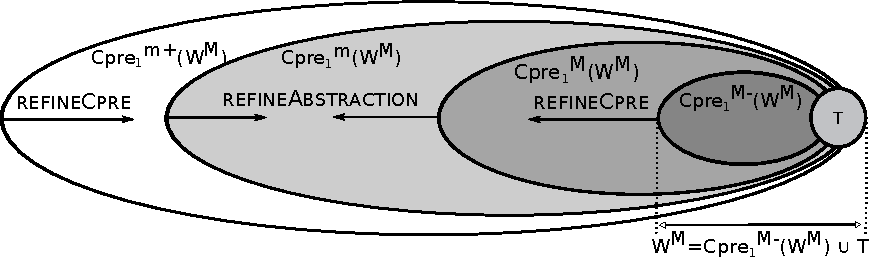
\includegraphics[width=0.85\linewidth]{imgs/approxThreeValue.pdf}
\caption{Overview of approximate three valued abstraction-refinement}
\label{fig:approx_three_val_overview}
\end{figure}


\begin{equation}
\label{eqn:cpre_p1}
\cprem \subseteq \cpremp
\end{equation}

\noindent and

\begin{equation}
\label{eqn:cpre_p2}
\cpreMm \subseteq \cpreM
\end{equation}

With these operators we create a new approximate abstraction-refinement scheme given in Algorithm \ref{alg:approx_three_val}. 

\begin{algorithm}
\caption{Approximate three-valued abstraction-refinement}
\label{alg:approx_three_val}

\begin{algorithmic}[1]

\Require {\bf Input:} A game structure $G = \langle S, L, I, \tau_1, \tau_2, \delta \rangle$, a set 
of target states $T\subseteq S$, and an initial abstraction $\alpha=\langle V, \concrete{}, Cpre_1^{m+}, Cpre_1^{M-} \rangle$
that is precise for $T$, $I$, and $\tau_i$.

\Ensure {\bf Output:} {\it Yes} if $I \subseteq \reach(T, Cpre_1)$, and {\it No} otherwise.

\Function{Solve}{$transitionRelation$, $goal$}
    \Loop
        \State $W^M \gets \reach(\abstractM{T}, Cpre_1^{M-})$
        \State $W^m \gets \reach(\abstractm{T}, Cpre_1^{m+})$
        \If{$\abstractM{I} \subseteq W^M$} \Return Yes \label{alg:atv:t1}
        \ElsIf{$\abstractM{I} \nsubseteq W^m$} \Return No \label{alg:atv:t2}
        \Else       
            \State $refined \gets \Call{refineCpre}{W^M}$
            \State \algorithmicif{} {$(\neg refined)$}
                $\Call{refineAbstraction}{W^M}$
            \algorithmicend \algorithmicif
        \EndIf
    \EndLoop
\EndFunction

\end{algorithmic}
\end{algorithm}

\subsection{Correctness}

If the algorithm terminates then it returns the correct answer. By equations \ref{eqn:cpre_p1} and \ref{eqn:cpre_p2}, 

\begin{equation}
    \reach(\abstractM{T}, \cpreMm) \subseteq \reach(\abstractM{T}, \cpreM)
\end{equation}

\noindent and 

\begin{equation}
    \reach(\abstractm{T}, \cprem) \subseteq \reach(\abstractm{T}, \cpremp)
\end{equation}

\noindent thus, by Equation \ref{eqn:cpre_inclusion}:

\begin{multline}
    \concrete{W^M} = \concrete{\reach(\abstractM{T}, \cpreMm)} \subseteq \\ \reach(T, \cpre) \subseteq \concrete{\reach(\abstractm{T}, \cpremp)} = \concrete{W^m}
\end{multline}

Thus, if we terminate on lines \ref{alg:atv:t1} or \ref{alg:atv:t2} then we terminate with the right answer.

\subsection{Termination}

\todo{Do I just handwave? I need some properties of refineCpre and refineAbstraction}

\section{Abstraction-Refinement for Predicate Abstraction}

The goal of the following sections is to create a symbolic version of algorithm \ref{alg:approx_three_val} adapted to predicate abstraction.

\subsection{Initial Abstraction}

We obtain the initial abstraction by extracting atomic predicates from expressions $T$, $I$, and $\tau_i$, which guarantees that the abstraction is precise for $T$, $I$, and $\tau_i$. While this property is not essential for our approach, we will rely on it to simplify the presentation of the algorithm.

%\subsection{Initial abstraction}
%
%Algorithm~\ref{alg:generic} takes initial abstraction $\alpha$ as 
%one of its inputs. This requires fixing sets of predicates 
%$\Sigma$, $\Omega$, and $\Lambda$, and consistency relations 
%$C^{m+}$ and $C^{M-}$.  We obtain initial state predicates 
%$\Sigma$ by extracting atomic predicates from expressions $T$, 
%$I$, and $\tau_i$, which guarantees that the initial abstraction 
%is precise for $T$, $I$, and $\tau_i$, as required by the 
%algorithm.  Next, we apply the \textsc{Delta} function 
%(Algorithm~\ref{alg:delta}) to predicates in $\Sigma$ to compute 
%initial untracked and label predicates, and the abstract 
%transition relation $\Delta$.  Finally, we assign $C^{m+}=\top$ 
%and $C^{M-}=\bot$.

\subsection{Abstract Transition Relations}
\label{s:cpre}

Following the three-valued algorithm presented in Section~\ref{sec:three_val_abs_ref}, we would like to find an efficient way to compute over- and under-approximations $Cpre^{m+}$ and $Cpre^{M-}$ of the abstract controllable predecessor operators. Recall that computing $Cpre^m$ and $Cpre^M$ precisely is expensive, as it requires applying the controllable predecessor operator to the concrete transition relation $\delta$. We approximate this costly computation by computing the controllable predecessor over the \emph{abstract transition relation} instead. The abstract transition relation of the game is defined over boolean predicate variables and therefore can be manipulated much more efficiently than the concrete one.

We construct the abstract transition relation via efficient syntactic analysis of the concrete transition relation $\delta$. We present the construction assuming that $\delta$ is given in the variable update form, as in Figure~\ref{fig:ex_game_specification}b. A similar construction is possible for specifications written in real-world hardware and software description languages.

For each state predicate in $\Sigma$, we compute the update function by replacing concrete variables in the predicate with their corresponding update functions. We then transform the resulting formula into a boolean combination of atomic predicates over concrete state and label variables.

\begin{ex}
    Let us compute the update function for abstract variable $\sigma_1$ (Figure~\ref{f:ex}d).  Using update functions for $req$ and $dat$ variables (Figure~\ref{f:ex}c), we obtain: 
    
    \begin{multline}
    \sigma_1' = (req' = dat') = \neg(bsy = false) \land (req=dat) \\ \lor (bsy=false) \land (val=req)
    \end{multline}
    
    \noindent This equation contains three atomic predicates: in addition to the existing predicate $\sigma_1 \leftrightarrow (req=dat)$, it introduces new predicates $(bsy=false)$ and $(val=req)$.  

    The first two predicates correspond to existing state variables $\sigma_1$ and $\sigma_2$.  The last predicate is new; hence it is added to set $\Omega$ and a new untracked variable $\omega_1$ is created for it.  By substituting predicates in the equation with corresponding abstract variables, we obtain the following abstract transition relation for $\sigma_1$ in line~11 of the algorithm:
    $\sigma_1' = (\overline{\sigma_2} \land \omega_1) \lor (\sigma_2 \land \sigma1)$
    \qed
\end{ex}

In the general case, the syntactically computed update function for a predicate may depend on existing state predicates in $\Sigma$ as well as new predicates that are not yet part of the abstraction.  The new predicates are partitioned into \emph{untracked predicates} defined over concrete state variables (e.g., $\mathtt{bsy=false}$ in the above example) and \emph{label predicates} that involve at least one concrete label variable (e.g., $\mathtt{val=req}$).  The term ``untracked predicate'' indicates that these predicates are not part of the abstract state space of the game.  Untracked predicates can be seen as partitioning abstract states in $V$ into smaller \emph{untracked sub-states}, as illustrated in Figure~\ref{f:predicates}.

By substituting untracked and label predicates with fresh boolean variables, $\vect{\omega}$ and $\vect{\lambda}$ respectively, we obtain the abstract transition relation $\Delta$ in the form:

$$
\vect{\sigma}'=\Delta(\vect{\sigma},\vect{\omega},\vect{\lambda})
$$

This syntactically computed transition relation contains two sources of imprecision.  

\begin{itemize}
    \item First, untracked variables $\vect{\omega}$ are not part of the abstract state space $\Sigma$ and are therefore treated as external inputs.  
    \item Second, not all abstract labels  are available in all abstract states and hence not all transitions in $\Delta$ correspond to a feasible concrete transition.  For example, given the set of predicates shown in Figure~\ref{f:ex}d, the abstract label $\lambda_1 = true, \lambda_2 = true$ is only available in concrete states that satisfy the condition $req=5$.  In general, given a state-untracked-label tuple $\langle v,u,l\rangle$, the abstract label $l$ may be available in all, some, or none of the concrete states consistent with $v$ and $u$.  
\end{itemize}

\subsection{Consistency Relations}

We formalise this by introducing \emph{consistency relations} $C^m$ and $C^M$ that over- and under-approximate available abstract labels.  A state-untracked-label tuple $\langle v,u,l\rangle$ is \emph{may-consistent} if the abstract label $l$ is available in \emph{at least one} concrete state consistent with $v$ and $u$:

\begin{equation} 
    \label{eqn:cm}
    C^m(v,u,l) = \exists X,Y. \|\vect{\sigma}\|=v \land \|\vect{\omega}\|=u \land \|\vect{\lambda}\|=l.
\end{equation}

The tuple $\langle v,u,l\rangle$ is \emph{must-consistent} if $l$ is available in \emph{any} concrete state consistent with $v$ and $u$:

\begin{equation}
    \label{eqn:cM}
    C^M(v,u,l) = \forall X . ((\|\vect{\sigma}\|=v \land \|\vect{\omega}\|=u) \rightarrow \exists Y.  \|\vect{\lambda}\|=l)
\end{equation}

Computing $C^m$ and $C^M$ can be prohibitively expensive.  Therefore we use approximations $C^{m+}$ and $C^{M-}$ such that 

\begin{equation}
    C^m\subseteq C^{m+}
\end{equation}
and 
\begin{equation}
    C^{M-}\subseteq C^M
\end{equation} 

Initially we assign $C^{m+}=\top$ and $C^{M-}=\bot$.  Approximations are refined lazily as part of the abstraction refinement process, as explained below.

\begin{ex}
    \everymath{\mathtt{\xdef\tmp{\fam\the\fam\relax}\aftergroup\tmp}}
    \everydisplay{\mathtt{\xdef\tmp{\fam\the\fam\relax}\aftergroup\tmp}}
    To illustrate the above definitions, we introduce two label predicates to our running example: $\|\lambda_1\|= (val=req)$, $\|\lambda_2\| = (val=5)$. Consider the state-untracked-label tuple $v=(true,false)$, $u=(true)$, $l=(true, true)$, which corresponds to the following assignment to abstract variables: $\sigma_1=true \land \sigma_2=false \land \omega_1=true \land \lambda_1=true \land\lambda_2=true$. It is easy to see that this condition is satisfied for example by the following concrete variable valuation: $mem=5$, $dat=5$, $bsy=true$, $req=5$, $val=5$, hence $\langle v,u,l\rangle$ is may-consistent: $C^m(v,u,l)=true$.  However, it is not must-consistent:

    $$
    \begin{aligned}
        C^M(v,u,l) = \forall  mem, dat, bsy,req. (&((req=mem) \land (bsy = true) \land (req=dat)) \rightarrow \\
                                                  &\exists val. (val=req) \land (val=5))
    \end{aligned}
    $$
    
    There exist concrete state variable assignments (e.g., $mem=1$, $dat=1$, $bsy=true$, $req=1$) that satisfy state and untracked predicates in the left-hand side of the implication but that can not be extended with a label variable assignment that satisfies the right-hand side, hence $C^M(v,u,l)=false$.  
    \qed
\end{ex}

\subsection{Abstract Controllable Predecessor}

We compute over- and under-approximations of the controllable predecessor operator by resolving the two sources of imprecision in favour of one of the players.  In particular, we compute $Cpre_i^{m+}$ by (1) allowing player $i$ to pick assignments to untracked predicates, (2) over-approximating consistent labels available to $i$, and (3) under-approximating consistent labels available to the opponent player $\overline{i}$:

\begin{equation}
    \label{e:cprem}
    \small
\begin{aligned}
    Cpre_i^{m+}(\phi) = \exists \vect{\omega} .~&\abstractM{\tau_i}         \land \exists \vect{\lambda},\vect{\sigma'}. ((C^{m+} \land \Delta) \land \phi')
                                                 ~~\lor\\
                                                &\abstractM{\tau_{\overline{i}}} \land \forall \vect{\lambda},\vect{\sigma'}. ((C^{M-} \land\Delta) \rightarrow \phi')
\end{aligned}
\end{equation}

This formula has a similar structure to the definition of the concrete controllable predecessor operator (\ref{e:cpre}).  It replaces the concrete transition relation $\delta$ with the abstract transition relation $\Delta$ restricted with consistency relations ($C^{m+}$ and $C^{M-}$).  In addition, it existentially quantifies untracked variables $\vect{\omega}$, i.e., an abstract state $v$ is a may-predecessor of $\phi$ if at least one of its untracked sub-states is a may-predecessor of $\phi$.

Dually, we compute $Cpre_i^{M-}$ by (1) allowing the opponent player $\overline{i}$ to pick values of untracked predicates, (2) under-approximating labels available to $i$ and (3) over-approximating labels available to $\overline{i}$:

\begin{equation}
    \small
    \label{e:cpreM}
\begin{aligned}
    Cpre_i^{M-}(\phi) = \forall \vect{\omega}.~&\abstractM{\tau_i}         \land \exists \vect{\lambda},\vect{\sigma'}. ((C^{M-} \land \Delta) \land \phi')
                                             ~~\lor\\
                                               &\abstractM{\tau_{\overline{i}}} \land \forall \vect{\lambda},\vect{\sigma'}. ((C^{m+} \land \Delta) \rightarrow \phi')
\end{aligned}
\end{equation}

Note that the use of $C^{m+}$ and $C^{M-}$ in (\ref{e:cprem}) and (\ref{e:cpreM}) under-constrains moves available to player~$i$ and over-constrains moves available to the opponent.  The formula for $CpreU_i^{M-}(\phi)$ is analogous, except that it over-constrains moves available to $i$ and under-constrains moves available to $\overline{i}$.

Equations (\ref{e:cprem}) and (\ref{e:cpreM}) suggest two possible abstraction refinement tactics, which correspond to the two types of refinement used in Algorithm~\ref{alg:generic}.  First, we can refine $C^{m+}$ and $C^{M-}$ by removing spurious transitions from $C^{m+}$ or adding new consistent transitions to $C^{M-}$.  Such a refinement increases the precision of controllable predecessor computation without introducing new state predicates, which corresponds to the \textsc{refineCpre} operation in the algorithm.  Second, we can add some of the untracked predicates to the set of state predicates $\Sigma$, thus reducing the imprecision introduced by treating them as external inputs.  This refinement increases the precision of the abstraction, which corresponds to the \textsc{refineAbstraction} function in the algorithm.

In summary, we solve the abstract game by decomposing potentially expensive computations into four types of light-weight operations performed on demand, as required to improve the precision of the abstraction:

\begin{itemize}
    \item Computing the abstract transition relation $\Delta$ via light-weight syntactic analysis of the concrete game
    \item Computing consistency relations $C^{m+}$ and $C^{M-}$ by iteratively identifying spurious and consistent transitions
    \item Iteratively refining the abstraction used in the syntactic computation of the transition relation
    \item Solving the abstract game using abstract controllable predecessor operators (\ref{e:cprem}) and (\ref{e:cpreM})
\end{itemize}

The computational bottleneck in this method can arise either from having to perform an excessive number of refinements or if abstractions generated by the algorithm are too complex.  Our refinement procedures, described below, are designed to avoid such situations by heuristically picking refinements that are likely to speed up the convergence of the algorithm.

%\subsection{Abstract transition relation}
%
%The \emph{abstract transition relation}
%$\Delta: \mathbb{B}^n \times \mathbb{B}^k \times \mathbb{B}^m 
%\rightarrow 2^{\mathbb{B}^n}$
%of the game maps an assignment of state, untracked, and label 
%predicates to the set of possible next states.  The arrow in 
%Figure~\ref{f:predicates} illustrates a transition from untracked 
%sub-state $u$ of state $v$ to state $v'$ via abstract label $l$.  
%Note that the source of an abstract transition is a pair of state 
%and untracked predicate assignments, while the target of the 
%transition is an assignment to state predicates only.
%
%Algorithm~\ref{alg:delta} shows the pseudocode of function 
%\textsc{Delta}.  It takes a list of state predicates and returns 
%the abstract transition relation $\Delta$ along with untracked and 
%label predicates used in $\Delta$.
%It assumes that the concrete transition relation $\delta$ of the 
%game is specified in the form of variable update functions $x' = 
%t_x(X,Y)$, as in Figure~\ref{f:ex}b.
%
%\begin{algorithm}[t]
%\caption{Pseudocode for computing the abstract transition relation.}
%\label{alg:delta}
%\begin{algorithmic}[1]
%    \Function{Delta}{$\vect{\sigma}=(\sigma_1\ldots\sigma_n)$ - state predicate variables}
%        \For{$i = 1 \text{ to } n$}
%            \State $t_{\sigma_i} \gets \|\sigma_i \|[x \mid t_x(X,Y), \text{for all } x\in X]$
%            \State $t_{\sigma_i} \gets $ \Call{massage}{$t_{\sigma_i}$}
%        \EndFor
%        \State $P \gets \bigcup_i \text{atomic predicates in }t_{\sigma_i}$
%        \State $\Omega \gets \text{state predicates in } P \setminus \Sigma$
%        \State $\Lambda \gets \text{label predicates in } P \setminus \Sigma$
%        \State $\vect{\omega}\gets \text{fresh variables for predicates in } \Omega$
%        \State $\vect{\lambda} \gets \text{fresh variables for predicates in } \Lambda$
%        \State $\Delta \gets \bigwedge_i (\sigma_i' = t_{\sigma_i}[\|\alpha\|\mid \alpha, \text{for all } \alpha\in\vect{\sigma}\cup\vect{\omega}\cup\vect{\lambda}])$
%        \State \Return $\langle \vect{\omega}, \vect{\lambda}, \Delta \rangle$
%    \EndFunction
%\end{algorithmic}
%\end{algorithm}
%
%Lines 2--5 of the algorithm compute update functions for predicate 
%variables $\sigma_i$ by replacing each variable $x$ in predicate 
%$\|\sigma_i\|$ by its update function $t_x$.  The \textsc{massage} 
%function transforms the resulting expression $t_{\sigma_i}$ into a 
%boolean combination of atomic predicates over $X \cup Y$.  In 
%line~6 we collect all predicates found in $t_{\sigma_i}$.  The 
%resulting set $P$ may contain predicates not found in $\Sigma$.  
%Such predicates are classified into untracked predicates $\Omega$ 
%defined over state variables only and label predicates $\Lambda$ 
%that involve at least one label variable from $Y$ (lines~7--8).  
%The abstract transition relation $\Delta$ is computed by replacing 
%all boolean predicates in $t_{\sigma_i}$ with corresponding 
%boolean variables (line~11).
%
%\begin{ex}
%    \everymath{\mathtt{\xdef\tmp{\fam\the\fam\relax}\aftergroup\tmp}}
%    \everydisplay{\mathtt{\xdef\tmp{\fam\the\fam\relax}\aftergroup\tmp}}
%    Let us compute the update function for abstract variable 
%    $\sigma_1$. Recall that $\|\sigma_1\| = (req=mem)$.  Using 
%    update functions for $req$ and $mem$ variables from 
%    Figure~\ref{f:ex}b, we obtain:
%    $t_{\sigma_1} = (t_{req}(X,Y)=t_{mem}(X,Y)) = \bigg(req = 
%    \begin{cases}
%        dat, & \text{if } \neg bsy\\
%        mem, & \text{otherwise}
%    \end{cases}\bigg).$  The \textsc{massage} function transforms 
%    this into:
%    $t_{\sigma_1} = \big((bsy = true \land req=dat) \lor 
%    (bsy=false \land req=mem)\big)$.
%    This equation contains three predicates: $(req=mem)$, 
%    $(bsy=false)$ (and its negation), and $(req=dat)$.  The first 
%    two predicates correspond to existing state variables 
%    $\sigma_1$ and $\sigma_2$.  The last predicate is new; hence 
%    it is added to set $\Omega$ and a new untracked variable 
%    $\omega_1$ is created for it.  By substituting predicates in 
%    the equation with corresponding abstract variables, we obtain 
%    the following abstract transition relation for $\sigma_1$ in 
%    line~11 of the
%    algorithm:
%    $\sigma_1' = (\overline{\sigma_2} \land \omega_1) \lor (\sigma_2 \land \sigma1)$
%    \qed
%\end{ex}
%
%The above algorithm has the useful property that $\Delta$ is 
%computed via simple syntactic transformations of the concrete 
%game specification. Additionally, untracked predicates discovered 
%by the algorithm are known to influence the values of state 
%predicates in $\Sigma$. As such, these predicates constitute 
%potentially useful candidates for promotion to state predicates 
%as part of the abstraction refinement process.

\subsection{Consistency Refinement}

Figure~\ref{f:crefinement} illustrates the main idea of the consistency refinement algorithm.  It shows an abstract state $v$ (Figure~\ref{f:crefinement}a) at the may-must boundary whose untracked substates $u_1$, $u_2$, and $u_3$ have $C^{m+}$-consistent transitions to the must-winning set $W^M$, but none of these transitions is consistent with $C^{M-}$.  The \textsc{refineCpre} algorithm attempts to precisely categorise these substates as must-winning or must-losing.

Since all untracked substates of $v$ are either must-losing or may-winning but not must-winning, it is impossible to split out a must-winning subset of $v$ purely by predicate promotion; hence a consistency refinement is needed.

The consistency refinement algorithm proceeds in one of three ways:
\begin{itemize}
    \item In Figure~\ref{f:crefinement}b, the algorithm identifies the abstract transition $\langle v,u_1, l_1\rangle$ as spurious and eliminates it from $C^{m+}$, thus making the $u_1$ sub-state must-losing.  
    \item Alternatively, it may detect that abstract transition $\langle v, u_2, l_2\rangle$ is available in all concrete states in $u_2$ and thus add this transition to $C^{M-}$, making the $u_2$ sub-state must-winning (Figure~\ref{f:crefinement}c).  
    \item Finally, it may determine that abstract transition $\langle v, u_3, l_3\rangle$ is available in some, but not all, concrete states in $u_3$, i.e., $\langle v, u_3, l_3\rangle\in C^m\setminus C^M$.  It then partitions $u_3$ into two or more subsets, exactly one of which has a $C^{M-}$-consistent transition to $W^M$, by introducing new untracked predicates (Figure~\ref{f:crefinement}d).  
\end{itemize}

In all three cases, further refinement via untracked predicate promotion becomes possible.  Such refinement is performed by the \textsc{refineAbstraction} function described in Section~\ref{s:refineAbstraction}.

\begin{figure}[t]
    \label{f:crefinement}
    \center
    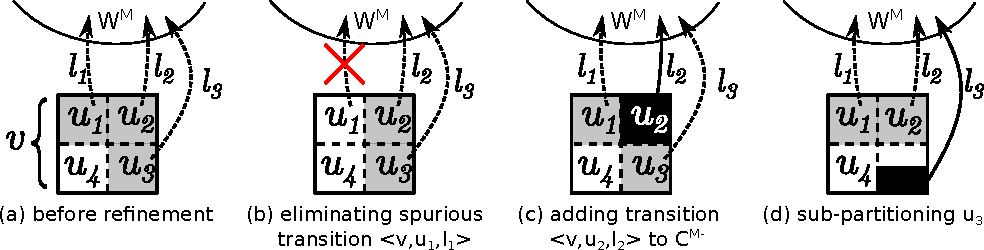
\includegraphics[width=\linewidth]{imgs/crefinement}
    \caption{Different types of consistency refinements.  White, grey, and black background is used to mark respectively must-losing, may-winning, and must-winning untracked substates.  Dashed and solid arrows show $C^{m+}$ and $C^{M-}$-consistent abstract transitions.}
\end{figure}

Note that in the special case when, after performing consistency refinement, all untracked substates of $v$ become must-winning or must-losing, the entire state $v$ can be removed from the boundary region without performing predicate promotion.  This corresponds to the two types of refinement labelled as \textsc{refineCpre} in Figure~\ref{f:reach}.  

For this reason, Algorithm~\ref{alg:generic} recomputes $W^M$ and $W^m$ after each successful consistency refinement, and only calls \textsc{refineAbstraction} once no more consistency refinements are possible.

\subsection{Algorithm}

Algorithm~\ref{alg:refineCpre} shows the pseudocode of \textsc{refineCpre}.  Lines~3--6 compute the set of candidate tuples $\langle v, u, l\rangle\in C^m\setminus C^M$.  Note that for player~$i$ states we consider may-consistent transition to $W^M$, whereas for player~$\overline{i}$ states we consider spoiling transitions to $V\setminus W^M$.

Line~9 picks a single refinement candidate $\langle v,u,l \rangle$ from the set.  By construction we know that $\langle v,u,l\rangle\in C^{m+}$.  Since $C^{m+}$ is an overapproximation of $C^m$, we check whether $\langle v,u,l\rangle\in C^m$, i.e., whether $v$, $u$, and $l$ satisfy equation (\ref{e:Cm}).  To this end, in line~11 we invoke a decision procedure for the underlying theory to check satisfiability of the formula:$(\|\vect{\sigma}\|=v \land \|\vect{\omega}\|=u \land \|\vect{\lambda}\|=l)$.If the formula is unsatisfiable, then $\langle v,u,l\rangle$ is a spurious transition that must be eliminated from $C^{m+}$.  Furthermore, by extracting an unsatisfiable core of the formula,we obtain an inconsistent subset of its conjuncts $(\bigwedge\|\alpha_i\|=c_i)$, $\alpha_i\in\vect{\sigma}\cup\vect{\omega}\cup\vect{\lambda}$,which represents a potentially large set of similar spurioustransitions.  We eliminate all of these transitions from $C^{m+}$ inline~16.

\begin{algorithm}[t]

\caption{Pseudocode of the \textsc{refineCpre} function}
\label{alg:refineCpre}
\begin{algorithmic}[1]
\Function{refineCpre}{$W^M$}
    \State \Comment{player~$i$ may-winning transitions}
    \State $T_i         \gets \abstractM{\tau_i} \land C^{m+} 
    \land {\overline{C^{M-}}} \land \forall \vect{\sigma'}. (\Delta \rightarrow (W^M)')$
    \State \Comment{player~$\overline{i}$ may-spoiling transitions}
    \State $T_{\overline{i}} \gets \abstractM{\tau_{\overline{i}}} \land C^{m+} \land {\overline{C^{M-}}} \land \exists \vect{\sigma'}. (\Delta \land \overline{(W^M)'})$
    \State $T           \gets T_i \lor T_{\overline{i}}$
    \If{$T = \bot$}
        \Return $false$ \Comment{no refinement is possible}
    \Else
        \State choose $\langle v,u,l\rangle \in T$
        \State $F \gets (\|\vect{\sigma}\|=v \land \|\vect{\omega}\|=u \land \|\vect{\lambda}\|=l)$
        \If{\Call{satisfiable}{$F$}}
            \State $A             \gets $ \Call{eliminateQuantifiers}{$\exists Y.\|\vect{\lambda}\|=l$}
            \State $A             \gets $ \Call{massage}{$A$}
            \State $P             \gets \text{atomic predicates in }A$
            \State $\vect{\omega} \gets \vect{\omega} \cup (\text{fresh variables for predicates in } P\setminus\Omega)$
            \State $\Omega        \gets \Omega \cup P$
            \State $\hat{A}       \gets A[\|x\|\mid x, \text{for all } x\in\Omega \cup \Sigma ]$
            \State $\hat{A}       \gets$ replace atomic predicates in $A$ with boolean
            \Statex  ~~~~~~~~~~~~~~~~~~~~vars, introducing fresh vars when necessary
            \State $C^{M-}        \gets C^{M-} \lor (\hat{A}\land \vect{\lambda}=l)$% \Comment{add consistent transition}
        \Else
%            \State $(\bigwedge\|\alpha_i\|=c_i) \gets$ \Call{unsatCore}{$F$}
            \State $C^{m+}\gets C^{m+} \land \overline{\textsc{unsatCore}(F)}$ %\Comment{eliminate spurious transitions}
        \EndIf
        \State \Return $true$
    \EndIf
\EndFunction
\end{algorithmic}
\end{algorithm}

If, on the other hand, the formula is satisfiable, then there exists a concrete state-label pair consistent with $\langle v,u,l\rangle$.  In this case we want to precisely characterise the set of states where label $l$ is available, so that we can either add $\langle v,u,l\rangle$ to $C^{M-}$ (as in Figure~\ref{f:crefinement}c) or refine it with additional untracked predicates (as in Figure~\ref{f:crefinement}d).

Line~12 computes the set of concrete states where abstract label $l$ is available by performing quantifier elimination from formula $(\exists Y.\|\vect{\lambda}\|=l)$, resulting in a quantifier-free formula $A$ over concrete state variables $X$.  We assume that the underlying theory supports quantifier elimination, which is the case for many practically relevant theories, including the theory of fixed-size bit vectors supported by our tool.  In line~13, the resulting formula $A$ is decomposed into atomic predicates possibly introducing new untracked and label predicates.  By replacing all atomic predicates in $A$ with corresponding boolean variables, we obtain a formula $\hat{A}$ that describes the set of all state-untracked pairs must-consistent with the abstract label $l$.  Line~14 refines $C^{M-}$ with the set of newly discovered must-consistent transitions.

%The resulting formula is decomposed into atomic predicates 
%(lines~11--12).  New predicates from $A$ are added to the set of 
%untracked predicates (lines~13--14).  Finally, all predicates in 
%$A$ are replaced with corresponding boolean variables (line~15) 
%and the resulting formula over abstract variables is used to 
%refine the must consistency relation $C^{M-}$ (line~16).  

\begin{ex}
    \everymath{\mathtt{\xdef\tmp{\fam\the\fam\relax}\aftergroup\tmp}}
    \everydisplay{\mathtt{\xdef\tmp{\fam\the\fam\relax}\aftergroup\tmp}}
    Assume that in line~9 the algorithm picks a tuple $\langle 
    v,u,l\rangle$ where $l=(true, true)$.  Line~12 performs 
    quantifier elimination from the formula $\exists val.  
    (\|\lambda_1\|=true \land  \|\lambda_2\|=true) =
    \exists val. (val=req \land val=5) = (req=5)$.
%    , i.e., conditions $(val=req)$ and $(val=5)$ can only hold 
%    simultaneously if $(req=5)$.
    We have discovered a new predicate $req=5$ that 
    must hold in states where abstract label $l$ is 
    available.  We introduce a new untracked variable $\omega_2$, 
    $\|\omega_2\|=(req=5)$ and refine $C^{M-}$ with a new 
    consistent transition: $C^{M-} \gets C^{M-} \lor (\omega_2 
    \land \lambda_1 \land \lambda_2)$.
    \qed
\end{ex}

\subsection{Refining the Abstraction}
\label{s:refineAbstraction}

The \textsc{refineAbstraction} function is invoked by the abstraction refinement algorithm when no further consistency refinements are possible.  At this point, every untracked sub-state of the boundary region is either must-winning or must-losing, i.e., can be coloured white or black using notation of Figure~\ref{f:crefinement}.  \textsc{refineAbstraction} promotes a subset of untracked predicates making sure that the winning region $W^M$ expands after re-solving the game in line~2 of Algorithm~\ref{alg:generic}.  

Algorithm~\ref{alg:refineAbstraction} shows the pseudocode of \textsc{refineAbstraction}.  Line~2 computes all untracked boundary substates that are must-predecessors of $W^M$.  Here, $CpreU^{M-}$ is the same as $Cpre^{M-}$ (Equation~(\ref{e:cpreM})), but without untracked variable quantification:

$$
    \small
\begin{aligned}
    CpreU_i^{M-}(\phi) = &\abstractM{\tau_i}         \land \exists \vect{\lambda},\vect{\sigma'}. ((C^{M-} \land \Delta) \land \phi')
                          ~~\lor\\
                         &\abstractM{\tau_{\overline{i}}} \land \forall \vect{\lambda},\vect{\sigma'}. ((C^{m+} \land \Delta) \rightarrow \phi')
\end{aligned}
$$

We aim to grow  $W^M$ by promoting as few untracked predicates as possible.  To this end, we extract a short prime implicant from $U^M$ and promote the untracked variables in the support of the prime implicant (line~3).  This has the effect of adding a large cube over state and untracked predicates to $W^M$. The \textsc{promote} function invoked on line~4 moves the selected untracked predicates to the set of state predicates $\Sigma$ and recomputes the abstraction transition relation $\Delta$ for the new state predicates.  This can lead to the introduction of new untracked and label predicates, which can serve as refinement candidates in the future.

\begin{algorithm}[t]

\caption{Pseudocode of \textsc{refineAbstraction}}
\label{alg:refineAbstraction}

\begin{algorithmic}[1]

\Function{refineAbstraction}{$W^M$}
    \State $U^M \gets CpreU_1^{M-}(W^M) \land \overline{W^M}$
    \State $toPromote \gets \vect{\omega}~\cap~$\Call{support}{\textsc{shortPrime}($U^M$)}
    \State $\Call{promote}{toPromote}$
\EndFunction

\end{algorithmic}
\end{algorithm}

We must be careful when refining the abstraction. Do our consistency constraints remain valid after the abstraction has been refined? The following example shows that in some cases they do not.

\begin{ex}
    Consider an abstraction of the running example game induced by abstract variable $\sigma_1$ with corresponding predicate $\|\sigma_1\| = (req=dat)$ as well as the abstract label variable $\lambda_1$ with corresponding predicate $\|\lambda_1\| = (val=req)$. There are no untracked variables.

    Our must consistency constraint, $C^{M-}$, is a relation over the variables $\sigma_1$ and $\lambda_1$. For example, the tuple $v=(true), l=(true)$ is must consistent because it is always possible to assert $\lambda_1=true$ when $\sigma_1=true$ by choosing $val$ appropriately.

    Suppose, when computing the update function for some variable that has just been promoted we introduce the abstract untracked variable $\omega_2$ with corresponding predicate $\|\omega_2\| = (req=5)$. This partitions each sub-state into two. The definition of $C^{M-}$ (Equation \ref{eqn:cM}) ensures that if a label is must consistent in a given state before the variable promotion then it will be must consistent in each sub-state after the promotion. In this example, the tuples $v=(true), u=(false), l=(true)$ and $v=(true), u=(true), l=(true)$ are both must consistent. Notice that, if we are symbolically representing $C^{M-}$, then the new $C^{M-}$ does not depend on the newly introduced untracked variable. Thus, we may keep the same $C^{M-}$ from before the promotion.

    The situation is not so good for promotions that introduce new label variables. We cannot simply reuse $C^{M-}$ from before the variable promotion as we do for untracked variables. Consider what happens when, continuing on from before, we add $\lambda_2$ with corresponding predicate $\|\lambda_2\| = (val=5)$. The tuple $v=(true), u=(true), l=(true)$ is must consistent. Extending the tuple to $v=(true), u=(true), l=(true, true)$ is fine, but $v=(true), u=(true), l=(true, false)$ is not. The latter tuple is not must-consistent. Therefore, we may not simply reuse $C^{M-}$ as in the case where an untracked variable is added. 

    We can rebuild $C^{M-}$ by considering all possible tuples with the additional label. In this case as there are few variables this would work and we would discover that the second tuple above is not part of $C^{M-}$. However, when there are more variables this is infeasible. 

    \qed
\end{ex}

From this example, we make two important observations. When compiling the update function for a untracked predicate that is being promoted to a state predicate when refining the abstraction, 

\begin{itemize}
    \item if the compilation only introduces new untracked predicates, then we can keep the consistency relations from the previous iteration.
    \item if the compilation introduces new label predicates, then we cannot reuse $C^{M-}$ from the previous iteration without modification.
\end{itemize}

We resort to conservatively resetting $C^{M-}$ to $false$ when a new label variable is added and incrementally rebuilding $C^{M-}$ lazily as before. This is a severe performance impediment as $C^{M-}$ may have to be rebuilt many times. We present a pragmatic solution to this problem that is used by Termite in Section \ref{sec:optimisation}.

\subsection{Consistency of the Initial Set}

The last remaining step of the approximate three valued abstraction-refinement algorithm is checking whether the winning set contains the initial set. Again, predicate abstraction complicates things as the following example shows.

\begin{ex}
    Consider an abstraction of the running example induced by the abstract variables $\sigma_1$, $\sigma_2$ and $\sigma_3$ and corresponding predicates $\|\sigma_1\| = (req=dat)$, $\|\sigma_2\| = (req=mem)$ and $\|\sigma_3\| = (dat=mem)$. The initial set is specified as $req=dat \land req=mem$ which is abstracted to $\sigma_1 \land \sigma_2$. Suppose that the may winning set of states, $W^{m+}$, that the game solving algorithm returns is $\{v=(true, true, true)\}$. Importantly, this set does not contain $v=(true, true, false)$. Naively, we might check if the initial set implies the winning set, i.e., if $(\sigma_1 \land \sigma_2) \rightarrow W^{m+}$. However, as $\sigma_1 \land \sigma_2 \land \neg\sigma_3$ is not part of $W^{m+}$, this implication is false i.e. $(\sigma_1 \land \sigma_2) \centernot\rightarrow (\sigma_1 \land \sigma_2 \land \sigma_3)$.

    We should have ignored the losing state $v=(true, true, false)$ when checking if the winning set consumes the initial set as it is inconsistent and does not correspond to any real states in the concrete game. 

    \qed
\end{ex}

As the example shows, checking if the initial set implies each of the winning sets is not correct. We modify the check to find a witness losing state and we then check consistency of this state. If the state is consistent, then we have found at least one losing concrete state. Otherwise, we extract an unsatisfiable core and add this to a consistency constraint that prevents this and other states from being selected as witnesses in the future. Effectively, we have another refinement loop that iteratively refines a consistency relation over states. The algorithm is given in Algorithm \ref{alg:initial_inclusion}.

\begin{algorithm}
\caption{Checking inclusion of the initial set}
\label{alg:initial_inclusion}

\begin{algorithmic}[1]

\Function{refineInit}{$W$, $Init$, $inconsistent$}
    \If{$Init \rightarrow W$}
        \State\Return $True$
    \Else
        \State $witnesses \gets Init \land \neg W \land \neg inconsistent$
        \State $implicant \gets \Call{primeImplicant}{witnesses}$
        \If{$\Call{satisfiable}{implicant}$}
            \State\Return $False$
        \Else
            \State $inconsistent \gets inconsistent \lor \Call{unsatCore}{implicant}$
            \State\Call{refineInit}{$W$, $Init$, $inconsistent$}
        \EndIf
    \EndIf
\EndFunction

\end{algorithmic}
\end{algorithm}

\subsection{Putting it Together}

\begin{algorithm}
\caption{Three-valued abstraction refinement for games.}
\label{alg:genericc}

\begin{algorithmic}[1]

\Function{Solve}{$transitionRelation$, $goal$}
    \Statex {\bf Input:} A game structure $G = \langle S, L, I, \tau_1, \tau_2, \delta \rangle$, a set 
    of target states $T\subseteq S$, and an initial abstraction $\alpha=\langle V, \concrete{}, Cpre_1^{m+}, Cpre_1^{M-} \rangle$
    that is precise for $T$, $I$, and $\tau_i$.

    \Statex {\bf Output:} {\it Yes} if $I \subseteq \reach(T, Cpre_1)$, and {\it No} otherwise.

    \Loop
        \State $W^M \gets \reach(\abstractM{T}, Cpre_1^{M-})$
        \State $W^m \gets \reach(\abstractm{T}, Cpre_1^{m+})$
        \If{$\abstractM{I} \subseteq W^M$} 
            \State\Return Yes
        \ElsIf{$\abstractM{I} \nsubseteq W^m$} 
            \State\Return No
        \Else       
            \State $refined \gets \Call{refineCpre}{W^M}$
            \If {$(\neg refined)$}
                \State$\Call{refineAbstraction}{W^M}$
            \EndIf
        \EndIf
    \EndLoop
\EndFunction

\end{algorithmic}
\end{algorithm}


\subsection{Correctness}

The correctness and termination theorems of~\cite{Alfaro_Roy_07} hold for Algorithm~\ref{alg:generic} with \textsc{refineCpre} and \textsc{refineAbstraction} functions defined above.

\begin{theorem}

If Algorithm~\ref{alg:generic} terminates, it returns the correct answer.

\end{theorem}

\begin{proof}

By construction, $Cpre_i^{m+}$ and $Cpre_i^{M-}$ over- and under-approximate abstract controllable predecessor operators, i.e., $\concrete{Cpre_i^m(\phi)} \subseteq \concrete{Cpre_i^{m+}(\phi)}$ and $\concrete{Cpre_i^{M-}(\phi)} \subseteq \concrete{Cpre_i^M(\phi)}$, for any set $\phi$.  Hence, winning sets $W^m = \reach(\abstractm{T}, Cpre_1^{m+})$ and $W^M = \reach(\abstractM{T}, Cpre_1^{M-})$ computed using these operators over- and under-approximate the winning set $W$ of the concrete game: $\concrete{W^M}\subseteq W \subseteq \concrete{W^m}$.  

If the algorithm returns \emph{Yes} then the initial set of the game is a subset of the must-winning region ($I\subseteq \concrete{W^M}$) and hence $I\subseteq W$.  Likewise, if the algorithm returns \emph{No} then $I\not\subseteq \concrete{W^m}$ and hence $I\not\subseteq W$.  In both cases the answer produced by the algorithm is correct.

\end{proof}

\begin{theorem}
\label{t:termination}

If there exists a finite region algebra $\mathcal{A}$ such that all abstractions $\langle V, \concrete{}\rangle$ produced by Algorithm~\ref{alg:generic} are contained in $\mathcal{A}$ then the algorithm terminates.

\end{theorem}

\begin{proof}[Proof outline]

Let $W^M$ and $\hat{W}^M$ be must-winning sets computed at two subsequent iterations of Algorithm~\ref{alg:generic}.  

We first show that refinement procedures \textsc{refineCpre} and \textsc{refineAbstraction} guarantee that the must-winning set computed at every iteration of the refinement loop grows monotonically, i.e., $\concrete{W^M} \subseteq \concrete{\hat{W}^M}$.  This follows from the soundness of the refinement procedures, which improve the precision of $Cpre_i^{M-}$ at every iteration. 

Next we show that the algorithm is guaranteed to make forward progress, i.e., after a finite number of refinements it either terminates or discovers new must-winning states ($\concrete{W^M} \subset \concrete{\hat{W}^M}$).  Consider the consistency refinement procedure \textsc{refineCpre} first.  Every invocation of this procedure classifies some of the untracked substates at the may/must boundary as either must-winning or must-losing (see Figure~\ref{f:crefinement}).  Eventually, it will either classify all boundary states as must-losing, in which case $\concrete{W^m} = W = \concrete{W^M}$, and the algorithm terminates, or find at least one must-winning sub-state (as in Figures~\ref{f:crefinement}c and~\ref{f:crefinement}d).  In the latter case, a subsequent invocation of the abstraction refinement procedure \textsc{refineAbstraction} is guaranteed to partition one of the boundary states so that one of the resulting abstract states is must-winning.  This state will be discovered at the next run of the reachability algorithm, thus expanding the must-winning set.

Since, by the assumption of the theorem, all must-winning sets $W^M$ generated by the algorithm belong to a finite region algebra, the algorithm is guaranteed to terminate after a finite number of iterations.

\end{proof}

The theory of fixed-size bit vectors supported by our current implementation satisfies the premise of Theorem~\ref{t:termination}, which guarantees the termination of the algorithm.

\section{Optimisation}
\label{sec:optimisation}

Algorithm~\ref{alg:refineCpre} has two important performance issues: 

\begin{itemize}

    \item Every time an untracked variable is promoted, if a new label variable is created in the process, $C^{M-}$ must be reset to False.

    \item In lines~10--16 it analyses and adds to $C^{M-}$ a single abstract label $l$.  The set of all abstract labels is exponential in size in the number of label predicates and can be very large in practice, making explicit enumeration infeasible.  

\end{itemize}

To address the first issue, we modify the algorithm to handle a set of abstract labels at every iteration.  To this end, in line~7, instead of choosing a complete assignment to state, untracked, and label predicates, we compute a \emph{prime implicant} of set $T$, i.e., an assignment to a subset of variables in $\vect{\sigma}\cup\vect{\omega}\cup\vect{\lambda}$ such that any extension of this assignment to the remaining variables satisfies $T$: 
$$
\langle v,u,l\rangle \gets \textsc{primeImplicant}(T),
$$ 
where $v$, $u$, and $l$ are partial valuations of abstract variables, which compactly represent a potentially large set of abstract transitions.  In practice, we typically discover prime implicants that only constrain few of the abstract variables, meaning that other predicates are irrelevant for the outcome of the transition.  

Given this modification, the $C^{m+}$ refinement case of the algorithm (lines~18--19) is still correct and does not require any changes.  However, changes are needed in the $C^{M-}$ refinement logic.  The set $A$ computed in lines~10--1 contains all concrete states where \emph{at least one} abstract label from the set characterised by the partial assignment $l$ of label predicates is available.  It does not guarantee the availability of any particular label from this set.  To model this constraint, we would have to change $C^{M-}$ to be a relation over sets of labels.  Every element of the relation would describe a set of labels, one of which is guaranteed to be available for the given state and untracked predicate assignment.  

This introduces a new form of imprecision to the consistency relation: rather than categorising each abstract label as available or unavailable in the given state, we record a set of labels, one of which is available.  However, such a relation would be hard to represent and manipulate efficiently in the symbolic form.  Therefore, we propose a different approach that allows symbolic implementation.  

We transform the game (without changing its winning set) in order to solve it more efficiently.  The idea of our solution is to model the new form of imprecision as non-determinism in the abstract transition relation $\Delta$.  For each abstract label variable $\lambda_i$, we introduce an auxiliary \emph{enabling variable} $\varepsilon_i$ and transform the transition relation $\Delta$ as follows:
$$
\Delta \gets (\varepsilon_i \land \Delta) \lor (\overline{\varepsilon_i} \land \exists \lambda_i. \Delta).
$$
When $\varepsilon_i=true$, $\Delta$ behaves exactly as before.  In case $\varepsilon_i=false$, the value of $\lambda_i$ chosen by the player is ignored and the environment non-deterministically selects next-state variables assignment that is consistent with \emph{some} assignment of $\lambda_i$. 

We can now modify line~16 of Algorithm~\ref{alg:refineCpre} as follows:
$$
C^{M-} \gets C^{M-} \lor (\hat{A}\land \bigwedge_{i\in{j_1\ldots j_p}}\lambda_i=l_i \land \bigwedge_{i\not\in{j_1\ldots j_p}}\varepsilon_i=false),
$$
where $j_1\ldots j_p$ are indices of variables assigned by $l$.  The above statement refines $C^{M-}$ by allowing the player to assign a subset of label variables in accordance with $l$ and disabling other label variables not constrained by $l$.  The environment will non-deterministically pick arbitrary values for these variables.  In this way we precisely capture what we currently know about consistent predicate assignments in a symbolic form, at the cost of introducing extra variables $\varepsilon_i$.


\chapter{User guided synthesis}
\label{ch:userguided}

\section{Introduction}\label{sec:user_guided_intro}

\subsection{Overview of \termite} Figure~\ref{f:termite} gives an overview of the driver synthesis process, described in detail in the rest of this chapter.  \termite takes three specifications as its inputs: a device model that simulates software-visible device behavior, an OS model that specifies the software interface between the driver and the OS, and a driver template that contains driver entry point declarations and, optionally, their partial implementation to be completed by \termite.

\begin{figure}
    \center
    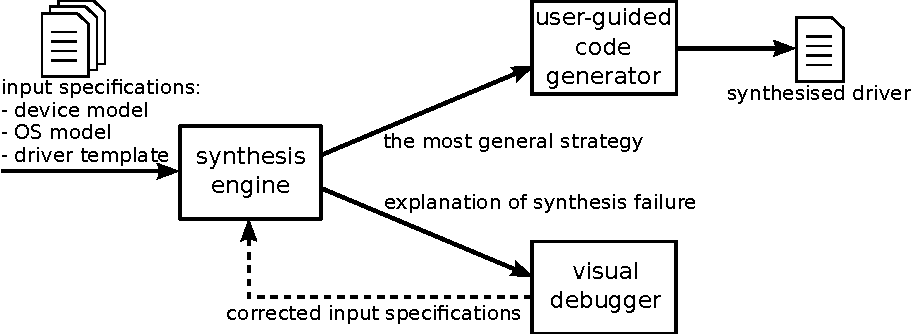
\includegraphics[width=\linewidth]{imgs/termite.pdf}
    \caption{\termite synthesis workflow.}\label{f:termite}
\end{figure}

Given these specifications, driver synthesis proceeds in two steps.  The first step is carried out fully automatically by the \termite game-based synthesis engine, which computes \emph{the most general strategy} for the driver---a data structure that compactly represents all possible correct driver implementations.  This step encapsulates the computationally expensive part of synthesis.  At the second step, the most general strategy is used by the \termite code generator to construct one specific driver implementation in C with the help of interactive input from the user.

The synthesis engine may establish that, due to a defect in one of the input specifications, there does not exist a specification-compliant driver implementation.  In this case, it produces an explanation of the failure, which can be analysed with the help of the \termite debugger tool in order identify and correct the defect.

%        order to help the developer identify and correct the 
%        defect, the synthesis engine generates a data structure, 
%        called \emph{counterexample strategy}, representing device 
%        and OS behaviour that exposes the defect.  The driver 
%        developer uses the \termite visual debugger tool 
%        (Section~\ref{}) to explore the counterexample strategy, 
%        identify and correct the defect.  
        
%    \item We present the design an implementation of \termite in 
%    a top-down fashion.  We first explore the tool from the 
%    user's perspective.  
%
%        how input specifications for driver synthesis are created
%        
%        next, we explain how the user interacts with the \termite 
%        code generator to produce a well structured driver 
%        implementation.
%        
%        Next we look under the hood

\subsection{Limitations of \termite}  The device driver synthesis technology is still in its early days and, as such, has several important limitations.  Most notably, \termite does not currently support synthesis or verification of code for managing direct memory access (DMA) queues.  This code must be written manually and is treated by \termite as an external API invoked by the driver.  As another example, in certain situations, explained in Section~\ref{s:user-guided}, \termite is unable to produce correct code without user assistance; however it is able to verify the correctness of user-provided code.  We discuss limitations of \termite in more detail in Section~\ref{s:limitations}.

\section{Specifications}

\label{s:specifications}

Input to \termite consists of the three specifications, which model the complete system consisting of the driver, the device, and the OS, shown in Figure~\ref{f:actions}.  The OS and device models simulate the execution environment of the driver and specify constraints on correct driver behavior.  The device model simulates software-visible device behavior.  The OS model serves as a workload generator that issues I/O requests to the driver and accepts request completions in a way consistent with real OS behavior.

\begin{figure}
    \center
    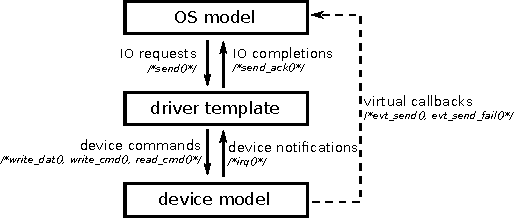
\includegraphics[width=0.85\linewidth]{imgs/actions.pdf}
    \caption{Input specifications for driver synthesis.  
    Labels in italics show interfaces from the running example
    (Figure~\ref{f:ex}).}\label{f:actions}
\end{figure}

The virtual interface between the device and the OS, shown with the dashed arrow in Figure~\ref{f:actions}, is used by the device model to notify the OS model about important hardware events, such as completion of I/O transactions and error conditions.  Methods of the virtual interface do not represent real runtime interactions between the device and the OS, but are used by the OS model to specify correctness constraints for the driver (see Section~\ref{s:virt}).

Finally, the driver template contains a partial driver implementation to be completed by \termite.  A minimal template consists of a list of driver entrypoints without implementation.  At the other extreme, it can provide a complete implementation, in which case \termite acts as a static verifier for the driver. By this we mean that it checks that the interactions between the driver software and the hardware ensure that all operating system requests are eventually fulfilled. It does not, for example, check for the absence of null pointer dereferences and similar defects that can be found by tools such as SLAM \cite{slam}. In fact, \tsl is designed to express state machines, not arbitrary programs and such defects are not expressible. Of course, this also limits the drivers that can be expressed.

All specifications are written using the \termite Specification Language (\tsl).  In line with our goal of making synthesis as close to the conventional driver development workflow as possible, \tsl is designed as a dialect of C with additional constructs for use in synthesis.  The full specification of the \tsl language is given in Appendix~\ref{ch:tsl_ref}. We introduce relevant features of \tsl throughout this section.

We minimize the amount of work needed to develop specifications for every synthesized driver by maximizing the reuse of specifications.  In particular, \termite allows the use of existing device specifications developed by hardware designers in driver synthesis.  It does this by providing a compiler from the modelling language used for the existing specification to \tsl. This is explained in Section~\ref{sec:device_model}.

Furthermore, the OS specification for the driver can be derived from a generic specification for a class of similar devices (e.g., network or storage).  Thus we expect that additional per-driver effort will consist of: 
\begin{enumerate}
    \item inserting device-class callbacks in appropriate locations of the device model and 
    \item extending the OS specification to support device-specific features missing in the  generic OS specification.
\end{enumerate}

\subsection{Device model}
\label{sec:device_model}

The device model simulates the device operation at a level of detail sufficient to synthesize a correct driver for it.  To this end, it must accurately model external device behavior visible to software.  At the same time, it is not required to precisely capture internal device operation and timing, as these aspects are opaque to the driver.

Such device models are routinely developed by hardware designers for the purposes of design exploration, simulation, and testing. They are widely used by hardware manufacturers in-house~\cite{cofluent} and are available commercially from major silicon IP vendors~\cite{vp}.  These models are known as \emph{transaction-level models} (TLMs) (in contrast to the detailed register-transfer-level models used in gate-level synthesis)~\cite{Cai_Gajski_03}.  A TLM focuses on software-visible events, or \emph{transactions}, such as a write to a device register or a network packet transmission.

While the transaction-level modeling technology is relatively new, TLMs are already widely used by hardware manufacturers in-house~\cite{cofluent} and are available commercially from major silicon IP vendors~\cite{vp}.  We are optimistic that in the future open-source TLMs will become commonplace, since a TLM does not expose internal implementation details of the device and is therefore less likely to expose sensitive IP.

Existing TLMs created by hardware designers can be used with minor modifications (explained in Section~\ref{s:virt}) for driver synthesis.  Model reuse dramatically reduces the effort involved in synthesizing a driver and is therefore crucial to practical success of driver synthesis.  By reusing an existing model, we also reuse the effort invested by hardware designers into testing and debugging the model throughout the hardware design cycle, thus making driver synthesis less susceptible to specification bugs.  Finally, since TLMs are created early in the hardware design cycle, TLM-based driver synthesis can be carried out early as well, thus removing driver development from the critical path to product delivery.

TLMs are written in high-level hardware description languages like SystemC and DML\@.  In order to use these models in driver synthesis, we need to convert them to \tsl.  This translation can be performed automatically, and we are currently working on a DML-to-\tsl compiler.  Since this work is not yet complete, device models used in the experimental section of this paper are either manually translated from existing TLMs or written from scratch using TLM modeling style guidelines~\cite{dml_ug}.

Unfortunately, few TLMs are publicly available at the moment, which means that driver synthesis must be performed by  device vendors in-house.  However this is likely to change in the future.  A TLM does not expose internal implementation details of the device and is therefore not part of sensitive IP\@.  At the same time, there exist strong incentives for manufacturers to make device TLMs available to third-party vendors to test their software and hardware products for compatibility with the given device.

\subsubsection{Running example}

\begin{figure}
\begin{tsllisting}[name=ex]
/* Device model */
template dev 

    /* Device internal state */
    uint8 reg_dat, reg_cmd, reg_status = 0; (*@\label{f:ex_dev:l:reg_decls}@*)

    /* device commands */
    controllable void write_dat(uint8 v) { (*@\label{f:ex_dev:l:start_access}@*)
        reg_dat = v; 
    };

    controllable void write_cmd(uint8 v) { 
        reg_cmd = v; 
    };

    controllable uint8 read_cmd() { 
        return reg_cmd; 
    };

    controllable uint8 read_status() { 
        return reg_status; 
    }; (*@\label{f:ex_dev:l:end_access}@*)

    /* internal behavior */
    process ptx { (*@\label{f:ex_dev:l:start_xmit}@*)
        forever {
            wait (reg_cmd == 1); (*@\label{f:ex_dev:l:wait}@*)
            choice {
                { 
                    os.evt_send(reg_dat); (*@\label{f:ex_dev:l:cb_succ}@*)
                    reg_status=0; 
                };
                { 
                    os.evt_send_fail(reg_dat);(*@\label{f:ex_dev:l:cb_fail}@*)
                    reg_status=1; 
                };
            };
            reg_cmd = 0;
            /*drv.irq(); (see Section 4)*/(*@\label{f:ex_dev:l:irq}@*)
        };
    }; (*@\label{f:ex_dev:l:end_xmit}@*)
endtemplate
\end{tsllisting}
\caption{Trivial serial controller device specifications.}
\label{f:ex_dev}
\end{figure}

Figure~\ref{f:ex_dev} shows a fragment of a model of a trivial serial controller device used as a running example.  The fragment specifies the send logic of the controller, which allows software to send data characters over the serial line.  The model is implemented as a \tsl \emph{template}.  The template encapsulates data and code that manipulates the data, similar to a class in OOP.

The software interface of the device consists of data, command, and status registers declared in line~\ref{f:ex_dev:l:reg_decls}.  The registers can be accessed from software via the \src{write\_dat}, \src{write\_cmd}, \src{read\_cmd}, and \src{read\_status} methods (lines~\ref{f:ex_dev:l:start_access}--\ref{f:ex_dev:l:end_access}).  The \src{controllable} qualifier denotes a method that is available to the driver and can be invoked from synthesized code.

The transmitter logic is modelled in lines~\ref{f:ex_dev:l:start_xmit}--\ref{f:ex_dev:l:end_xmit}.  It is implemented as a \tsl \emph{process}.  A \tsl specification can contain multiple processes.  The choice of the process to run is made non-deterministically by the scheduler.  The process executes atomically until reaching a \src{wait} statement or a controllable placeholder (see below).

In line~\ref{f:ex_dev:l:wait}, the transmitter waits for a command, issued by the driver by writing value $1$ to the command register.  Upon receiving the command, it sends the value in the data register over the serial line.  The transmission may fail, e.g., due to a serial link problem.  The device signals transmission status to software by setting the status register to $0$ or $1$.  Finally, it clears the command register, thus notifying the driver the request has completed.

Internally, the transmitter circuit consists of a shift register and a baud rate generator used to output data on the serial line.  These details are not visible to software and are abstracted away in the model.  We use the non-deterministic \src{choice} construct to choose between successful transmission and failure, without modelling the details of serial link operation.  Successful and failed transmissions are modelled using\src{evt\_send} and \src{evt\_send\_fail} events, explained in Section~\ref{s:os}.

\subsection{OS model}\label{s:os}

The OS model specifies the API mandated by the OS for all drivers of the given type.  For example, any Ethernet driver must implement the interface for sending and receiving Ethernet packets.  A separate specification is needed for each supported OS, as different OSs define different interfaces for device drivers.

A high degree of specification reuse can be achieved by  creating a library of generic specifications for common types of drivers, e.g., network, storage, or serial drivers.  A generic specification describes the API mandated by the OS for all drivers of the given type.  For example, any Ethernet driver must implement the interface for sending and receiving Ethernet packets.  A separate generic specification is needed for each supported OS, as different OSs define different interfaces for device drivers.

Additionally, each particular device can support non-standard features, e.g., device-specific configuration options or transfer modes.  These features must be added as extensions to the generic OS specification in order to synthesize support for them in the driver.  \tsl supports such extensions in a systematic way via the template inheritance mechanism.  This is described in Appendix~\ref{ch:tsl_ref}.

\subsubsection{Running example}

\begin{figure}
\lstset{firstnumber=last}
\begin{tsllisting}[name=ex]
/* OS model */
template os 

    uint8 dat;
    bool inprogress, acked, success; (*@\label{f:ex_os:l:vars}@*)

    /* driver workload generator */
    process psend {
        forever {
            dat = *; /*randomise dat*/ (*@\label{f:ex_os:l:nondet}@*)
            inprogress = true;
            acked = false;
            drv.send(dat);
            wait(acked); (*@\label{f:ex_os:l:wait}@*)
        };
    };

    /* I/O completions */
    controllable void send_ack(bool status) { (*@\label{f:ex_os:l:ack}@*)
        assert (!inprogress && !acked && status == success);
        acked = true;
    };

    /* virtual callbacks */
    void evt_send(uint8 v) { (*@\label{f:ex_os:l:send_cb}@*)
        assert (inprogress && v==dat); (*@\label{f:ex_os:l:assert}@*)
        inprogress = false; (*@\label{f:ex_os:l:inprogress}@*)
        success = true; (*@\label{f:ex_os:l:success}@*)
    };

    void evt_send_fail(uint8 v) {
        assert (inprogress && v==dat);
        inprogress = false;
        success = false;
    };

    /* The goal */
    goal idle_goal = acked; (*@\label{f:ex_os:l:goal}@*)
endtemplate
\end{tsllisting}
\caption{Trivial serial controller driver specifications.}
\label{f:ex_os}
\end{figure}

Figure~\ref{f:ex_os} shows the operating system model. It is written in the form of a test harness that simulates all possible sequences of driver invocations issued by the OS\@.  The \src{os} template in Figure~\ref{f:ex_os} shows the OS model for our running example.  The main part of the model is the \src{psend} process.  At every iteration of the loop, it non-deterministically chooses an 8-bit value (line~\ref{f:ex_os:l:nondet}) and calls the \src{send} method of the driver, passing this value as an argument.  It then waits for the driver to acknowledge the transmission of the byte (line~\ref{f:ex_os:l:wait}) before issuing another request.  The driver acknowledges the transmission via the \src{send\_ack} callback (line~\ref{f:ex_os:l:ack}).  The callback sets the \src{acked} flag, which unblocks the \src{psend} process.

We keep the specification concise by modeling the state of the driver-OS interface, as opposed to the internal OS state and behavior.  For example, the \src{acked} variable (line~\ref{f:ex_os:l:ack}) serves to model the flow of data between the OS and the driver and is not necessarily present in the OS implementation.

\subsection{Connecting device and OS models}
\label{s:virt}

In addition to simulating I/O requests to the driver, the OS model also specifies the semantics of each request in terms of device-internal events that must occur in order to complete the requested I/O operation.  In our running example, after the OS invokes the \src{send} method of the driver and before the driver acknowledges completion of the request, the device must attempt to send the requested data over the serial line.  This requirement establishes a connection between the device and OS models and must be specified explicitly in order to enable \termite to generate a driver implementation that correctly handles the OS request.  Note that we only need to specify \emph{which} hardware events must occur, but not \emph{how} the driver generates them.

In order to develop such specifications, we need a way to refer to relevant state and behavior of the device from the OS model.  At the same time, in order to maximize specification reuse, we would like to keep the OS specification device-independent.  To reconcile these conflicting requirements, we introduce a \emph{virtual interface} between the device and OS model.  This interface consists of callbacks used by the device model to notify the OS model about important hardware events.  The virtual interface does not represent real runtime interactions between the device and the OS, but serves as part of the correctness specification.

We define a virtual interface for each class of devices.  Such \emph{device-class} interfaces are both device and OS-independent.  The device-class interface can be extended with additional device-specific callbacks as required to specify a driver for a particular device.

\subsubsection{Running example}

\todo{device class source}

In our example, we define a device-class interface consisting of two virtual callbacks: \src{evt\_send} and \src{ev\_send\_failed}, invoked respectively when the device successfully transmits and fails to transmit a byte.  These callbacks are invoked in lines~\ref{f:ex_dev:l:cb_succ} and~\ref{f:ex_dev:l:cb_fail} of the device model.  The \src{evt\_send} handler is shown in line~\ref{f:ex_os:l:send_cb} of the OS model.  The assertion in line~\ref{f:ex_os:l:assert} specifies that the send event is only allowed to occur if there is an outstanding send request in progress and the value being sent is the same as the one requested by the OS\@.  We reset the \src{inprogress} flag to false in line~\ref{f:ex_os:l:inprogress}, thus marking the current request as completed; line~\ref{f:ex_os:l:success} sets the \src{success} flag to true, thus indicating that the transfer completed without an error.  The \src{evt\_send\_fail} handler is identical, except that it sets the \src{success} flag to false.  The flags are checked by the \src{send\_ack} method, which asserts that the driver is only allowed to acknowledge a completed request (\src{!inprogress}) that has not been acknowledged yet (\src{!acked}) and that the completion status reported by the driver must match the one recorded in the \src{success} flag.

In this example we use C-style assertions to rule out invalid system behaviors.  Assertions alone do not fully capture requirements for a correct driver behavior.  For example, a driver that remains idle does not violate any assertions.  Hence, we need to specify requirements for the driver to make forward progress.  We introduce such requirements into the model in the form of \emph{goal conditions}, that must hold \emph{infinitely often} in any run of the system.  For example, a goal may require that the driver is infinitely often in an idle state with no outstanding requests from the OS\@.  The OS can force the driver out of the goal by issuing a new I/O request.  To satisfy the goal condition, the driver must return to the goal state by completing the request.  Line~\ref{f:ex_os:l:goal} in Figure~\ref{f:ex_os} defines such a goal condition that holds whenever the \src{acked} flag is set, i.e., the driver has no unacknowledged send requests.

\subsection{Driver template}

\subsubsection{Running example}

\begin{figure}
\lstset{firstnumber=last}
\begin{tsllisting}[name=ex]
/* Driver template */
template drv 

    void send(uint8 v){ (*@\label{f:ex_drv:l:send}@*)
        ...; (*@\label{f:ex_drv:l:magic}@*)
    }; 

    /*
    void irq(){ (see Section 4) (*@\label{f:ex_drv:l:irq}@*)
        ...;
    }; 
    */
endtemplate
\end{tsllisting}
\caption{Trivial serial controller driver specifications.}
\label{f:ex_drv}
\end{figure}

Figure~\ref{f:ex_drv} shows the driver template for the running example consisting of a single \src{send} entry point invoked by the OS\@.  The ellipsis in line~\ref{f:ex_drv:l:magic} represent a location for inserting synthesized code and are part of \tsl syntax.  We refer to such locations as \emph{controllable placeholders}. 

\section{\tsl compiler}

In order to compute the most general driver strategy as a solution of a two-player game, we must first convert input \tsl specifications into a game automaton.  This conversion is performed by the \tsl compiler.

Real driver specifications have large state spaces, which cannot be feasibly represented by explicitly enumerating states, as in Figure~\ref{f:actions}.  Therefore, in \termite we represent games symbolically (Section~\ref{sec:symbolic_games}).  The state space of the game is defined in terms of a finite set of state variables $X$, with each state $s\in S$ representing a valuation of variables in $X$.  The \tsl compiler introduces a state variable for each \tsl variable declared in one of the input templates.  In addition, auxiliary state variables are introduced to model the current control location of each \tsl process.
        
We model controllable and uncontrollable actions as valuations of action variables $Y_c$ and $Y_u$.  Transition relations $\delta_c$ and $\delta_u$ are represented symbolically as formulas over state variables $X$, action variables $Y_c$ and $Y_u$, and next-state variables $X'$.  

The \tsl compiler splits the input specification into controllable and uncontrollable parts and translates them into controllable and uncontrollable transition relations respectively.  The controllable part is comprised of controllable methods that can be invoked by the driver.  The controllable transition relation $\delta_c$ is computed by rewriting controllable methods in the \emph{variable update form}.  Consider, for example, variable \src{reg\_dat} declared in line~2 in Figure~\ref{f:ex}.  This variable is only modified by the \src{write\_dat} method in line~4.  The corresponding fragment of the controllable transition relation in the variable update form is
%$$
%\mathtt{reg\_dat' := (tag=write\_dat)~?~v : reg\_dat}
%$$
$$
\small
\begin{aligned}
    &reg\_dat' = \begin{cases}
                     v       , & \text{if } tag=write\_dat \\
                     reg\_dat, & \text{otherwise},
                 \end{cases}\\
\end{aligned}
$$
where $\mathtt{reg\_dat'}$ is the next-state variable representing the value of $\mathtt{reg\_dat}$ after the transition. A special $tag$ variable is used to identify the method being invoked. For example, the specification in Figure~\ref{f:ex} has four controllable methods, so $tag$ can take one of the four values $write\_dat$, $write\_cmd$, $read\_status$ and $send\_ack$.  In addition, a separate variable is introduced for each argument of every controllable method ($v$ in this example). 

The uncontrollable part of the specification is comprised of \tsl processes, which model device and OS behavior.  We syntactically decompose each process into atomic transitions.  Recall that a process executes atomically until reaching a \src{wait} statement or a controllable placeholder.  Consider the \src{ptx} process in line~13 in Figure~\ref{f:ex}.  The process is initially paused in the wait statement.  It is scheduled to run when the wait condition holds.  It executes the statements in lines~16--22 atomically and stops again in line~15.  As part of this atomic transition, the process sets the \src{reg\_cmd} variable to 0 (line~22).  This is the only uncontrollable transition that modifies this variable, hence the uncontrollable update function for this variable is defined as follows:
%$$
%\mathtt{reg\_cmd' := (reg\_cmd=1 \land pid=ptx)~?~0 : reg\_cmd}
%$$,
$$
\begin{aligned}
    &reg\_cmd' = \begin{cases}
                    0       , & \text{if } reg\_cmd=1 \land pid=ptx\\
                    reg\_cmd, & \text{otherwise},
                 \end{cases}\\
\end{aligned}
$$
where $\mathtt{pid}$ is an uncontrollable action variable that models the scheduler's choice of a process to run, and the $\mathtt{reg\_cmd=1}$ conjunct corresponds to the wait condition in line~15.
  
Finally, we need to generate the game objective $\Phi$.  In a symbolic representation of the game, goal and fair sets are specified as conditions over state variables that hold for each state in the set.  The \tsl compiler outputs a goal set $B_i$ for each goal declared in the input specification and a fair set $F_i$ for each \src{wait} statement.  The latter guarantees that every runnable process gets scheduled eventually.
        
In addition to goal conditions, a \tsl specification also contains assertions, which must never be violated.  We model assertions using an auxiliary boolean state variable $\varepsilon$, which is set to true whenever an assertion is violated and remains true forever after.  We add an extra constraint $\varepsilon=false$ to each accepting set $B_i$.  An assertion violation permanently takes the game out of $B_i$, and therefore can not occur in any winning run of the game.

\section{User-guided code generation}
\label{s:user-guided}

The set of input \tsl specifications is fed into the \termite synthesis engine, which then automatically computes the most general strategy for the driver.  Given a state of the system, the most general strategy determines the set of all valid driver actions in this state.  The most general strategy is used by the \termite code generator to produce a driver implementation in C in a user-guide fashion.

\subsection{Motivation}

Early versions of \termite implemented fully automatic code generation as their only mode of operation.  In many cases we found that the tool produced unsatisfactory code, which led to a series of improvements to the code generation algorithm, aimed to generate more compact, user-readable, and efficient implementations.  At the same time, we found that many aspects of what is perceived by developers as a good implementation are very hard to formalize, and, even when possible, the effort involved in such a formalization exceeds the effort needed to achieve the desired effect manually.

For example, the interrupt handler logic of most drivers follows the standard structure, where the driver checks every interrupt source in the order of its priority and invokes a separate handler function for every signaled interrupt.  Interrupt prioritization and functional decomposition are hard to synthesize automatically without manual guidance.

One might argue that structure and readability are not relevant for synthesized code.  In practice, however, if synthesized drivers are to make their way into Linux and other major OSs, they must follow standard coding guidelines adopted by these OSs and be amenable to manual code inspection.  Furthermore, human readable code is needed for quality assurance.  While automatic synthesis guarantees that the synthesized driver is correct with respect to input specifications, it does not protect against specification defects: despite our best effort to maximize specification reuse and follow good modeling practices, specification defects cannot be avoided altogether.  Hence, manual inspection remains an important way to eliminate driver bugs.

In summary, while there exists a potential for further improvement of automatic code generation algorithms, we believe that a truly practical driver synthesis tool must put the user in control of the resulting code and not enforce any particular code structure nor attempt to override user's design decisions.

\subsection{Workflow}

The \termite code generator GUI is similar to a traditional integrated development environment with two additional built-in tools: the \emph{generator} and the \emph{verifier}.  The generator works as advanced auto-complete that helps the user to fill the controllable placeholders inside the driver template with code.  At any point, the user can invoke the generator to synthesize a single statement or a complete block of code inside a controllable placeholder via a mouse click on the target code location.  The user can arbitrarily modify and amend the generated code.  However, the generator never modifies user code.  Instead it tries to extend it to a complete implementation, which is always possible provided that the existing code is consistent with the most general strategy.  The generator currently only allows synthesizing statements after the last control location within a branch.  However this restriction is not a conceptual one and will be lifted by ongoing development.

The verifier automatically and on the fly checks that the driver implementation, comprised of a mix of generated and manually written code, is consistent with the most general strategy, thus maintaining strong correctness guarantees that one would expect in automatically synthesized code.  The verifier symbolically simulates execution of the system, following the partial driver implementation created so far, and signals the user whenever it encounters a transition that violates the most general strategy.

In the first approximation, the generator algorithm is quite simple: given a source code location, it determines the set of possible system states in this location, picks an action for each state from the most general strategy and translates this action into a code statement.  In practice the algorithm uses a number of heuristics to produce compact and human-readable code.  In particular, whenever there exists a common action in all possible states in the given location, the algorithm produces straight-line code without branching. These heuristics are described in Section~\ref{sec:heuristic_codegen}.

\subsection{Running Example}

When running the generator on our running example, it automatically generates the code in Figure~\ref{f:ex_gen_send} for the \src{send} function (line~\ref{f:ex_drv:l:send} of the device template, Figure~\ref{f:ex_drv}):

\begin{figure}
\begin{tsllisting}
void send(uint8 v){
    dev.write_dat(v);
    dev.write_cmd(1);
    wait(dev.reg_cmd==0);
    if (os.success) {
        os.send_ack(true);
    } else {
        os.send_ack(false);
    };
};
\end{tsllisting}
\caption{Generated \code{send} function}
\label{f:ex_gen_send}
\end{figure}

This implementation correctly starts the data transfer by writing the value to be sent to the data register and setting the command register to $1$.  It then waits for the transfer to complete, which is signalled by the device by resetting the command register to $0$.  Finally, it acknowledges the completion of the transfer to the OS.

Note that the generated code refers to the \src{dev.reg\_cmd} and \src{os.success} variables.  These variables model internal device and OS state respectively and cannot be directly accessed by the driver.  This example illustrates an important limitation of \termite---it assumes a white-box model of the system, where every state variable is visible to the driver.  Ideally, we would like to synthesize an implementation that automatically infers the values of important unobservable variables.  In this case, the value of the command register can be obtained by the driver by executing the \src{read\_cmd} action.  Furthermore, the value of the \src{os.success} variable is correlated with the completion status of the last transfer, which can be obtained by reading the device status register.

While \termite currently cannot produce such an implementation automatically, it implements a pragmatic tradeoff that helps the user build and validate a correct implementation with modest manual effort.  The code generator warns the user that the auto-generated code accesses  private variables of the device and OS templates.  This prompts the user to provide a functionally equivalent valid implementation, replacing the \src{wait} statement with a polling loop and using the \src{read\_status} method to check transfer status, as shown in Figure~\ref{f:ex_man_send}.

\begin{figure}
\begin{tsllisting}
void send(uint8 v){
    dev.write_dat(v);
    dev.write_cmd(1);
    (*@{\bf\ttfamily while(dev.read\_cmd()==1){};}@*)
    if ((*@\bf\ttfamily dev.read\_status()@*)) {
        os.send_ack(true);
    } else {
        os.send_ack(false);
    };
};
\end{tsllisting}
\caption{Manually written \code{send} function}
\label{f:ex_man_send}
\end{figure}

The verifier automatically checks the resulting implementation and confirms that it satisfies the input specification.

Note that in this example we have synthesized code that correctly handles device errors.  This was possible, as our input device specification correctly captures device failure modes (namely, transmission failure) and our OS specification describes how the driver must report errors to the OS (via the \src{status} argument of the completion callback).

In principle, it is also possible to synthesize a driver implementation that handles device and OS failures \emph{not} captured in the specifications: since the synthesis tool knows all possible valid environment behaviors, it can easily detect invalid behaviors and handle them gracefully.  Automatic synthesis of such \emph{hardened} device drivers is a promising direction of future research.

The final step of the code generation process translates the synthesized driver implementation to C.  This is a trivial line-by-line translation.  We expect this translation to become unnecessary in the future as our ongoing work on the \tsl syntax aims to make the synthesized subset of \tsl a strict subset of C.

\subsection{Maintaining synthesized code~~} 
Device driver development is not a one-off task: following the initial implementation, drivers are routinely modified toimplement additional functionality, adapt to the changing OS interface or support new device features.

The user-guided code generation method naturally supports such incremental maintenance. Since \termite uses \tsl as both its input and output language;  a completely or partially synthesized driver can be given as input to \termite, along with modified versions of the device and OS models.

A typical maintenance task proceeds in three steps:

\begin{enumerate}
    \item First, the developer amends device and OS models to reflect the new or changed functionality.  
    \item Second, they add new methods to the previously synthesized driver, if necessary, and replace existing driver code that is expected to change with a controllable  placeholder.  
    \item Finally, the user runs \termite to synthesize code for all controllable placeholders.  
\end{enumerate}
        
\termite treats all existing driver code as part of the uncontrollable environment.  Hence, if some of the old code is incorrect in the context of the new specifications, this will lead to a synthesis failure, and counterexample-based debugging is used to identify the faulty code, as described in Section~\ref{s:debug}.

\subsubsection{Running Example}

As an example, we synthesize a new version of the driver for our running example assuming a more advanced version of the serial controller device that uses interrupts to notify the driver on completion of a data transfer.  The new device model is obtained by uncommenting line~\ref{f:ex_dev:l:irq} of the device model in Figure~\ref{f:ex_dev}, which invokes the interrupt handler method of the driver after each transfer.  The driver template (Figure~\ref{f:ex_drv}) is extended with the \src{irq} method (line~\ref{f:ex_drv:l:irq}).  We use the previously synthesized implementation of the \src{send} method, but manually remove the last two lines, which implement polling, as we want the new implementation to use interrupts instead:

\begin{tsllisting}
void send(uint8 v){
    dev.write_dat(v);
    dev.write_cmd(1);}
\end{tsllisting}

Finally, we run \termite on the resulting specifications and use the generator to automatically produce the following implementation of the new \src{irq} method:

\begin{tsllisting}
void irq(){
    if (os.success) {
        os.send_ack(true);
    } else {
        os.send_ack(false);
    };}
\end{tsllisting}

As before, we manually replace the if-condition in the first line with

\begin{tsllisting}
if (dev.read_status())
\end{tsllisting}

This example illustrates how \termite supports incremental changes to the driver by reusing previously synthesized code, while maintaining strong correctness guarantees.

\subsection{Instrumenting synthesized code~~} 
\termite does not automatically instrument synthesized code for debugging, logging, accounting, etc.  However, the user can add such instrumentation manually.  \termite interprets such code as no-ops and, as with any manual code, never makes any modifications to it.

\section{Heuristic code generation}
\label{sec:heuristic_codegen}

Termite acts as an advanced auto-complete by suggesting lines of code for the driver. These suggestions are obtained using the symbolic strategy generated in the synthesis phase. Termite keeps track of the possible set of states that the system may be in at each line of code in the graphical IDE and uses this along with the strategy to generate a suggestion. 

Generating a winnng move from an individual state is straightforward. All one has to do is look up the state in the strategy relation and pick any winning label related to that state. Termite's code generator, however, deals in sets of states - the set of states which the system may be in at a particular line - which complicates matters considerably. For example, although every state in the set is winning (an invariant that the code generator enforces), there might not exist a single label that is winning for all of these states. In this case, the code generator uses smarter methods for picking labels or possibly falls back to spliting the current state set in two, as described in the following sections.

\subsection{Straightford label picking}

In the simplest case, there exists a winning action that is available from all states within the current line's state set (denoted $stateSet$). This action will cause all states in $stateSet$ to transition to a state closer to the goal, guaranteeing that if we keep choosing actions in this way we will eventually force execution into the goal. We compute the set of such winning actions using the formula in Equation~\ref{eqn:simple_strat}. 

\begin{equation}
\forall s. \: stateSet \rightarrow strategy
\label{eqn:simple_strat}
\end{equation}

This returns the set of labels which are part of the strategy for all states in the current state set. If the set is not empty, the Termite IDE the picks one of these at random as the autocompletion suggestion. If it is empty, the Termite IDE falls back to the more computationally expensive heuristic described in the next section.

\subsection{Smarter label picking}

While the above heuristic is straightforward and cheap, is it often unsatisfactory in practice. As an example, consider a current state set containing two states: $s_1$ and $s_2$. Suppose there is no label which is in the winning strategy for both states, but there is a label in the winning strategy for $s_1$ and it does not take $s_2$ further away from the goal. Such an action is a good candidate for an auto completion, however it will not be found by the first heuristic.

Our more general label picking algorithm works as follows: we find the greatest distance (N) of any state in $stateSet$ from the goal and then we look up two sets (which were computed and saved during synthesis).

\begin{itemize}
    \item the set of states at distance $N$, denoted $win_N$,
    \item and, the set of states at distance $N-1$, denoted $win_{N-1}$.
\end{itemize}

We define three constraints on the label, all computable symbolically, and pick a label that satisfies all three constraints by taking their conjunction, also symbolically.

When played, the label must:

\begin{itemize}
    \item keep execution in $win_{N-1}$ for states within $stateSet \cap win_{N-1}$, and
    \item keep execution in $win_N$ for states within $stateSet \cap win_N$, and
    \item take at least one state in $win_N$ into $win_{N-1}$.
\end{itemize}

These requirements ensure that each time a label is picked in this way, the number of states at the furthest distance to the goal decreases and eventually becomes zero as the number of abstract states in finite, in turn decreasing the maximum distance to the goal, $N$. Thus, repeatedly picking actions in this way ensures that we eventually get to the goal and is therefore a sound method of picking auto completions. Note that even though execution is guaranteed to reach the goal, the label picked may not be part of the strategy for all states in $stateSet$.

\subsection{Splitting states}

Lastly, suppose that there is no action found by the first two heuristics. In this case we recursively split $stateSet$ by finding a subset $a \subset stateSet$ from which there is a winning action for all of $a$ and splitting this out in C code using an \emph{if-statement}. What remains of $stateSet$ is recursively split enough times that there is a suitable label to play from each partition. This is guaranteed to eventually happen because $stateSet$ in finite. 

We describe how the condtion for this if-statement is computed. There exists at least one winning label from each state in the current set, as they are all winning. However, there does not exist a single label which is winning for all states in the current set. Our heuristic to find a subset of $stateSet$ for which there does exist such a label is as follows:

\begin{enumerate}
    \item Enumerate labels that are winning in some state in $stateSet$.
    \item Compute the set where each label is part of the strategy.
    \item Compute a small condition over state variables that distinguishes this set from the rest of $stateSet$.
    \item Choose the condition that is the simplest and return this and the corresponding lablel.
\end{enumerate}

\subsubsection{Enumerating winning labels}

In practice, the first step is infeasible, however. Games in Termite have labels over 100 bits in size so this would require enumerating over $2^{100}$ labels. However, many of these labels are equivalent as certain combinations of bits are dont-care. We use the $availableLabels$ algorithm (Algorithm~\ref{alg:available_labels}) to enumerate labels that are equivalent given the current set and transition relation.

This algorithm invokes two other algorithms: $genPair$ (Algorithm~\ref{alg:gen_pair}) and $enumerate$ (Algorithm~\ref{alg:enumerate}), both of which deserve some explanation. 

$genPair$, given two sets of variables ($X$ and $Y$) and a relation, extracts a single valuation of $X$ from the relation, determines the set of valuations of $Y$ that are related to and then determines the set of valuations of $X$ that relate to exactly this set. 

$enumerate$, given two sets of variables ($X$ and $Y$) and a relation repeatedly extracts pairs from the relation using $genPair$, erasing the $X$ valuations from the relation each time so that they are not chosen again. It computes a set of pairs of sets of $X$ and $Y$ valuations that are related to exactly the other element of the pair.

Finally, $availableLabels$ uses $enumerate$ to enumerate labels with different behaviours in the current $stateSet$. It does this by restricting the transition relation to transitions that originate from states in $stateSet$ and treating this as a relation between $\langle s, s' \rangle$ and $l$. This works because equivalent labels will result in the same $\langle s, s' \rangle$ relation, i.e.\ the same state transition, thus calling $enumerate$ with this relation and these variables will enumerate equivalent labels.

\begin{algorithm}
\begin{algorithmic}

\Function{GenPair}{$x$, $y$, $rel$}
    \State $xMinterm \gets \Call{extractMinterm}{\exists y. \: rel}$
    \State $img      \gets \Call{substitute}{rel, xMinterm}$
    \State $genX     \gets \forall y. \: reg \leftrightarrow img$
    \State\Return $\langle genX, img \rangle$
\EndFunction

\end{algorithmic}
\label{alg:gen_pair}
\end{algorithm}

\begin{algorithm}
\begin{algorithmic}

\Function{Enumerate}{$x$, $y$, $rel$}
    \State $result = []$
    \While{$rel \neq False$}
        \State $\langle genX, img \rangle \gets \Call{genPair}{x, y, rel}$
        \State $result \gets result \oplus \langle genX, img \rangle$
        \State $rel \gets res \land \neg genX$
    \EndWhile
    \State\Return $result$
\EndFunction

\end{algorithmic}
\end{algorithm}

\begin{algorithm}
\label{alg:enumerate}
\begin{algorithmic}

\Function{availableLabels}{$s, u, l, s', strategy, stateSet$}
    \State $winning \gets \exists \: s \: u \: s'. \: strategy \land stateSet$
    \State\Return$\Call{enumerate}{l, s \cup s', \delta \land stateSet \land winning}$
\EndFunction

\end{algorithmic}
\label{alg:available_labels}
\end{algorithm}

\subsubsection{Computing the condition}

We compute a condition over state variables that distinguishes the states where the label is winning from the rest using the $liCompaction$ function. This function, provided by the CUDD library, minimises a condition BDD given a care set so that it returns the correct value within the care set and is undefined otherwise. Our condition BDD is the set of states from the winning label is available and our care set is $currentState$. Since we are only applying the if condition in one of the states in $currentState$, this is the only set where it needs to be accurate. 

We found that a good heuristic is to choose the label which results in the simplest if condition, where a simple condition has a small BDD representation. The size of a BDD can be conveniently calculated using the function $dagSize$ from the CUDD library. 

\section{Counterexample guided debugging}
\label{s:debug}

An important practical issue in game-based synthesis is the complexity of diagnosing synthesis failures due to defects in the input specifications.  In the event that \termite fails to solve the game, the user needs to trace the failure back to the specification defect.  However, the failure does not carry any information about the defect, which makes the problem harder to resolve.

In \termite we propose a new approach to troubleshooting synthesis failures based on the use of \emph{counterexample strategies}.  A counterexample strategy is a strategy on behalf of the environment that prevents the driver from winning the game.  It is obtained by solving the \emph{dual game}, where, in order to win, the environment must permanently force the game out of one of the goal regions.  A winning strategy in the dual game is guaranteed to exist whenever solving of the primary game fails.

By exploring the counterexample strategy, the user can identify the defect in the input specification.  This is similar to the use of counterexamples in software verification, where for each discovered bug the verification tool generates a counterexample trace that triggers the bug.  However, a counterexample strategy cannot in the general case be represented by a single execution trace, as the choice of spoiling moves for the environment depends on the actions performed by the driver.

In order to detect and fix the defect in an input specification, the driver developer relies on their  understanding of the OS and device logic.  The role of the counterexample strategy is to guide the developer towards the defect.  To automate this process, we developed a powerful visual debugging tool that allows the user to interactively simulate intended driver behavior and observe environment responses to it.  The user plays the game on behalf of the driver, while the tool responds on behalf of the environment, according to the counterexample strategy.
 
In a typical debugging session, the debugger, following the counterexample strategy, generates a sequence of requests that are guaranteed to win against the driver.  The user plays against these requests by specifying device commands that, they believe, represent a correct way to handle the request.  Since this sequence of requests \emph{cannot} be handled correctly given the current input specification, at some point in the game the user runs into an unexpected behavior of one of the players, e.g., one of the user-provided commands does not change the state of the device as expected or the environment performs an uncontrollable transition that violates an assertion.  Based on this information, the user can revise the faulty specification.

At every step of the interactive debugging session, the debugger either chooses a spoiling uncontrollable action based on the counterexample strategy or, if the system is inside a controllable placeholder, allows the user to choose a controllable action to execute on behalf of the driver.  In the former case the spoiling uncontrollable action corresponds to a transition in one of the \tsl processes.  The user can explore this transition by stepping through it, exactly as they would in a conventional debugger.  In the latter case, the user provides the action that they would like to perform by typing and executing corresponding code statements.

The tool supports a number of features aimed at making the debugging process as simple as possible for the user. We mention two of them here: 
\begin{itemize}
    \item First, the debugger interactively prompts actions available to the driver at each step.  
    \item Second, the debugger keeps the entire history of the game and allows the user to go back to one of previously explored states and try a different behavior from there.
\end{itemize}

\section{Limitations}\label{s:limitations}

The core of a device driver entails translating I/O requests from the OS into sequences of low-level device commands and responses. We focus on synthesizing driver logic that performs these functions, and this is where game-based synthesis really shines, as it helps to implement tedious and error-prone logic with minimal manual effort and without bugs. However, there are several real world aspects of device driver creation that are not handled as gracefully by the game based approach.

In Section~\ref{s:user-guided}, we described one limitation of \termite, namely the lack of support for grey-box synthesis.  In this section we discuss other limitations, which, we hope, will help define the agenda for continuing research in driver synthesis.

\subsection{Direct Memory Access}

Most importantly, \termite does not currently support automatic synthesis of direct memory access (DMA) management code.  Many modern devices transfer data directly to and from main memory, where it is buffered in data structures such as circular buffers and linked lists.  These data structures can have very large or infinite state spaces and cannot be easily modeled within the finite state machine-based framework of \termite.  Efficient synthesis for DMA requires enhancing the synthesis algorithm to use a more compact representation of DMA data structures, which is the focus of our ongoing research.  At this time, code for manipulating DMA data structures must be written manually.  This code is not interpreted or verified by \termite.  For example, we use this approach to synthesize a DMA-capable IDE disk driver (Section~\ref{s:eval}).

\subsection{Boilerplate Code}

Device drivers in modern OSs contain a significant amount of boilerplate code that is not directly related to the task of controlling the device.  This includes binding the driver to I/O resources (memory mapped regions, interrupts, timers), registering the driver with various OS subsystems, allocating DMA memory regions, creating sysfs entries, etc.  While much of this functionality could be synthesized within the game-based framework, we do not believe that this is the correct approach.  Previous research has demonstrated that this boilerplate code can be generated in a principled way from declarative specifications of the driver's requirements and capabilities~\cite{Spear_RHHL_06}.  This technique has lower computational complexity than game solving and better captures the essence of the task.  A practical driver synthesis tool can combine game-based synthesis of the core driver logic responsible for controlling the device with declarative synthesis of boilerplate code.  As a result, the current version of \termite assumes this boilerplate code is written manually as a wrapper around the synthesized driver.

\subsection{Concurrency}

Drivers execute in a concurrent OS environment and must handle invocations from multiple threads, as well as asynchronous hardware interrupts.  We separate synthesis for concurrency into a separate step.  Drivers synthesized by \termite are correct assuming a sequential environment, where driver entry points are invoked atomically.  The resulting sequential driver is then processed by a separate tool that performs a sequence of transformations of the driver source code, which preserve the driver's sequential behavior, while making the driver thread-safe.  Such transformations include adding locks around critical code sections, inserting memory barriers, and reordering instructions to avoid race conditions.  Concurrency synthesis is still work in progress and is not the subject of this thesis.  Preliminary results are published in~\cite{Cerny_HRRT_13, Cerny_HRRT_14}.

\subsection{Real time synthesis}

\termite does not explicitly support specification and synthesis of timed behaviors.  Instead, it uses a pragmatic approach that allows it to synthesize time-sensitive behavior without having to explicitly reason about time.  To this end, \termite conservatively approximates timed operations by fairness constraints: it ignores the exact duration of each device operation, but keeps the knowledge that the operation will complete \emph{eventually}, and synthesizes a driver that waits for the completion.  \termite is also able to handle time-out conditions, modeled as external events.  However, at this time it is not capable of generating device drivers for hard real-time systems, where the driver must guarantee completion of I/O operations by a certain deadline.

\section{Implementation}

We implemented all components of the Termite toolkit, including the TSL compiler, the game solver, the counterexample debugger, the user-guided code generator, and the TSL-to-C compiler, in the Haskell programming language.  Our implementation uses the CUDD BDD library for efficient symbolic manipulations over boolen relations, and the Z3 SMT solver for satisfiability queries over the theory of bit vectors, as described in~\cite{Walker_Ryzhyk_14}.  Termite is publicly available under the BSD license and can be downloaded from the project website \texttt{\url{http://termite2.org}}. The version of \termite presented here consists of 30,000 lines of code.  The estimated overall project effort is 10 person years. 

\section{Evaluation}
\label{s:eval}
We evaluate \termite by synthesizing drivers for eight I/O devices.  Specifically, we synthesized drivers for a UVC-compliant USB webcam, the 16550 UART serial controller, the DS12887 real-time clock, and the IDE disk controller for Linux, as well as bare metal drivers (which, for example, would run on seL4~\cite{Klein_EHACDEEKNSTW_09}) for I2C, SPI, and UART controllers on the Samsung exynos 5 chipset\footnote{At the time of writing, the exynos drivers have not yet been tested due to hardware availability issues; however we confirmed via manual inspection that they implement the same device control sequences as existing manually developed drivers.} and SPI controller on the STM32F10 chipset.  With the exception of the IDE disk, these devices are representative of peripherals found in a typical embedded platform, such as a smartphone.  Our synthesized drivers implement data transfer, configuration and error handling.  The main barrier to synthesizing drivers for more advanced devices, e.g., high-performance network controllers, is the current lack of support for synthesis of DMA code in the current version of \termite.  

\subsection{Modelling complexity} 
Models of UART and DS12887 devices were developed based on existing publicly available device models~\cite{ds12887, uart}.  Models of other devices were derived from their vendor-provided documentation, following standard TLM modeling guidelines~\cite{dml_ug}.  OS models for the relevant device classes were created based on Linux kernel documentation and source code.  

Table~\ref{t:size} summarises the size, in lines of code, of device and OS models in our case studies.  Developing a complete set of specifications for each driver took approximately one week, of which only one to three days were spent building the models and the rest of the time was spent studying device and OS documentation.  This efficiency can be attributed to the choice of the right level of abstraction and modeling language.  In particular, the use of transaction-level device modeling abstracts away complicated internal device machinery by focusing on high-level events relevant to driver synthesis, while the \tsl language allows modeling the driver environment using standard programming techniques, as illustrated by our running example.

\begin{table}
    \begin{minipage}{\linewidth}
    \center
    %\begin{tabular}{|p{0.15\linewidth}|p{0.15\linewidth}p{0.15\linewidth}|p{0.15\linewidth}p{0.15\linewidth}|}
    \begin{tabular}{|l|c|c|c|c|}
        \hline
%        & \multicolumn{4}{|c|}{size (lines of code)} \\
%        \cline{2-5}
        & \multicolumn{2}{|c|}{input spec} & \multicolumn{2}{c|}{driver} \\
        \cline{2-5}
                     & OS  & device & synthesized & native \\
        \hline
        \hline
        webcam       & 102 & 385    & 113         & 307 \\
        16450 UART   & 122 & 167    & 74          & 261 \\
        exynos UART  & 128 & 252    & 37          & 166 \\
        STM SPI      & 73  & 244    & 24          & 64  \\
        exynos SPI   & 88  & 239    & 40          & 183 \\
        exynos I2C   & 146 & 180    & 79          & 211 \\
        RT clock     & 118 & 252    & 84          & 183 \\
        IDE          & 188 & 480    & 94\footnote{Excluding 36 lines of manually written code that manipulates the DMA descriptor table.} & 474 \\
        \hline
    \end{tabular}
    \end{minipage}
    \caption{Size (in lines of code) of input specifications and of synthesized and equivalent manually written drivers.}
    \label{t:size}
\end{table}

Interestingly, we found the most error-prone step in developing specifications for driver synthesis to be defining correct relative ordering of OS-level and device-level events with the help of the virtual interface (Section~\ref{s:virt}).  Na\"ive specifications tend to be either too restrictive, leading to synthesis failures, or too liberal, leading to incorrect synthesized drivers. As we gained more experience synthesizing different types of drivers, we identified common modeling patterns that help avoid errors in virtual interface specifications.  

As a common example, most virtual interfaces contain callbacks that signal a change to one of the device configuration parameters, e.g., transfer speed, parity, etc.  A na\"ive OS model may only allow such a callback to be triggered when the OS has requested a change to the corresponding device setting.  However, many devices only allow setting multiple configuration parameters simultaneously, so that setting any individual parameter triggers multiple callbacks, thus making the specification non-synthesizable.  The problem can be rectified by changing the device specification to only trigger callbacks if the new value of the parameter is different from the old one; however this bloats the device model due to the extra checks.  A better solution, used in all our models, is to design the OS specification to allow configuration callbacks to be triggered at any time, provided that the new value of the parameter is equal to the last value requested by the OS. 

\subsection{Synthesis time} 
Table~\ref{t:perf} summarises the performance of the \termite game solver in our case studies.  The second column of the table characterises the complexity of the two-player game constructed by the \tsl compiler from the input specifications in terms of the number of states variables and the total number of bits in these variables.  The third column shows the number of iterations of the abstraction refinement loop required to solve the game.  The next column shows the size of the abstract game at the final iteration, in terms of the number of predicates in the abstract state space of the game.  These results demonstrate the dramatic reduction of the problem dimension achieved by our abstraction refinement method.  The second-last column shows that the \termite game solver was able to find the most general winning strategy within a few minutes in all case studies.

\begin{table}
    \center
    \begin{tabular}{|l|ccccc|}
        \hline
                       & \multirow{2}{*}{vars(bits)} & refine- & predi- & synt.     & verif.   \\
                       &                             & ments   & cates  & time (s)  & time (s) \\
        \hline
        \hline
        webcam         & 128 (125565)                & 47      & 192    & 215       & 794 \\
        16450 UART     & 81  (407)                   & 65      & 128    & 210       & 464 \\
        exynos UART    & 80  (1185)                  & 54      & 111    & 645       & 82 \\
        STM SPI        & 68  (389)                   & 29      & 63     & 67        & 31 \\
        exynos SPI     & 83  (933)                   & 31      & 72     & 25        & 44 \\
        exynos I2C     & 65  (303)                   & 21      & 56     & 45        & 96 \\
        RT clock       & 92  (810)                   & 25      & 74     & 56        & 127 \\
        IDE            & 114 (1333)                  & 42      & 105    & 285       & 778 \\
        \hline
    \end{tabular}
    \caption{Performance of the \termite game solver.}
    \label{t:perf}
\end{table}

We compared the performance of the \termite game solver against a state-of-the-art abstraction refinement algorithm for games~\cite{Alfaro_Roy_07} as well as against the standard symbolic algorithm for solving games without abstraction~\cite{Piterman_PS_06}.  In all case studies, the \termite solver was the only one to find a winning strategy within a two-hour limit.  We refer the reader to~\cite{Walker_Ryzhyk_14} for a more detailed performance analysis of the \termite synthesis algorithm.

The final column of Table~\ref{t:perf} shows the time that it took \termite to verify a complete driver.  Recall that the \termite synthesis algorithm doubles as a verification algorithm and can be used to verify drivers written in \tsl.  We used complete synthesized drivers containing a combination of manual and automatically generated code as inputs to \termite.  We have been able to successfully verify all of our drivers.  We also experimented with introducing faults to synthesized drivers.  \termite was able to detect these faults and produce correct counterexample strategies.  In most cases verification took longer than synthesis.  The reason for this is that \termite has not yet been optimized for verification workloads.  This is one area for future improvement.

%\termite is the first synthesis tool based on abstraction 
%refinement, so we cannot compare it against other 
%abstraction-based algorithms.  We benchmark \termite against a 
%highly optimized implementation of the state of the art algorithm 
%for solving GR-1 games (without abstraction) by Piterman et 
%al.~\cite{Piterman_PS_06}.  This algorithm was not able to solve 
%any of our case studies within a two-hour time limit.  We 
%therefore produced a simplified version of the IDE case study with 
%only 75 state bits (instead of 1333 in the original 
%specification), which the Piterman et al. algorithm solved in 
%57 minutes.  For comparison, \termite solved this simplified 
%example in under 1 second.

\subsection{User-guided code generation and debugging} 
We evaluate the key contribution of this paper, namely the user-guided debugging and code generation technique.  Each line of code in a \termite-generated driver originates from one of three sources: it can be 
\begin{enumerate} 
    \item synthesized automatically by the tool, 
    \item developed offline and given to \termite as part of the driver template, or 
    \item added or modified by the user during an interactive code generation session.  
\end{enumerate}
A perfect synthesis tool, capable of generating a complete driver fully automatically while producing code that meets all non-functional requirements, would eliminate the need for manual code altogether.  We do not believe that such a tool is feasible in the near future.  We therefore explore the tradeoffs that arise when using our current, imperfect, tool.  In particular, we would like to empirically characterize situations when the user can rely on the synthesizer to automatically produce near-optimal code, and when they are better off completely or partially implementing certain functionality manually.  These tradeoffs are likely to change as the tool improves.

Based on our experience so far, automatic synthesis is most helpful in generating code that performs device configuration or starts a data transfer.  This code may involve a long sequence of commands to the device, which must be issued in the right order and with correct arguments.  The synthesis algorithm of \termite proved more effective at doing this than human developers, producing correct code that only requires minimal cosmetic changes in most cases.  For example, Figure~\ref{f:screenshot_write} shows a screenshot of \termite with a synthesized implementation of the IDE driver \src{write()} function, which starts a data transfer to the device.  The function writes request parameters into appropriate device data registers and sets bit fields in command registers to prepare the device for data transfer.  One deficiency in this auto-generated implementation is that it uses absolute values instead of symbolic constants for bit fields.

As another example of suboptimal synthesized code, consider the following synthesized fragment:

\vspace{5mm}
\begin{tsllisting}
void packet_received() {
    if (((packet_data[9:9] == 1) && (packet_data[14:14] == 1))) {
        os.ack_packet(1,1,packet_data[16:32]);
    } else if ((dev.packet_data[9:9] == 1)) {
        os.ack_packet(1,0,packet_data);
    } else if ((dev.packet_data[14:14] == 1)) {
        os.ack_packet(0,1,packet_data[16:32]);
    } else {
        os.ack_packet(0,0,packet_data[16:32]);
    };
};
\end{tsllisting}
\vspace{3mm}

which can be replaced by an equivalent one-liner:

\vspace{5mm}
\begin{tsllisting}
os.ack_packet(packet_data[9:9],
    packet_data[14:14],packet_data[16:32]);
\end{tsllisting}
\vspace{5mm}

\noindent While both issues can, and will, be addressed by an improved code generation algorithm, our experience shows that unaccounted corner cases will arise occasionally.  Therefore, the ability to manually modify synthesized code without sacrificing correctness is crucial for a practical synthesis tool.

Limitations of \termite are most noticeable in synthesizing interrupt handler code responsible for processing I/O completions.  This involves querying device state to determine which operations completed and with what status, reporting results to the OS, and clearing interrupt status registers.  Since \termite does not support grey-box synthesis, it can not generate this code automatically and instead produces code that directly accesses device-internal state (see Section~\ref{s:user-guided}).  \termite correctly reports such situations and allows the user to mitigate them by manually editing synthesized code.  In practice, however, we found it easier to develop most of the interrupt handler logic offline, as part of the driver template, and rely on \termite to (a) establish correctness of this code and (b) extend it to a complete implementation.

\begin{figure}
    \center
    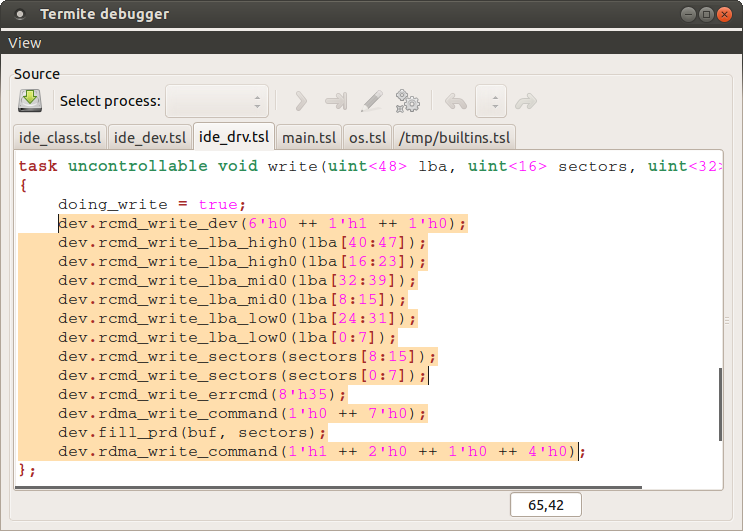
\includegraphics[width=\linewidth]{imgs/screenshot_write.png}
    \caption{Screenshot of \termite with a synthesized implementation of the IDE driver.  Automatically generated code is highlighted.}
    \label{f:screenshot_write}
\end{figure}

In our case studies, 60\% to 90\% of the code was generated fully automatically, with the rest of the code produced in a user-guided fashion.  Once an initial version of device and OS specifications was ready, it took us several hours to generate the driver implementation for each of our case studies.  Three quarters of this time was spent debugging the input specifications, with the rest of it spent generating driver source code with the help of the user-guided code generation GUI.

We found counterexample-driven debugging to be crucial to the productivity of synthesis-based development.  Before the debugger was available, we had to rely on code inspection to identify defects in the input specifications, which proved to be a frustrating and unpredictably long process.  The \termite debugger streamlines this process, giving us the confidence that any failure can be localised by following well-defined steps.  A typical debugging session takes a few minutes and involves entering only a few commands manually before the defect is localised. 

%We found the incremental approach to debugging and synthesis to 
%be the most effective.  Incremental synthesis 
%
%synthesise a single driver function or a small group of related 
%functions before adding m
%
%This is achieved by disabling invocations of all but one I/O 
%operations in the OS model. 
%
%Incremental synthesis

%In all case studies, we have been able to achieve human-readable 
%code structure that one would expect in a manually developed 
%driver.  60\% to 90\% of the code was generated fully 
%automatically and did not require any manual changes.  The rest of 
%the code was produced in a user-guided fashion, as described in 
%Section~\ref{s:user-guided}.  Human involvement was required for 
%three reasons.  First, it was necessary to get around the 
%white-box assumption, causing automatically generated code to 
%access variables outside the syntactic scope of the driver, as 
%explained in Section~\ref{s:user-guided}.  Second, it was used to 
%enforce a particular preferred implementation among several 
%functionally equivalent alternatives.  A common example of such a 
%situation, illustrated in Section~\ref{s:user-guided}, is 
%implementing I/O completions using interrupts instead of polling.  
%Finally, we relied on manual intervention to improve the structure 
%of synthesized code to make it compliant with the standard Linux 
%driver structure.

\subsection{Size of synthesized code} 
The last two columns of Table~\ref{t:size} compare the size of synthesized drivers to existing manually developed drivers.  Synthesised drivers are significantly more compact than conventional drivers for two main reasons.  First, as explained in Section~\ref{s:limitations}, we only synthesize the driver logic directly responsible for controlling the device.  Conventional drivers typically contain a large amount of boilerplate code managing various OS resources.  We believe that this code can and should be synthesized using complementary techniques.  At the moment we implement this functionality manually as a wrapper around the synthesized driver. 

Second, conventional device drivers are often designed to support multiple similar devices with slightly different interfaces and capabilities.  This leads to code bloat, as the driver must implement multiple versions of various operations, as well as logic to dynamically discover device capabilities and choose the right implementation to use.  In contrast, every \termite driver supports one specific device model with a fixed set of features.  Drivers for similar devices can share common specification code, but are synthesized as separate source code modules.  This approach leads to simpler code and is preferable for platforms with a fixed set of peripheral devices, such as smartphones, where shipping drivers that support only the required devices enables smaller system image.
  
\subsection{Specification reuse}  
Our specification methodology ensures mutual independence of device and OS specifications, and thus facilitates their reuse.  We have not yet carried out a substantial evaluation of such reuse; however we report our limited experience based on synthesizing two SPI drivers for the seL4 OS\@.  The corresponding OS specification was initially developed during the work on the SPI driver for the exynos chipset.  It was later used to synthesize a driver for the STM32F10 chipset.  We were able to reuse most of the original specification.  Minor changes (8 lines of code) were required in the part of the specification describing configuration functionality of the driver, since the STM SPI controller supports a number of ad hoc transfer modes.  We expect to observe similar pattern for other devices and operating systems: generic OS specifications can be reused with localized, device-specific changes required to support non-standard device features.

\subsection{Performance of synthesized drivers} 
Our synthesized drivers implement effectively identical device control logic to their conventional counterparts and therefore have similar performance.  We benchmarked the USB webcam driver, which is the most performance-critical one among our case studies.  We measured CPU load and data throughput generated by the conventional and synthesized drivers for varying bitrates.  We obtained identical results, modulo measurement errors, for both drivers in all cases.



\appendix
\chapter{TSL Language Reference}

\chapter{TSL Language Reference}
\label{ch:tsl_ref}

\hrule
\vspace{10pt}
\begin{center}
The design and implementation of the TSL language and its compiler were performed by Dr. Leonid Ryzhyk. This language reference is included here for completeness.
\end{center}
\hrule
\vspace{20pt}

\section{Overview}

\subsection{Static and dynamic namespaces}\label{s:o:namespace}

\tsl supports two namespaces: the \emph{static namespace} and the 
\emph{dynamic namespace}.  The static namespace is populated with 
compile-time objects: \emph{types} and \emph{constants}.  The 
dynamic namespace is populated with runtime objects: 
\emph{processes}, \emph{variables}, \emph{methods}, and 
\emph{wires}.  Static objects are uniquely identified by their 
name and syntactic scope.  In contrast, runtime objects can be 
instantiated multiple times within the specification and hence 
must be referred to relative to their runtime scope.  

\subsection{Templates}\label{s:o:templates}

Templates are the principal mechanism for managing both static and 
dynamic namespaces.  A template models an entity, such as a 
device, an OS, or a device driver.  It declares a set of static 
objects (types and constants) and a set of runtime objects.  
Static objects declared inside a template can be referenced from 
any part of the specification via the template name.  Runtime 
objects are instantiated together with the template and can be 
accessed via a reference to a template \emph{instance}.

The following template declares type \src{word} (static object) 
and variable \src{x} (runtime object):
\begin{tsllisting2}
template A
  // type declaration
  typedef uint<16> word;
  // variable declaration
  export word x;
endtemplate
\end{tsllisting2}
The \src{word} type is globally visible via the \src{::}-notation 
as \src{A::word}.  It can be used even if template \src{A} is 
never instantiated.  In contrast, variable \src{x} can only be 
accessed via an instance of \src{A}.  

A template is instantiated inside another template.  The only 
exception is the \src{main} template, which is implicitly 
instantiated in the top-level scope.  Every complete \tsl 
specification must contain a template called \src{main}.  

In the following example, the \src{main} template creates an 
instance of \src{A}, making its variables accessible from 
\src{main} via instance name:
\begin{tsllisting2}
template main
  instance A a;

  process pmain {
    // assigning variable x of template instance a.
    a.x = 16'd0;
  }
endtemplate
\end{tsllisting2}

The template instantiation mechanism gives rise to an 
\emph{instance tree} with the \src{main} template as its root.  
Dynamic objects within the tree are accessed using hierarchical 
identifiers such as \src{a.x}.  This mechanism allows accessing 
objects down the branch of the instance tree, starting at the 
local template.  In practice, it is often necessary to access 
objects instantiated in other parts of the tree.  This is achieved 
in a structured way using \emph{template ports}.  

A template port is an alias to a template of a given type bound at 
the time of instantiation.  For example, template \src{B} below 
declares port \src{aa} of type \src{A}, which makes runtime 
objects in the scope of \src{A} visible from \src{B}.  Both 
templates are then instantiated in the \src{main} template, with 
the instance of \src{A} connected to port \src{aa} of \src{B}.
\begin{tsllisting2}
// template B with port aa of type A
template B(A aa)
  process proc {
    aa.x = 16'd0;
  };
endtemplate

template main
  // create instances of A and B; connect port aa of
  // B to the instance of A.
  instance A a;
  instance B b(a);
endtemplate
\end{tsllisting2}

The following diagram illustrates the resulting instance tree and 
the link between different branches of the tree via port \src{aa}.

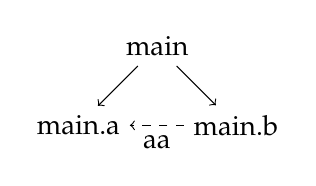
\begin{tikzpicture}
    \node[rectangle] (m) at (0,1) {main};
    \node[rectangle] (a) at (-1,0) {main.a};
    \node[rectangle] (b) at (1,0) {main.b};
    \path[->] (m) edge (a);
    \path[->] (m) edge (b);
    \path[->,dashed] (b) edge node[auto]{aa} (a);
\end{tikzpicture}

Another mechanism for managing name spaces is \emph{template 
inheritance}.  Using inheritance, one can create generic templates 
that capture common properties of a family of entities, leaving 
some of the properties underspecified.  The generic template can 
be specialised by a child template that fills in the missing 
details.  For example, the following template models common 
device-class callbacks that must be implemented by any OS 
specification for the IDE device class.  Note that callbacks are 
defined without bodies, as the exact behaviour is OS-specific.
\begin{tsllisting2}
template ide_os
  procedure void write_sectors(uint<48> lba, 
    uint<16> sectors, uint<32> buf, bool xfer_error);
  procedure void read_sectors(uint<48> lba, 
    uint<16> sectors, uint<32> buf, bool xfer_error);
  procedure void reset();
  ...
endtemplate
\end{tsllisting2}
This template is specialised by the \src{l4\_ide\_os} template,
that describes the IDE driver interface defined by the seL4 OS.
\begin{tsllisting2}
template l4_ide_os(l4_ide_drv drv)
  // the derive statement is used to establish the 
  // inheritance relation
  derive ide_os;

  // additional specification items can be declared in the 
  // child template
  export iostatus reset_status = ionone;

  // the child template implements methods inherited from 
  // the parent.
  procedure void write_sectors(uint<48> lba, 
    uint<16> sectors, uint<32> buf, bool xfer_error)
  {
    assert (lba == r_lba);
    ...
  }
\end{tsllisting2}

A template that has part of its functionality, namely method body 
or wire assignment, underspecified is called \emph{pure template}.  
Pure templates can be used in derive statements and in port 
declarations, however they cannot be instantiated.

Template inheritance is subject to the following rules:
\begin{itemize}
    \item Derived template must re-declare all ports of all its 
        parent templates with the same names and types.  It can 
        also declare additional ports not found in any of its 
        parents.

    \item If a template has multiple parent templates, then the 
        namespaces of parent templates (consisting of variable, 
        wire, method, goal, and process names) must not overlap.

    \item If the derived template re-declares a wire or method 
        declared in one of its parents, the new declaration must 
        have the same signature as the parent declaration.

    \item The child template can override wire and method 
        declarations of its parent templates.  Other parts of the 
        parent template, including variable, goal, and process 
        declarations, are inherited by the child template and 
        cannot be overriden.
\end{itemize}



\subsection{Execution model}\label{s:o:execmodel}

All state transitions in \tsl occur in the context of 
\emph{processes}.  Multiple processes can be enabled at the same 
time; however exactly one process participates in each individual 
transition.  Process transitions are atomic with respect to other 
processes.  Process that perform the next transition is chosen by 
the scheduler among enabled processes.  Scheduling is fair, i.e., 
if a process stays enabled sufficiently long, it will eventually 
get scheduled.

Processes are declared inside templates using the \src{process} 
keyword.  Such processes become runnable in the initial state of 
the specification.  Additional processes can be spawned at runtime 
using the \src{fork} construct.  Syntactic constraints of the 
language (namely, the lack of support for recursion) guarantee 
that only a bounded number of processes can be spawned at any 
time.  

In the following example, template \src{A} contains a single 
static process \src{psndrcv}, which spawns two subprocesses 
\src{psend} and \src{preceive}.
\begin{tsllisting2}
template A

process psndrcv {
  fork {
    psend:    forever send();
    preceive: forever receive();
  };
  shutdown();
};
...

endtemplate
\end{tsllisting2}

%In addition to statically and dynamically created processes, every 
%\tsl specification contains an implicit \emph{idle} 

A process state transition starts in the current program location 
and stops at the next \emph{pause location}.  Pause locations can 
be explicit or implicit.  Explicit pause locations are declared 
using \src{pause}, \src{wait}, and \src{stop} constructs.  
Implicit pause locations are introduced automatically by the 
compiler in the following cases:

\begin{itemize}
    \item Before \src{fork} statements
    \item Before magic blocks~\ref{s:o:magic}
    \item On entries to and exits from controllable and 
        uncontrollable tasks (see below)
\end{itemize}

Process behaviour can be factored into \emph{methods}.  A process 
can invoke methods declared inside its own template as well as in 
other template instances, via hierarchical identifiers discussed 
in the previous section.  There are three types of methods in 
\tsl: \emph{functions}, \emph{procedures}, and \emph{tasks}.  
Functions and procedures must complete instantaneously, i.e., they 
are not allowed to contain explicit or implicit pauses.  In 
addition, functions are not allowed to have side effects, i.e., 
they cannot modify any global variables, perform pointer 
dereferences, or contain assertions (pointer dereferences and 
assert statements can have the side effect of taking the system 
into an error state).  

Tasks can take time to execute.  A task can have an optional 
\src{controllable} or \src{uncontrollable} qualifier.  
Controllable tasks are the only kind of task that can be invoked 
from synthesised code; although they can also be called from 
manually written code.  They are used to model the device register 
interface and OS callbacks.  In the current implementation of the 
\tsl compiler, controllable tasks are subject to additional 
constraint: they are not allowed to contain internal pause 
locations, i.e., a controllable task must always complete in a 
single transition. 

Uncontrollable tasks represent driver methods invoked by the OS or 
the device.  Uncontrollable tasks are the only kind of task that 
can contain automatically generated code, i.e., a magic block can 
only be placed inside an uncontrollable task.  

Controllable and uncontrollable task invocations introduce 
implicit pause locations on entry and return from the task.  In 
the following example execution of process \src{p1} will consist 
of three transitions.
\begin{tsllisting2}
template A
  uint<16> x;

  process p1 {
    x=1;
    t1(x);
  };

  task uncontrollable void t1(uint<16> arg) {};
endtemplate
\end{tsllisting2}
The first transition assigns global variable \src{x} and sets the 
argument of task \src{t1} to be equal to \src{x}.   An implicit 
pause location is inserted at this point.  The second transition 
executes the body of task \src{t1}, which completes 
instantaneously, as it does not contain any pause locations.  
Another implicit pause is inserted at the task return location.  
The remainder of the process is executed in the third transition.  
Note that other processes can run and potentially modify variable 
values in between transitions 1 and 2 and transitions 2 and 3.

Tasks without \src{controllable} and \src{uncontrollable} 
qualifiers behave as if the body of the task was inlined at the 
call location.  No additional pauses are inserted before or after 
the task.

\subsection{Variables and wires}\label{s:o:variables}

\emph{Variables} are used to store state that persists for the 
lifetime of the variable.  Variables in \tsl can be declared in 
the template, process, or method scope.  Template-scope variables, 
also called \emph{global variables}, are instantiated together 
with the template and are visible from anywhere inside the 
template.  In addition, variables declared with the \src{export} 
qualifier can be accessed from other templates via their 
hierarchical identifiers.  Process and method variables are only 
visible within the syntactic scope of the process or method where 
they are declared.

In contrast to variables, \emph{wires} are simply aliases to 
expressions defined over global variables and are not allocated 
their own storage.  Wires keep their values throughout a 
transition and are updated at the end of the transition.  Initial 
value of a wire is computed based on initial values of global 
variables.

\begin{tsllisting2}
template A
  uint<16> x = 0;
  wire uint<16> w = x + 1;
endtemplate
\end{tsllisting2}


\subsection{Correctness specifications}\label{s:o:correctness}

\tsl provides several mechanisms for specifying correctness 
conditions over system behaviour:
\begin{itemize}
    \item \emph{Goals.} A goal is a side-effect-free Boolean 
        expression over global variables that must hold infinitely 
        often in any infinite run of the system.  A template can 
        declare any number of goals.  In addition, \tsl defines 
        two implicit goals.  The first one requires the system to 
        be outside of a magic block infinitely often; in other 
        words, the system cannot stay inside a magic block 
        forever.  The second implicit goal requires that the 
        system never enters an \emph{error state} (see below).
    \item \emph{Assertions.}  An \src{assert} statement can be 
        placed anywhere inside processes, tasks, and procedures.  
        It defines a condition whose violation immediately 
        transitions the system to an error state.
\end{itemize}



\subsection{Magic blocks}\label{s:o:magic}

A \emph{magic block} is a place holder for automatically generated 
code. 

%Note that for synthesis to succeed the resulting system must 
%satisfy all correctness conditions described in the following 
%section, and not just magic block postconditions.

\begin{tsllisting2}
template main
  task uncontrollable bool probe() {
    // Magic block 
    {...} 
    if (os.reset_status == iosuccess) {
      return true;
    } else {
      return false;
    };
};
endtemplate
\end{tsllisting2}

For correctness conditions specified using goals (see 
Section~\ref{s:o:correctness}), the synthesis algorithm computes a 
strategy for each goal; however the scheduling of strategies is 
left to the user, i.e., the user decides when to execute each 
strategy during code generation.

%\section{Constraints on the environment}

\section{Syntax Reference}

\subsection{Literals}\label{s:r:literals}

\tsl supports Boolean literals ``\src{true}'' and ``\src{false}'' 
and Verilog-style binary, octal, decimal and hexadecimal integer 
literals.  The exact number of bits can be specified for each 
integer literal.  

\begin{bnflisting}
<intLit> := <decNumber>
          | [<width>] "'b"  <binNumber>
          | [<width>] "'sb" <binNumber>
          | [<width>] "'o"  <octNumber>
          | [<width>] "'so" <octNumber>
          | [<width>] "'d"  <decNumber>
          | [<width>] "'sd" <signedDecNumber>
          | [<width>] "'h"  <hexNumber>
          | [<width>] "'sh" <hexNumber>
<width> := <decNumber>
\end{bnflisting}

Examples of integer literals:
\begin{tsllisting2}
uint<8> x;
sint<8> y;

x = 255;
x = 8'd35;
x = 8'b01010101;
x = 8'b1;

y = 8'sb11111111;
y = 8'sd-6;
\end{tsllisting2}

In case literal width is not specified explicitly, the compiler 
assumes width sufficient to encode the given integer value, for 
example literal $5$ is assumed to be $3$ bits wide, as $3$ bits 
are sufficient to encode values between $0$ and $5$.  The compiler 
does not perform automatic truncation or extension of integers.  
For example, the following assignment statement is invalid, as the 
left and the right-hand sides of assignment have different width:

\begin{tsllisting2}
uint<8> x = 0; // error: x has width 8, while
               // literal 0 has widt 1

uint<8> y = 8'd0; // ok
\end{tsllisting2}


\subsection{Identifiers}\label{s:r:identifiers}

Identifiers are used throughout \tsl specification to refer to 
static and runtime objects (Section~\ref{s:o:namespace}).  \tsl 
supports three forms of identifiers:

\paragraph{Simple identifiers.}  A simple identifier is a name of 
a static or runtime object visible within the current syntactic 
scope.  This includes objects declared within the current scope or 
in one of its parent scopes.  For example, simple identifier 
\src{x} used in a method body can refer to a local variable or 
argument of the method, template-global variable, or a type or 
constant declared in the template or top-level scope.

\begin{bnflisting}
<ident> := (<letter> | "_") (<letter> | <digit> | "_")*
\end{bnflisting}

\paragraph{Static scoped identifiers.} These identifiers refer to 
static objects declared within template scope.  They can be used 
to refer to static objects declared in templates other than the 
local template.

\begin{bnflisting}
<staticIdent> := <ident> "::" <ident>
\end{bnflisting}

\paragraph{Hierarchical identifiers.}  These identifiers can only 
be used to refer to runtime objects.  A dynamic identifier is a 
dot-separated sequence of literals that traverses the instance 
tree (Section~\ref{s:o:templates}) via port and instance names:

\begin{bnflisting}
<dynIdent> := <ident> ["." <ident>]*
\end{bnflisting}

The following example illustrates the use of different types of 
identifiers.

\begin{tsllisting2}
template A
  typedef uint<16> word;
  export word x;
endtemplate
    
template B(A aa)
  // Reference to the word type declared in template A
  // via static scoped identifier;
  A::word y;

  process proc {
    // In the following statement:
    // * y is a simple identifier that refers to a variable
    //   declared in the local template
    // * aa.x is a hierarchical identifier that refers to
    //   variable x declared in template A.
    y = aa.x;
  };
endtemplate

template main
  // create instances of A and B; connect port aa of
  // B to the instance of A.
  instance A a;
  instance B b(a);
endtemplate
\end{tsllisting2}


\subsection{Types}

Type expressions can occur in various contexts in a \tsl 
specification, including variables, method, wire, type, and 
constant declarations.  The language currently supports arbitrary 
fixed-width signed and unsigned integers, Booleans, enums, 
structs, arrays, and pointers.

\begin{bnflisting}
<typeSpec>   := ( <sintType>    // signed int
                | <uintType>    // unsigned int
                | <boolType>    // Boolean
                | <userType>    // user-defined type name
                | <enumType>    // enumeration
                | <structType>) // struct
                <typeModifier>* // type modifiers

<sintType>   := "sint" "<" <decimalNumber> ">"
<uintType>   := "uint" "<" <decimalNumber> ">"
<boolType>   := "bool"
<userType>   := <staticIdent>
<enumType>   := "enum" "{" (<ident> ",")*  <ident> "}"
<structType> := "struct" "{" (<typeSpec> <ident> ";")+ "}"

// A type modifier is either array dimension or the pointer
// modifier ("*")
<typeModifier> := ("[" <expr> "]")
                | "*"
\end{bnflisting}

\tsl enum's are different from C-style enum's in that they are not 
integers.  In particular, a variable of enum type cannot be cast 
to an integer.  Such a variable can only take one of the values in 
the enumeration and not any other arbitrary integer value.  
Furthermore, an enum declaration cannot assign integer values to 
enumerators.

Type expressions are subject to the following constraints:
\begin{itemize}
    \item Enumerations can only be declared in \src{typedef}
        statements, e.g., they cannot be used in variable or 
        method declarations.  This ensure that every enum type has 
        a name.
    \item Variable-size arrays are not supported: array dimensions 
        must be compile-time constants.
\end{itemize}

Examples of type expressions:

\begin{tsllisting2}
typedef uint<16> t1;
typedef sint<13> t2;
typedef enum {e1, e2, e3} t3;
typedef struct {t1 f1; t2 f2;} t4;
const t1 c1 = 16'd5;
typedef t4[c1] arrtype;
typedef struct {bool f1; uint<16>[10] f2;} * structptr;
\end{tsllisting2}

\subsection{Expressions}

\tsl expressions are constructed from identifiers 
(Section~\ref{s:r:identifiers}), literals
(Section~\ref{s:r:literals}), and method 
invocations~\ref{s:r:invocation} using operators summarised in 
Table~\ref{t:ops} in the order of decreasing precedence.

\begin{table}
\begin{small}
\noindent
\begin{tabular}{|l|l|l|l|p{0.3\linewidth}|}
    \hline
    {\bf operator}                   & {\bf syntax} & {\bf arg type} & {\bf res type} & {\bf comment} \\
    \hline
    \hline 
    {\tt[:]}                         & {\tt e[l:h]} & integer        & unsigned int   & bit slice \\
    {\tt[~]}                         & {\tt e[i]}   & array          & -              & array index \\
    {\tt.}                           & {\tt e.f}    & struct         & -              & struct field \\
    {\tt\verb=->=}                   & {\tt\verb=e->f=}  & struct pointer & -              & struct dereference \\
    \hline
    \src{!}                          & prefix  & bool           & bool           & Boolean negation \\
    {\tt\verb=~=}                    & prefix  & integer        & integer        & bit-wise negation \\
    {\tt-}                           & prefix  & integer        & integer        & unary minus \\
    {\tt*}                           & prefix  & pointer        & -              & pointer dereference \\
    {\tt \&}                         & prefix  & any            & pointer        & address-of \\
    \hline
    {\tt ==, !=}                     & infix   & any            & bool           & \\
    {\tt\verb#<, <=, >, >=#}         & infix   & integer        & bool           & \\
    \hline    
    {\tt\&}                          & infix   & integer        & integer        & bit-wise and \\
    \hline    
    {\tt |}                          & infix   & integer        & integer        & bit-wise or \\
    \hline    
    {\tt\verb#^#}                    & infix   & integer        & integer        & bit-wise xor \\
    \hline    
    {\tt\&\&}                        & infix   & bool           & bool           & Boolean and \\
    \hline    
    {\tt||}                          & infix   & bool           & bool           & Boolean or \\
    \hline    
    {\tt\verb#=>#}                   & infix   & bool           & bool           & Boolean implication\\
    \hline    
    {\tt*}                           & infix   & integer        & integer        & multiplication \\
    \hline    
    {\tt\%}                          & infix   & integer        & integer        & residue \\
    \hline    
    {\tt+}                           & infix   & integer        & integer        & plus \\
    \hline    
    {\tt-}                           & infix   & integer        & integer        & minus \\
    \hline
\end{tabular}
\end{small}
\caption{\tsl operators}\label{t:ops}
\end{table}

In addition, \tsl supports three kinds of conditional expressions: 
\src{if-else} expressions (or ternary expressions), 
\src{case}-expressions, and \src{cond}-expressions.  

\begin{bnflisting}
<ternExp> := "if" <expr> <expr> "else" <expr>
<caseExp> := "case" "(" <expr> ")" "{" (<expr>":"<expr>";")* 
                 (<expr> ":" <expr> ";")* 
                 ["default" ":" <expr> ";"]
            "}"
<condExp> := "cond" "{"
                  (<expr>    ":" <expr> ";")*
                  ["default" ":" <expr> ";"]
              "}"
\end{bnflisting}

A \src{case}-expression chooses a value based on the value of its 
key expression, whereas a \src{cond}-expression chooses a value to 
return by evaluating a series of conditions in order.  Note that 
\src{if-else} expressions are different from \src{if} statements 
described in Section~\ref{s:r:coniditional}.

Finally, \tsl supports struct expressions with explicit or implicit 
field names:

\begin{bnflisting}
<structExp>   := <staticIdent> "{" 
                     (<namedFields> | <anonFields>) 
                 "}"
<namedFields> := "." <ident> "=" <expr> 
                 [("," "." <ident> "=" <expr>)*]
<anonFields> := <expr> 
                 [("," <expr>)*]
\end{bnflisting}

Note that \tsl does not provide type casting operations.  In 
particular, it is impossible to convert a pointer to an integer or 
an integer to a pointer.  In addition, the \tsl compiler enforces the 
following type and memory safety rules:
\begin{itemize}
    \item No arithmetic operations are allowed on pointers
    \item Bit-wise operators must be applied to integer operands 
        of the same width
    \item \src{==} and \src{!=} operations can only be applied to 
        operators of identical types (including width and 
        signedness)
    \item Labels in a \src{case}-expression and conditions in a 
        \src{cond}-expression must be side-effect free
    \item All branches of a \src{case}, \src{cond}, or \src{if-else}
        expression must return values of the same type
    \item Lower and upper bounds of a bit slice must be constant 
        expressions, lower bound must be less than or equal to the 
        upper bound, and both bound must be smaller than the width
        of the argument.
    \item The address-of operator (\src{\&}) can only be applied 
        to memory variables (see Section~\ref{s:r:localvar}).
\end{itemize}

\subsubsection{Non-deterministic expression}

Special expression \src{*} is used to generate non-deterministic 
values of arbitrary type.  The exact type is derived from the 
context, as illustrated in this example:
\begin{tsllisting2}
x = *;  // Generate random value of the same type as x.
f(*,*); // Generate random values that match argument 
        // types of f.
\end{tsllisting2}
Note that \src{*} cannot be used as an atom in a bigger expression,
for example, the following is not valid:
\begin{tsllisting2}
x = * + 2; // Invalid use of *
\end{tsllisting2}

\subsubsection{L-expressions}\label{s:r:lexpr}

\emph{L-expressions} are a subset of \tsl expressions that can be 
used as the left-hand side of assignments statement and as output 
arguments of methods.  L-expressions are defined by the following 
rules:
\begin{enumerate}
    \item Names of variables visible in the current scope, 
        including global variables, local variables, and function 
        arguments are L-expressions
    \item All valid expressions of the form \src{*e} and 
        \src{e->f} are L-expressions.
    \item If \src{e} is an L-expression then the following are 
        also L-expressions:
        \begin{itemize}
            \item \src{e.f}
            \item \src{e[i]}
            \item \src{e[l:h]}
        \end{itemize}
\end{enumerate}

\subsubsection{Expression evaluation}

Expression evaluation order matters in cases when expression 
operands contain method calls, which may have side effects.  
 All expression operands are 
evaluated before the expression itself is evaluated.  In 
particular, if the expression contains method calls, then all of 
these calls are performed before the expression is evaluated.

\subsection{Statements}

Statements are used to describe process behaviour and are used in 
process and method bodies and always-blocks 
(Section~\ref{s:r:always}).

\begin{bnflisting}
<statement> := <varDecl>  // local var declaration
             | <sseq>     // sequential block
             | <spar>     // parallel blocks
             | <sforever> // forever loop
             | <sdo>      // do loop
             | <swhile>   // while loop
             | <sfor>     // for loop
             | <sbreak>   // break out of a loop
             | <schoice>  // nondeterministic choice
             | <spause>   // pause
             | <swait>    // wait on a condition
             | <sstop>    // stop
             | <sassert>  // assertion
             | <sassume>  // assumption
             | <site>     // if-then-else statement
             | <scase>    // case statement
             | <sinvoke>  // method invocation
             | <sassign>  // variable assignment
             | <sreturn>  // return statement
             | <smagic>   // magic block
\end{bnflisting}

\subsubsection{Variable declarations}\label{s:r:localvar}

Variable declaration statements are used to declare local 
variables visible within the syntactic scope of a process, method 
or always-block.  A local variable is visible everywhere within 
the process, task, or always-block regardless of the exact 
location where it has been declared.  A variable declaration 
consists of an optional \src{mem} qualifier, variable type and 
name and optional initial assignment:
\begin{bnflisting}
<varDecl> := ["mem"] <typeSpec> <ident> ["=" <expr>]
\end{bnflisting}
The \src{mem} qualifier labels the variable as in-memory variable,
which allows the address-of operator to be applied to this 
variable or any of its fields.  In addition, in performing pointer 
analysis of a \tsl specification, one can assume that a pointer 
can only point to an in-memory variable of a matching type.

In case variable declaration does not specify an initial value for 
the variable, the value for the variable is chosen 
non-deterministically.

\subsubsection{Sequential blocks} 

C-style sequential blocks; nothing fancy here:
\begin{bnflisting}
<sseq> = "{" (<statement> ";")* "}"
\end{bnflisting}

\subsubsection{Parallel blocks}\label{s:r:fork}

The \src{fork} construct is used to spawn several child processes.  
\begin{bnflisting}
<spar> := "fork" "{" 
               (<ident> ":" <statement> ";")*
          "}"
\end{bnflisting}
Each child process is assigned a unique label, which helps 
identify processes during debugging.  The spawning process blocks 
waiting for all forked processes to terminate.  Forked processes 
terminate when all of them have reached a \emph{final} state 
(i.e., a process cannot terminate without waiting for its siblings 
to be in final states as well).  A process is in a final state 
when it reaches either the end of its execution (i.e., executes 
its last instruction) or a \src{stop} statement 
(Section~\ref{s:r:pause}).  

In the following example two dynamically spawned processes send 
and receive data in an infinite loop.
\begin{tsllisting2}
process psndrcv {
  fork {
    psend:    forever {
                  stop;   // final state
                  send();
              };
    preceive: forever {
                  stop;   // final state
                  receive();
              };
  };
  shutdown();
};
\end{tsllisting2}
At each iteration of the loop, they go through final states by 
\src{stop}.  When both processes are in their respective final 
states, the entire \src{fork} block \emph{may} terminate, with the 
parent process moving on to the next statement; however, it is not 
required to terminate and can continue executing \src{forever} 
loops.  The choice between terminating and continuing execution is 
performed nondeterministically by the environment.  In contrast, 
in the following example, once both processes reach their final 
control locations, the fork block terminates instantaneously, as 
neither process can execute any more transitions:
\begin{tsllisting2}
process psndrcv {
  fork {
    psend:    send();
    preceive: receive();
  };
  shutdown();
};
\end{tsllisting2}

\subsubsection{Loops}\label{sec:loops}

In addition to conventional do, while, and for loops, \tsl 
supports forever loops, which are equivalent to \src{while(true)}.
\begin{bnflisting}
<sdo>      := "do" <statement> "while" "(" <expr> ")"
<swhile>   := "while" "(" <expr> ")" <statement>
<sfor>     := "for" "(" [<statement>] ";" 
                        <expr> ";" 
                        <statement> ")" 
                  <statement>
<sforever> := "forever" <statement>
\end{bnflisting}

At the moment \tsl does not allow \emph{instantaneous loops}, 
i.e., every possible path through the loop body must contain an 
explicit or implicit pause location (Section~\ref{s:o:execmodel}).  
This restriction is enforced by the compiler via a simple static 
check.  Note that there is no implicit pause before the body of the 
loop, i.e., execution enters the loop instantaneously and 
continues until reaching a pause location inside the loop.  For 
example, in the following example, process \src{foo} executes two 
transitions: (1) \src{x=16'd0; (x<1) == true; x=x+16'd1}, and 
(2) \src{(x<1) == false; y=16'd0}.
\begin{tsllisting2}
process foo {
    x = 16'd0;
    while (x < 1) {
        x = x + 16'd1;
        pause;
    };
    y = 16'd0;
};
\end{tsllisting2}

The \src{break} statement can be used anywhere inside a loop to 
transfer control to the first instruction following the body of 
the innermost.

\subsubsection{Non-deterministic choice}  The \src{choice} construct 
allows the environment to non-deterministically choose between
two or more actions:
\begin{bnflisting}
<schoice> := "choice" "{"
               (<statement> ";")*
             "}"
\end{bnflisting}

\subsubsection{Pause statements}\label{s:r:pause}

\tsl offers three ways to insert an explicit pause location 
(Section~\ref{s:o:execmodel}) in the control flow of a process or 
method: \src{wait}, \src{pause}, and \src{stop}
statements.
\begin{bnflisting}
<swait>  := "wait" "(" <expr> ")"
<spause> := "pause"
<sstop>  := "stop"
\end{bnflisting}

The \src{wait} statement inserts a pause location and disables the 
current process until the wait condition becomes true.  If the 
wait condition stays true for sufficiently long time, the process 
is guaranteed to eventually leave the pause location.  Note that 
if the wait condition is already true when the process enters the 
pause location, the current transition terminates anyway.

The \src{pause} statement is a shortcut for \src{wait(true)}.  
\src{stop} behaves like \src{pause}, but additionally marks the 
current process state as final (Section~\ref{s:r:fork}).

\subsubsection{Assertions} 

An assertion behaves as a no-op if its argument evaluates to true, 
and causes a transition to an error
state otherwise.
\begin{bnflisting}
<sassert> := "assert" "(" <expr> ")"
\end{bnflisting}
The argument of an \src{assert} statement must be a 
side-effect-free expression.

\subsubsection{Assumptions}  

\begin{bnflisting}
<sassume> := "assume" "(" <expr> ")"
\end{bnflisting}

Assumptions are used to constrain possible system behaviours.  
Similar to assertions, they specify constraint that must hold for 
any valid execution of the system.  However, while an assertion 
causes transition to an error state if its condition is violated, 
the \src{assume} statement prunes all transitions that violate the 
assumption.

Assumptions are particularly useful in imposing restrictions on 
randomly generated values, as illustrated by the following 
example.
\begin{tsllisting2}
// assign random values for stopbits and data vars
stopbits  = *;
data      = *;
// only certain combinations of stopbits and data values 
// are valid
assume(((stopbits==UART_STOP_BITS_15) && (data==4'd5)) || 
        ((stopbits==UART_STOP_BITS_2) && (data!=4'd5)));
case (data) {
    4'd5:       data_bits = CUART_DATA5;
    4'd6:       data_bits = CUART_DATA6;
    4'd7:       data_bits = CUART_DATA7;
    4'd8:       data_bits = CUART_DATA8;
    default: assume(false); // other values are not allowed
};
\end{tsllisting2}

\subsubsection{Conditional statements}\label{s:r:coniditional}

\tsl supports C-style \src{if-else} statements and \src{case} 
statements:
\begin{bnflisting}
<site>  := "if" "(" <expr> ")" <statement>
             ["else" <statement>]
<scase> := "case" "(" <expr> ")" "{"
             (<expr> ":" <statement> ";")*
             ["default" ":" <statement> ";"
           "}"
\end{bnflisting}

Labels of the \src{case} statement can be arbitrary 
side-effect-free deterministic expressions of a matching type.  At 
runtime, the first matching label is selected.  At most one branch 
of a case statement is executed; execution does not fall through 
to the next label automatically.  Unlike in C, the \src{break} 
statement cannot be used to break out of a case clause.  While 
\src{break} is allowed inside the body of a \src{case}, it has the 
effect of breaking out of the innermost loop.

\subsubsection{Method invocation}\label{s:r:invocation}

Method invocations can occur as atoms in expressions as well as 
standalone statements.  Method name is a hierarchical identifier 
that refers either to a method declared in the local template or 
exported from another template.
\begin{bnflisting}
<sinvoke> := <dynIdent> "(" [<expr> [("," <expr>)*]] ")"
\end{bnflisting}
Method arguments must match the number and types of formal 
arguments in the method declaration.  Output 
arguments~\ref{s:r:method} must be L-expressions~\ref{s:r:lexpr}.

\subsubsection{Assignment statements}

\begin{bnflisting}
<sassign> := <expr> "=" <expr>
\end{bnflisting}

The left-hand side of an assignment statement must be an 
L-expression (Section~\ref{s:r:lexpr}).  Types of left- 
and right-hand side expressions must match, including sign 
and width for integer types.

\subsubsection{Return statements}\label{s:r:return}

\begin{bnflisting}
<sreturn> := "return" [<expr>]
\end{bnflisting}

Return statements are only allowed in method bodies.  If the 
method is a \src{void} method, return must not have an argument; 
otherwise it must have an argument whose type matches the return 
type of the method.  Every path through a non-void method must end 
with a \src{return} statement.  Statements following a 
\src{return} statement are ignored and control transfer to the 
location immediately following the call site.  

If the method is a controllable or uncontrollable task then an 
implicit pause location (Section~\ref{s:o:execmodel}) is 
introduced at the return location.  In this case, if the value 
returned by the task is used as the right-hand side of an 
assignment, the value of the left-hand side is modified at the 
beginning of the next transition performed by the process.

\subsubsection{Magic blocks}

\begin{bnflisting}
<smagic> := "{" "..." "}" 
\end{bnflisting}

See section~\ref{s:o:magic}.

\subsection{\tsl file structure}

A \tsl file consists of \emph{import} statements, type 
declarations, constant declarations, and template declarations.

\begin{bnflisting}
<tslFile>  := <specItem>*
<specItem> := <import>
           |  <typeDecl>
           |  <const>
           |  <template>
\end{bnflisting}

\subsection{Import statements}

Import statements are used to combine multiple \tsl files into a 
single specification.  They are only allowed in the top-level 
syntactic scope, i.e., they are illegal inside template of type 
declarations.  An import statement consists of the \src{import} 
keyword followed by file path in angle brackets:
\begin{tsllisting2}
import<ide_dev.tsl>
import<os/ide_tsl2/l4_ide.tsl>
import<../../os/ide_tsl2/ide_class.tsl>
\end{tsllisting2}
The \tsl compiler appends this path to each import directory, 
specified via the \src{-I} command line switch, in order, until a  
file with this name is found.

\subsection{Type declarations}\label{s:r:typedecl}

Type declarations can be placed in the top-level scope or in a
template scope.

\begin{bnflisting}
<typeDecl> := "typedef" <typeSpec> <ident>
\end{bnflisting}

\subsection{Constant declarations}\label{s:r:constant}

Constant declarations can be placed in the top-level scope or in a
template scope.  The value of a constant is an expression that can
be evaluated at compile time.

\begin{bnflisting}
<const> := "const" <typeSpec> <ident> "=" <expr>
\end{bnflisting}

Examples:

\begin{tsllisting2}
typedef struct {bool f1; uint<16> f2;} stype;

const bool     b = true;
const uint<16> u = 16'd5;
const stype    s = stype {.f1 = b, .f2 = u};
\end{tsllisting2}


\subsection{Templates}

Templates must be declared within the top-level scope, i.e., 
nested template declarations are not allowed.  Template 
declaration has the following syntax:
\begin{bnflisting}
<template> := "template" <ident> [(<portDeclarations>)]
                  (<templateItem> ";")*
              "endtemplate"
\end{bnflisting}
Here, \src{<portDeclarations>} is a comma-separated list of port 
declarations, described in Section~\ref{s:o:templates}.  A 
template item is one of:
\begin{itemize}
    \item Derive statement
    \item Instance declaration
    \item Type declaration
    \item Constant declaration
    \item Global variable declaration
    \item Init block
    \item Always block
    \item Process
    \item Method
    \item Goal
    \item Wire declaration
\end{itemize}

Derive statements and instance declarations were considered in 
Section~\ref{s:o:templates}.  Type declarations and constant 
declarations were considered in Sections~\ref{s:r:typedecl} and
\ref{s:r:constant}.  We describe the remaining types of template 
items below.

\subsubsection{Global variable declarations}

Global variables (Section~\ref{s:o:variables}) are declared in the 
template scope.  The declaration syntax is the same as for local 
variables (Section~\ref{s:r:localvar}) with the optional 
\src{export} qualifier that indicates that the variable can be 
accessed from outside the template:

\begin{bnflisting}
<gvarDecl> := ["export"] <varDecl>
\end{bnflisting}

Similar to local variable declarations, if the declaration does 
not specify an initial value for the variable, the value for the 
variable is chosen non-deterministically.  The initial value can 
be further constrained by \src{init} blocks, as described below.

\subsubsection{Init blocks}

An \src{init} block defines a constraint over initial assignment 
of global veriables.
\begin{bnflisting}
<initBlock> := "init" <expr>
\end{bnflisting}
The body of an \src{init} block is a boolean expression over 
global variables visible from the current template, including 
variables exported from other templates.  

The following example constrains initial values of 
\src{config\_in\_progress} and \src{sendq\_head} variables:
\begin{tsllisting2}
template linux_uart_drv(uart_dev dev)
    bool config_in_progress;
    uint<16> sendq_head;
    init (config_in_progress == true) &&
         (sendq_head == 16'd0);
endtemplate
\end{tsllisting2}
Note that the same result can be achieved using initial variable 
assignments:
\begin{tsllisting2}
template linux_uart_drv(uart_dev dev)
    bool config_in_progress = true;
    uint<16> sendq_head = 16'd0;
endtemplate
\end{tsllisting2}
In general, however, \src{init} blocks are a more general 
mechanism for constraining initial state, for example the 
following condition cannot be captures using initial variable 
assignments:
\begin{tsllisting2}
template linux_uart_drv(uart_dev dev)
    init (config_in_progress == true) ||
         (sendq_head == 16'd0);
endtemplate
\end{tsllisting2}

A template can contain multiple \src{init} blocks.  In using 
\src{init} blocks, one must make sure that different \src{init} 
blocks do not contradict each other and initial variable 
assignments, leading to an empty initial set, as in the following 
example:
\begin{tsllisting2}
template linux_uart_drv(uart_dev dev)
    bool config_in_progress = true;
    init config_in_progress == false;
endtemplate
\end{tsllisting2}

\subsubsection{Always blocks}\label{s:r:always}

An always block is an arbitrary statement that is automatically 
prepended to all transitions of the system.  It is intended as a 
low-level mechanism that allows implementing certain behaviours 
that are tricky to achieve without it.  It should be used with 
care and should probably be hidden behind syntactic sugar.

\begin{bnflisting}
<always> := "always" <statement>
\end{bnflisting}

\subsubsection{Processes}

See Section~\ref{s:o:execmodel}.

\begin{bnflisting}
<processDecl> := "process" <ident> <statement>
\end{bnflisting}

\subsubsection{Methods}\label{s:r:method}

A method declaration consists of
\begin{itemize}
    \item optional \src{export} qualifier that indicates whether 
        the method can be invoked from outside its template
    \item method category specifier that labels the method as 
        function, procedure, or task, and in the last case 
        optionally as a controllable or uncontrollable task 
        (Section~\ref{s:o:execmodel})
    \item return type or \src{void} if the method does not return 
        a value
    \item argument list
    \item method body
\end{itemize}

\begin{bnflisting}
<methodDecl> := ["export"]               // Exported method?
                <methCateg>              // Method category
                ("void" | <typeSpec>)       // Return type
                <ident> "("                 // Method name
                    [<arg> ("," <arg>)*]    // Arguments
                ")"
                    (                       // Partial body:
                     ["before" <statement>] // preamble
                     ["after" <statement>]  // epilogue
                    ) |
                    <statement>             // complete form

<methCateg> := "function"
             | "procedure"
             | "task" [ "controllable" 
                      | "uncontrollable"]

<arg> := ["out"] <typeSpec> <ident>
\end{bnflisting}

Method arguments are used to pass data both to and from the 
method.  Each individual argument can be declared as an input or 
an output argument, but not both.  Syntactically, input and output 
arguments are distinguished using the \src{out} qualifier.

Both input and output arguments can be read and modified in the 
body of the method; however the initial value of an output 
argument is non-derministic.  The final value of an input argument 
is dropped, while the final value of an output argument is 
propagated to the L-expression (Section~\ref{s:r:lexpr}) passed as 
the actual argument to the method.  Note that for controllable and 
uncontrollable tasks the output value is propagated to the 
argument at the beginning of the next transition performed by the 
process after the implicit pause location following the return 
statement (Section~\ref{s:r:return}).

\paragraph{Method body}

Method body declaration can be written in the \emph{complete} or 
\emph{partial} form.  A complete declaration is simply a \tsl 
statement.  A partial declaration consists of an optional preamble 
and an optional epilogue that are intended to execute respectively 
before and after the main body of the method declared in the child 
template.  If neither the preamble not the epilogue are specified, 
then the body of the method remains empty.  

The full method body is constructed by recursively merging the method 
body provided in the method declaration with the overloaded method 
declaration in the parent template (if one exists) using 
Algorithm~\ref{a:method}.  The following examples illustrate the algorithm.


\begin{algorithm}
    \begin{algorithmic}[1]
        \Statex {\bf Input:} Method body $M$, where $M$ is 
        either a complete body $(b)$ or partial body $(p,e)$.
        \Statex {\bf Output:} Method body merged with the parent body (if one exists)
        \Function{fullBody}{$M$}
          \State{\it // Find previous method declaration in one of parent templates}
          \State $M' \gets$ \Call{parentMethod}{$M$}
          \If{$M'=nil$}
            \State {\it // $M$ is not an overloaded method}
            \State {\bf return} $M$
          \EndIf
          \Switch{(M, \Call{fullBody}{$M'$})}
            \State{\it //Parent method has a complete body: override it}
            \Case{$(M, (b'))$}
              \Return{$M$}
            \EndCase
            \State{\it // Both parent and child have partial bodies: merge}
            \State{\it // preambles and epilogues using sequential composition}
            \Case{$((p,e), (p',e'))$} 
              \Return{$((p';p), (e;e'))$}
            \EndCase
            \State{\it // Child has a complete body, parent has partial body: prepend}
            \State{\it // and append parent's preamble and epilogue to the child}
            \Case{$((b), (p',e'))$} 
              \Return{$(p';b;e')$}
            \EndCase
            \Case{\bf otherwise}
              \Return {\bf error}
            \EndCase
          \EndSwitch 
        \EndFunction
    \end{algorithmic}
    \caption{}\label{a:method}
\end{algorithm}

\begin{tsllisting2}
// global variable
bool x;

// parent declaration
procedure void p(uint<16> arg)
before{ 
    assume(arg != 0);
};
after{
    assert(x);
};

// child declaration
procedure void p(uint<16> arg)
{
    x = (arg > 5);
};

// full child method body generated by the compiler
procedure void p(uint<16> arg)
{
    assume(arg != 0);
    x = (arg > 5);
    assert(x);
};
\end{tsllisting2}

\begin{tsllisting2}
// parent declaration
procedure void p(uint<16> arg)
before{ 
    assume(arg != 0);
};
after{
    assert(x);
};

// child declaration
procedure void p(uint<16> arg)
before{
    x = (arg > 5);
};

// full child method body generated by the compiler
procedure void p(uint<16> arg)
before{
    assume(arg != 0);
    x = (arg > 5);
};
after{
    assert(x);
};
\end{tsllisting2}


\subsubsection{Goals}

\begin{bnflisting}
<goalDecl> := "goal" <ident> "=" <expr>
\end{bnflisting}

See Section~\ref{s:o:correctness}.

\subsubsection{Wire declarations}

Wire declaration (Section~\ref{s:o:variables}) consists of wire 
type, wire name, and optional wire expression.  

\begin{bnflisting}
<wire> := ["export"] "wire" <typeSpec> <ident> ["=" <expr>]
\end{bnflisting}

The wire expression is defined over global variables and wires of 
the current template and other templates accessible via 
hierarchical identifiers.  However, circular dependencies among 
wire expressions are forbidden.  If the wire expression is 
omitted, the wire is a \emph{pure wire} that must be re-defined in 
child templates.  In merging template with its parents, the \tsl 
compiler picks the last wire declaration in the inheritance 
hierarchy.


\chapter{User Guided Synthesis of an I2C Driver}

\chapter{User Guided Synthesis of an \iic\ Driver}
\label{ch:worked_example}

In this appendix we step through synthesis of the driver for a simple but real device. The device we are targeting is an \iic\ controller on a Samsung Exynos~5 system on ship. We assume the there is no operating system i.e.\ the driver runs on bare metal.

We start with the operating system specification. This gives us the interface that the driver is expected to provide. \iic\ is a bus protocol typically used to attach low speed devices to a processor. \iic\ transactions take place between a master device and a slave device. They are always initiated by the master, which may request a read or a write. Each device on an \iic\ bus has an address which is used by the master to identify the slave that it wants to communicate with. In this walkthrough, we will synthesize the driver code necessary to perform a write in master mode. 

\iic\ transactions occur in three phases:
\begin{enumerate}
    \item The transaction is initiated and the address of the slave that the master wants to communicate with is placed on the bus.
    \item The master sends some number $N$ of bytes.
    \item The master ends the transaction by sending a stop bit.
\end{enumerate}

\section{Driver template}

Our driver interface provides three functions, \code{send\_address()}, \code{send\_data()} and \code{send\_stop()}, one for each phase. In C code, the driver may be used like so:
\begin{figure}
\caption{Usage of the \iic driver}
\label{fig:iic_usage}
\begin{lstlisting}[frame=single]
send_address(0xAD);

//Call the below function as many times as you like:
send_data(dat0);
send_data(dat1);
send_data(dat2);

send_stop();
\end{lstlisting}
\end{figure}

Additionally, it provides a function called \code{configure()} that initialises the device so that it is ready to perform transactions.

We declare these required functions in the driver template (Listing~\ref{lst:drv_temp}):
\vspace*{5mm}
\lstinputlisting[style=tsl2, caption=Empty driver template, label=lst:drv_temp]{i2c/drv.tsl}
\vspace*{5mm}

Each function stub contains a magic block (\code{...;}) (Section~\ref{s:o:magic}). It is Termite's job to fill these function bodies in.

\section{Configuration}

\subsection{OS specification}

The OS specification, given in Listing~\ref{lst:os_spec}, describes when these driver functions may be called and what is expected of them. It is essentially a testbench that expresses requirements of the driver with assertions and goals.

The main TSL process (Section~\ref{s:o:execmodel}) is on line~\ref{l:os_pos}. The first thing it does is call \code{configure} (line~\ref{l:drv_configure}) in the driver. This is followed by a call to the procedure \code{configured} (line~\ref{l:os_configured}). It is the job of \code{configured} to check that \code{configure} in the driver did its job. It obtains various configuration parameters from the device specification (Section~\ref{a:sec:dev_spec}) and asserts that they are all initialized. 
        
Of course, it makes no sense for the OS to call functions in the device hardware, and this does not happen in reality. These are \emph{virtual functions} that are provided by the device specification to query its current state to enforce correct driver behavior. 

\subsection{Device specification}
\label{a:sec:dev_spec}

The device specification, given in Listing~\ref{lst:dev_spec}, provides the mechanism for the driver to set the required configuration values as well as the means for the OS to query those values (through virtual functions). Configuration values are set through register writes such as \code{write8\_i2ccon} on line~\ref{l:dev_write8_i2ccon}. This code sets an internal register to the value written (line~\ref{l:dev_write8_i2ccon}) and optionally influences the state machine of an in-progress master transaction (Section~\ref{a:sec_master_write}). 

\code{ack\_enabled} on line~\ref{l:dev_ack_enabled} is an example virtual interface function. This is called by the OS spec in \code{configured} to check that the hardware sends acknowledge bits. To ensure that this return true as required, the driver must set bit 7 to one when writing to the \code{i2ccon} register.

When a configuration value is changed, the device calls the virtual OS callback function \code{config\_updated()} on line~\ref{l:dev_write8_i2ccon_cu}. This callback, defined on line~\ref{l:os_config_updated} of the OS specification, checks that the configuration parameters are still reasonable. This is needed because, for example, the register that is written to to initiate a master transaction also contains configuration information. This ensures that the driver always keeps correct data in these configuration fields when initiating transactions.

\subsection{Synthesizing}
Ignoring the rest of the specification for now, we will attempt to synthesize the driver configuration function. We fire up Termite with \code{termite -i main.tsl -s}, it compiles the specifications and in less than a minute it has synthesized a strategy. A window, is created which allow the user to generate code in a user guided fashion. After navigating to the driver tab (Figure~\ref{fig:driver_tab}) we can begin code generation. If we place our cursor in the magic block in the configure function and then click on the \code{generate} button, a line of code will be automatically generated. Clicking the \code{generate} button again three more times completes the configuration function as indicated by the magic block being replaced by an empty block, as shown in Figure~\ref{fig:driver_tab_gen}. This generated code correctly initializes the device such that all the assertions in \code{configured} pass. This concludes generation of the \code{configure} function.

\begin{figure}
    \center
    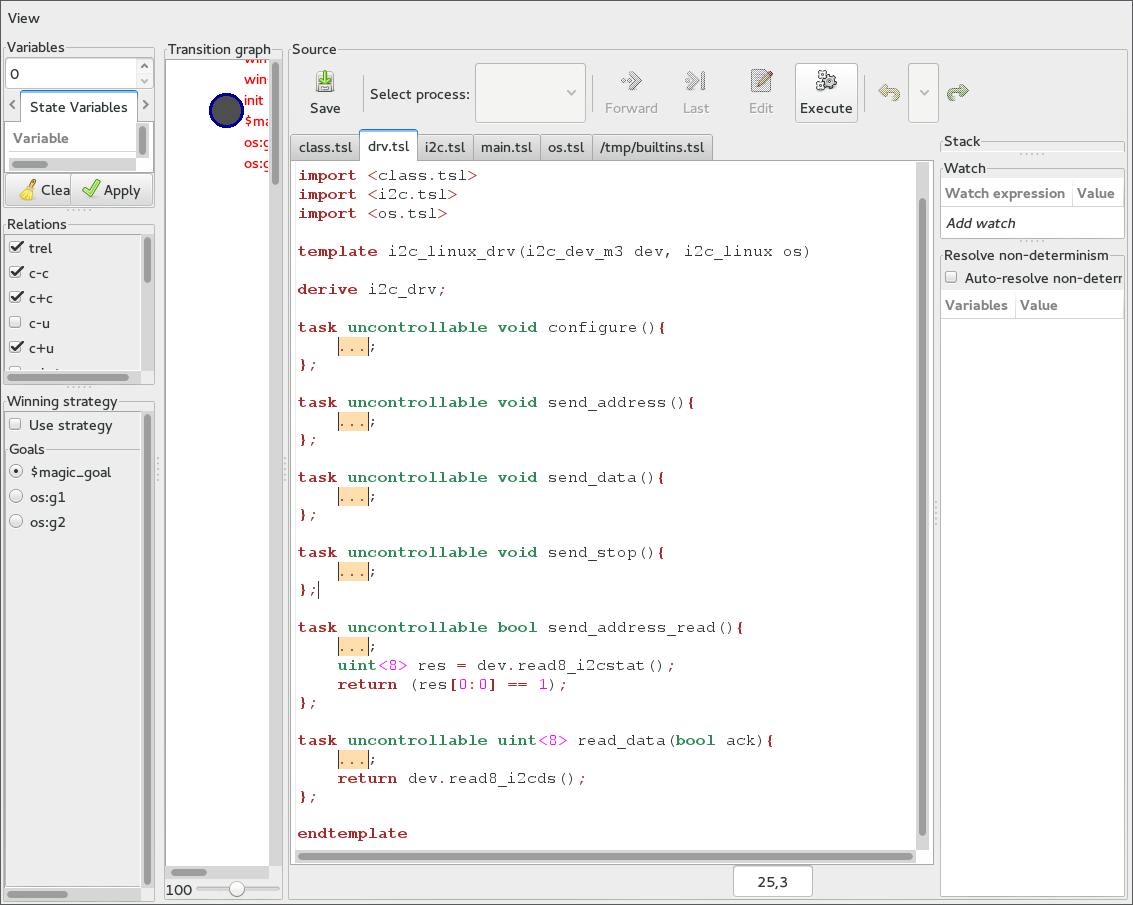
\includegraphics[width=\linewidth]{imgs/screenshot_1.png}
    \caption{Termite driver source code tab}
    \label{fig:driver_tab}
\end{figure}

\begin{figure}
    \center
    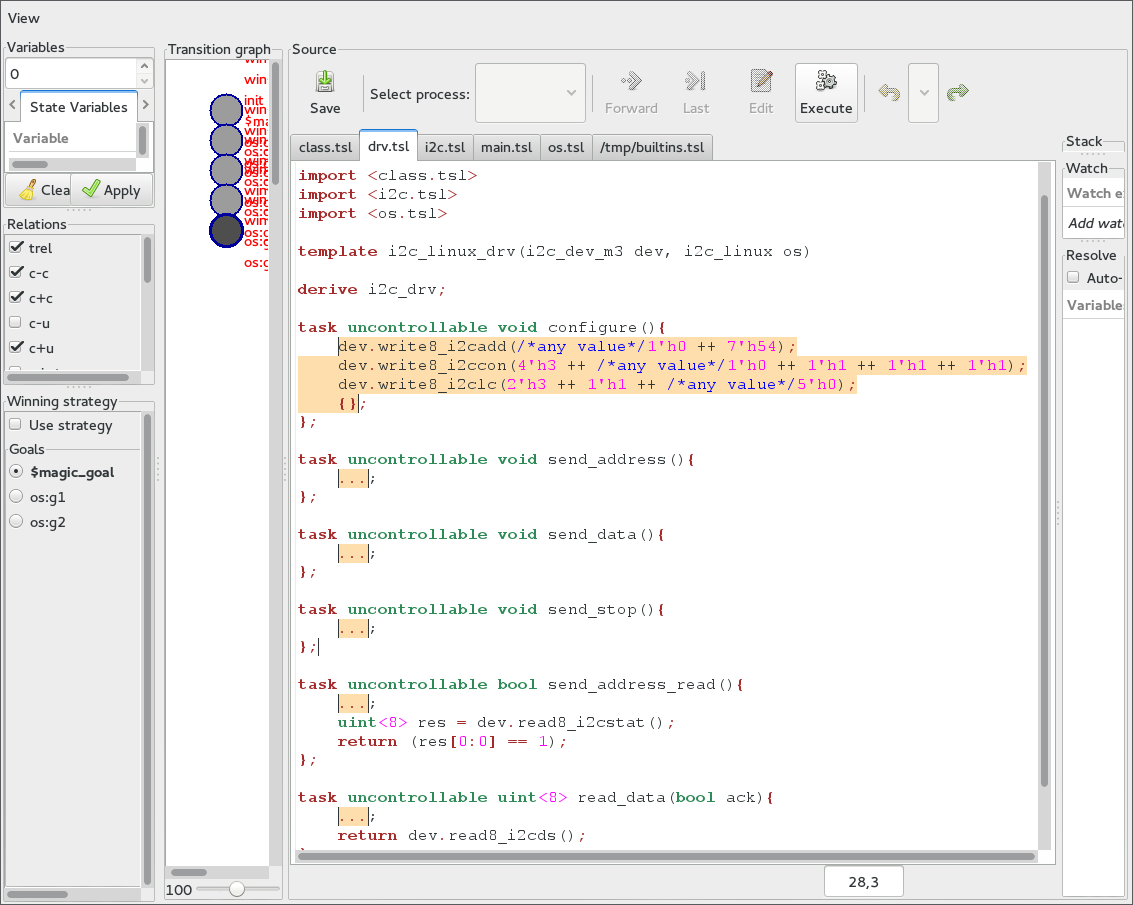
\includegraphics[width=\linewidth]{imgs/screenshot_2.png}
    \caption{Termite driver source code tab after code generation}
    \label{fig:driver_tab_gen}
\end{figure}

\section{Master write}
\label{a:sec_master_write}

\subsection{OS specification}
We continue from where we left off in the \code{pos} process in the OS specification. We first set a flag to signal that initialisation was successful and then we enter a forever loop (Section~\ref{sec:loops}). On each iteration, the loop non-deterministically chooses between performing a master read or a master write transaction. We do not cover synthesis of the master read transaction. Assuming execution of the process enters the \code{master\_write} function we end up at line~\ref{l:os_master_write}.

This function models the behavior we expect of the \code{send\_address}, \code{send\_data} and \code{send\_stop} sequence of driver functions. It uses a state variable \code{master\_state} to keep track of the current state of the master transmission. 

Note the two \emph{virtual callbacks} (similar to virtual functions) \code{address\_written} and \code{data\_sent} defined on lines~\ref{l:os_address_written} and~\ref{l:os_data_sent} respectively. They are invoked by the device state machine when the address writing and data sending phases complete. 

\subsection{Device specification}
As with configuration, the device specification must provide the mechanism for the driver to perform the master write transaction. Again this is performed through register writes such as \code{write8\_i2cstat} on line~\ref{l:dev_write8_i2cstat}. Observe that if bit 5 is set and there is currently no master transaction in progress, in addition to writing to the internal register, the write initiates a transaction by setting the enumeration \code{master\_transmit\_st} to \code{transmitting\_adddress\_t}. 

Process \code{pmaster} (line~\ref{l:dev_pmaster}) is the main device process responsible for performing the master transaction. \code{pmaster} is non-deterministically scheduled to run when events happen in the master state machine. When 
$$
\code{master\_transmit\_st} == \code{transmitting\_address\_t} 
$$
(as set by a previous write to \code{i2cstat}) on line~\ref{l:dev_pmaster_ta} it signals to the operating system that the address was written using the \code{address\_written} callback on line~\ref{l:dev_pmaster_aw}, which triggers the operating system to update its internal state.

Process \code{pmaster} handles data and stop bit transmission in the same way.

\subsection{Synthesizing}

\begin{figure}
    \center
    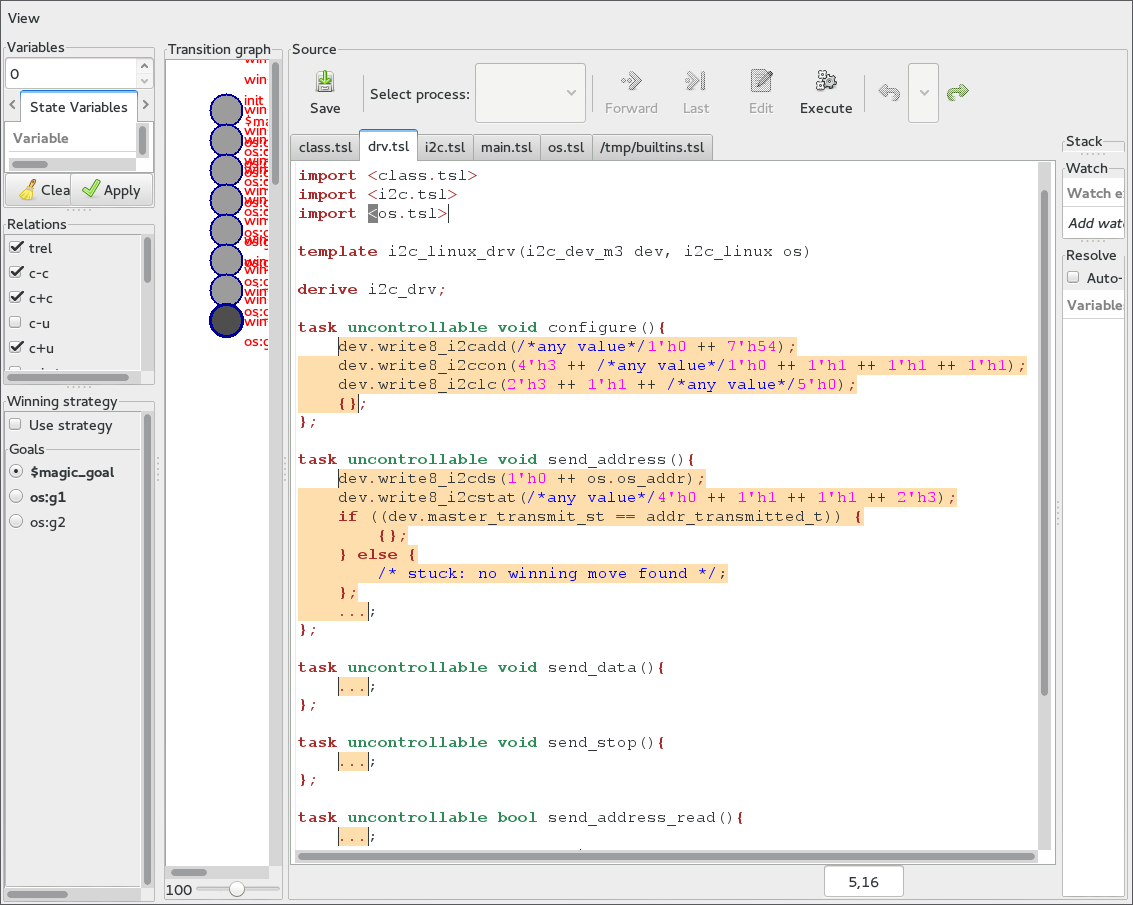
\includegraphics[width=\linewidth]{imgs/screenshot_3.png}
    \caption{Termite driver source code tab. Sending address.}
    \label{fig:driver_tab_addr}
\end{figure}

We proceed to generate code as we did for configuration. Code generation for \code{send\_address()} is shown in Figure~\ref{fig:driver_tab_addr}. The first two lines are generated automatically as before. However, on the third line, Termite gets stuck. It generates an if condition that says that if the device specification internal state variable \code{master\_transmit\_st} is equal to \code{addr\_transmitted\_t} then we can return from this function, otherwise, Termite is stuck. There are two problems with this code: the device internal variable is not accessible to the driver, and, one branch of the if statement is a dead end. 

This is actually Termite's rather cryptic way of saying that the correct action is to wait until $\code{dev.master\_transmit\_st} == \code{addr\_transmitted\_t}$. This corresponds to waiting until the address is transmitted, which is what you would expect. The driver developer can verify this by replacing the entire if condition with 

$$\code{wait(dev.master\_transmit\_st} == \code{addr\_transmitted\_t})$$.

This is a manifestation of the white box assumption that Termite makes. It assumes that the driver can access all of the system's state variables. To remedy this, manual intervention is needed. Consultation of the device manual tells us that after the address is sent the device sets bit 4 of \code{i2ccon} to one. So, we manually write code to loop while this bit is zero (line~\ref{l:drv_manual_loop}). We then re-run Termite with the amended driver and Termite checks that the manually written code is correct. Synthesis with the manually written code succeeds and, again, Termite creates the window shown in Figure~\ref{fig:driver_tab_addr_man}, verifying that the code is correct. So, while we were forced to write code manually, Termite was able to verify that is was correct.

\begin{figure}
    \center
    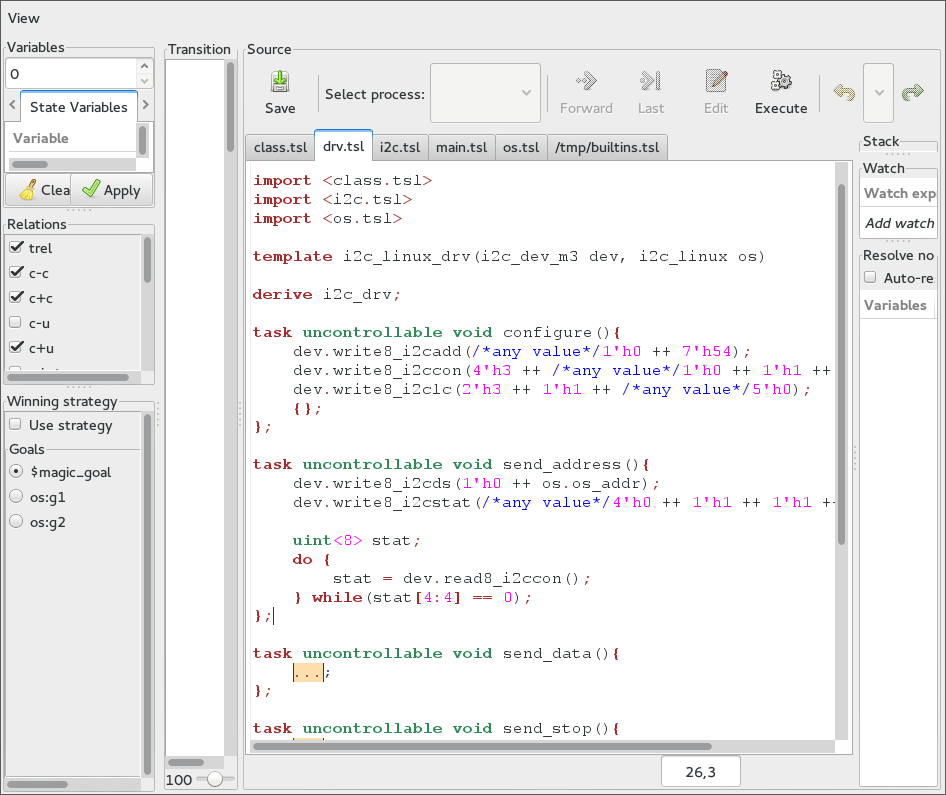
\includegraphics[width=\linewidth]{imgs/screenshot_4.png}
    \caption{Termite driver source code tab. Sending address manual code.}
    \label{fig:driver_tab_addr_man}
\end{figure}

We proceed in exactly the same way for the remaining functions \code{send\_data()} and \code{send\_stop()}. Each function requires us to manually work around the white box assumption as we did for \code{send\_address()}. The final driver is shown in Listing~\ref{lst:synth}.

\section{Specifications}

In this section we give all specifications in full. In addition to the specifications already discussed, we also give the class specification (Listing~\ref{lst:class_spec}) and the main file (Listing~\ref{lst:main}). The class specification is much like C header and it declares datatypes and the externally visible interface to the other specifications. The main file creates an instance of each specification and ties them together.

\vspace*{5mm}
\lstinputlisting[style=tsl2, caption=OS specification, label=lst:os_spec]{i2c/os.tsl}
\vspace*{5mm}
\lstinputlisting[style=tsl2, caption=Device specification, label=lst:dev_spec]{i2c/i2c.tsl}
\vspace*{5mm}
\lstinputlisting[style=tsl2, caption=Class specification, label=lst:class_spec]{i2c/class.tsl}
\vspace*{5mm}
\lstinputlisting[style=tsl2, caption=Main file, label=lst:main]{i2c/main.tsl}
\vspace*{5mm}
\lstinputlisting[style=tsl2, caption=Synthesized driver, label=lst:synth]{i2c/drv.tsl.synthesized}



\backmatter
\cleardoublepage
\bibliographystyle{thesisnat}
\bibliography{bibtex/fm.bib,bibtex/systems.bib,extra.bib}

\end{document}
